\documentclass[aspectratio=169]{beamer}

%---------------------------------------------------------------------
% UMN Custom Beamer Theme Preamble
%---------------------------------------------------------------------
% shared import of packages and command definitions for slides and text

\usepackage{silence} % silence warnings
% dont have tikz-feynman tell me LuaTex would be better on every vertex and line
\WarningFilter{tikz-feynman}{The key you tried}

\usepackage{epsfig} % Allows the inclusion of eps files
\usepackage{epic} % Enhanced picture mode
\usepackage{eepic} % Extensions for epic
\usepackage{url} % URL handling
\usepackage{longtable} % Tables that continue onto multiple pages
\usepackage{mathrsfs} % Support for \mathscr script
\usepackage{multirow} % Span rows in tables
\usepackage{bigstrut} % Space struts in tables up and down
\usepackage{amssymb} % AMS math symbols and helpers
\usepackage{graphicx} % Enhanced graphics support
\usepackage{setspace} % Adjust spacing in captions, single by default
\usepackage{xspace} % Automatically adjusting space after macros
\usepackage{amsmath} % \text, and other math formatting options
\usepackage[version=4]{mhchem} % For chemistry equations (e.g. Colbalt decay in Wu experiment)
\usepackage{siunitx} % \num{} formatting and SI unit formatting
\usepackage{booktabs} % Enhanced tables with \toprule, etc.
\usepackage{hyperref} % Add clickable links to other parts of the document
\usepackage{subcaption}
\usepackage{graphicx} % Allows including images
\usepackage{relsize} % for \smaller in \babar

\usepackage[noabbrev,capitalise]{cleveref} % Automatically determine \cref type

% Configure the cleveref package
\newcommand{\creflastconjunction}{, and } % Always use the serial comma

\usepackage[compat=1.1.0]{tikz-feynman} % for feynman diagrams
\tikzfeynmanset{
    warn luatex = {false}
}

\usepackage{hepunits}
% Configure the siunitx package
\sisetup{
    group-separator = {,}, % Use , to separate groups of digits, like 12,345
    list-final-separator = {, and } % Always use the serial comma in \SIlist
}

\newcommand{\fourgev}{\qty{4}{GeV}\xspace}
\newcommand{\eightgev}{\qty{8}{GeV}\xspace}
\newcommand{\ecal}{ECal\xspace}
\newcommand{\hcal}{HCal\xspace}

% absolute, official way according to Bertrand
\newcommand{\babar}{%
  \mbox{\slshape B\kern-0.1em{\smaller A}\kern-0.1em B\kern-0.1em{\smaller A\kern-0.2em R}}%
  \xspace
}

\usepackage{acronym}
\acrodef{dm}[DM]{Dark Matter}
\acrodef{sm}[SM]{Standard Model}
\acrodef{gr}[GR]{General Relativity}
\acrodef{cmb}[CMB]{Cosmic Microwave Background}
\acrodef{bao}[BAO]{Baryon Acoustic Oscillations}
\acrodef{hep}[HEP]{High Energy Physics}
\acrodef{wimp}[WIMP]{Weakly Interacting Massive Particle}
\acrodef{ecal}[ECal]{Electromagnetic Calorimeter}
\acrodef{hcal}[HCal]{Hadronic Calorimeter}
\acrodef{ldmx}[LDMX]{Light Dark Matter eXperiment}
\acrodef{hps}[HPS]{Heavy Photon Search experiment}
\acrodef{jlab}[JLab]{Thomas Jefferson National Accelerator Laboratory}
\acrodef{cebaf}[CEBAF]{Continuous Electron Beam Accelerator Facility}
\acrodef{kf}[KF]{Kalman Filter}
\acrodef{gbl}[GBL]{General Broken Lines}
\acrodef{svt}[SVT]{Silicon Vertex Tracker}
\acrodef{bdt}[BDT]{Boosted Decision Tree}
\acrodef{eot}[EoT]{Electrons on Target}
\acrodef{eat}[EaT]{\ac{ecal} as Target}
\acrodef{mm}[MM]{Missing Momentum}
\acrodef{simp}[SIMP]{Strongly-Interacting Massive Particle}
\acrodef{vps}[VPS]{Vertex Projection Significance}
\acrodef{fee}[FEE]{Full Energy Electron}
\acrodef{oim}[OIM]{Optimum Interval Method}
\acrodef{pe}[PE]{photoelectrons}

\def\minyzero{$y_{0,\min}$\xspace}
\def\maxyzeroerr{$\sigma_{y_0,\max}$\xspace}
\def\Psum{$P_\mathrm{sum}$\xspace}

%Environment for drawing on pictures using tikz
%   #1 Width to adjust image to (default: \textwidth)
%   #2 Filepath to image
%Use like:
%   \begin{tikzimage}[height]{filepath}
%       ...\draw...( coordinates are in fractions of width/height of image )
%   \end{tikzimage}
\newenvironment{tikzimage}[2][\textwidth]{%
    \begin{tikzpicture}
        \node[anchor=south west, inner sep=0] (image) at (0,0)
            {\includegraphics[width=#1]{{#2}}};
        \begin{scope}[x={(image.south east)},y={(image.north west)}]
}{%
        \end{scope}
    \end{tikzpicture}
}%


% HPS Diagrams
%   using tikz math library to name variables to helpful names
%   define command to draw boilerplate target/L1/L2
\usetikzlibrary{math,decorations.pathreplacing}
   
% colors for diagram
\definecolor{HPSTarget}{rgb}{0.55,0.52,0.54}
\definecolor{HPSTracker}{rgb}{0.0,0.5,0.5}
\definecolor{HPSEcal}{rgb}{0.8,0.5,0.2}

\tikzmath{%
  \openingslope = 0.15; % y changer per x change
  \sensorsep = 0.12; % separation between sensors in a layer
  \sensorlen = 1.5; % length of sensors in vertical direction
  \targetx = -3.0;
  \layeronex = -0.2;
  \layertwox = 2.0;
  \targethalfthick = 0.1;
  \ecalbarlen=1.5;
  \ecalbarwidth=0.3;
  % can't have a blank line in this block
  %
  % compute locations
  \layeroney = (\layeronex - \targetx) * \openingslope;
  \layertwoy = (\layertwox - \targetx) * \openingslope;
  \sensorhalfsep = \sensorsep / 2;
  \reflineendx = \layertwox+0.5;
  \reflineendy = (\reflineendx - \targetx) * \openingslope;
  % paths for truly displaced
  \eleslope=(2-0.1)/(2.5-\targetx-2);
  \eleyzero=\eleslope*(-2.0)+0.1;
  \elelayeronestereoy=\eleslope*(\layeronex - \sensorhalfsep+1.0)+0.1;
  \elelayeroneaxialy=\eleslope*(\layeronex + \sensorhalfsep+1.0)+0.1;
  \elelayertwostereoy=\eleslope*(\layertwox - \sensorhalfsep+1.0)+0.1;
  \elelayertwoaxialy=\eleslope*(\layertwox + \sensorhalfsep+1.0)+0.1;
  \posslope=(-1.8-0.1)/(2.5-\targetx-2);
  \posyzero=\posslope*(-2.0)+0.1;
  \poslayeronestereoy=\posslope*(\layeronex - \sensorhalfsep+1.0)+0.1;
  \poslayeroneaxialy=\posslope*(\layeronex + \sensorhalfsep+1.0)+0.1;
  \poslayertwostereoy=\posslope*(\layertwox - \sensorhalfsep+1.0)+0.1;
  \poslayertwoaxialy=\posslope*(\layertwox + \sensorhalfsep+1.0)+0.1;
  % paths for not displaced
  \ndeleslope = (2-0)/(2.5-\targetx-\targethalfthick);
  \ndelelayeronestereoy=\ndeleslope*(\layeronex - \sensorhalfsep - \targetx - \targethalfthick);
  \ndelelayeroneaxialy=\ndeleslope*(\layeronex + \sensorhalfsep - \targetx - \targethalfthick);
  \ndelelayertwostereoy=\ndeleslope*(\layertwox - \sensorhalfsep - \targetx - \targethalfthick);
  \ndelelayertwoaxialy=\ndeleslope*(\layertwox + \sensorhalfsep - \targetx - \targethalfthick);
  \ndposslope = (-1.8-0)/(2.5-\targetx-\targethalfthick);
  \ndposlayeronestereoy=\ndposslope*(\layeronex - \sensorhalfsep - \targetx - \targethalfthick);
  \ndposlayeroneaxialy=\ndposslope*(\layeronex + \sensorhalfsep - \targetx - \targethalfthick);
  \ndposlayertwostereoy=\ndposslope*(\layertwox - \sensorhalfsep - \targetx - \targethalfthick);
  \ndposlayertwoaxialy=\ndposslope*(\layertwox + \sensorhalfsep - \targetx - \targethalfthick);
  % paths for fake displaced
  \fdeleslope = (2-0)/(2.5-\targetx-\targethalfthick);
  \fdelelayeronestereoy=\fdeleslope*(\layeronex - \sensorhalfsep - \targetx - \targethalfthick);
  \fdelelayeroneaxialy=\fdeleslope*(\layeronex + \sensorhalfsep - \targetx - \targethalfthick);
  \fdelelayertwostereoy=\fdeleslope*(\layertwox - \sensorhalfsep - \targetx - \targethalfthick);
  \fdelelayertwoaxialy=\fdeleslope*(\layertwox + \sensorhalfsep - \targetx - \targethalfthick);
  \fdposx = \targetx+1.0;
  \fdposy = \fdeleslope*(\fdposx-\targetx-\targethalfthick);
  \fdposslope = (-1.8-\fdposy)/(2.5-\fdposx);
  \fdposyzero = \fdposslope*(\targetx-\fdposx)+\fdposy;
  \fdbadhitstereoy = \fdposslope*(\layeronex-\sensorhalfsep-\fdposx)+\fdposy;
  \fdbadhitaxialy = \fdposslope*(\layeronex+\sensorhalfsep-\fdposx)+\fdposy;
  \fdposlayertwostereoy=\fdposslope*(\layertwox - \sensorhalfsep - \fdposx)+\fdposy;
  \fdposlayertwoaxialy=\fdposslope*(\layertwox + \sensorhalfsep - \fdposx)+\fdposy;
  % true path is from center of target to L2 hits
  \fdpostruslope = (\fdposslope*(\layertwox-\fdposx)+\fdposy-0)/(\layertwox-\targetx-\targethalfthick);
  \fdtruhitstereoy = \fdpostruslope*(\layeronex-\sensorhalfsep-\targetx-\targethalfthick);
  \fdtruhitaxialy = \fdpostruslope*(\layeronex+\sensorhalfsep-\targetx-\targethalfthick);
}

\tikzset{
  vertex/.style={diamond,fill,inner sep=1.5pt},
  hit/.style={circle,fill,inner sep=1.5pt},
  miss/.style={circle,draw,fill=white,inner sep=1.0pt}
}

\newcommand{\drawhpsfirsttwolayers}{%
  \draw[HPSTracker, very thick]
    (\layeronex-\sensorhalfsep,-\layeroney-\sensorlen)
    -- (\layeronex-\sensorhalfsep,-\layeroney)
    (\layeronex+\sensorhalfsep,-\layeroney-\sensorlen)
    -- (\layeronex+\sensorhalfsep,-\layeroney)
    (\layeronex-\sensorhalfsep,\layeroney+\sensorlen)
    -- (\layeronex-\sensorhalfsep,\layeroney)
    (\layeronex+\sensorhalfsep,\layeroney+\sensorlen)
    -- (\layeronex+\sensorhalfsep,\layeroney);
  \draw[HPSTracker] (\layeronex,\layeroney+\sensorlen) node[above] {L1};
  
  \draw[HPSTracker, very thick]
    (\layertwox-\sensorhalfsep,-\layertwoy-\sensorlen)
    -- (\layertwox-\sensorhalfsep,-\layertwoy)
    (\layertwox+\sensorhalfsep,-\layertwoy-\sensorlen)
    -- (\layertwox+\sensorhalfsep,-\layertwoy)
    (\layertwox-\sensorhalfsep,\layertwoy+\sensorlen)
    -- (\layertwox-\sensorhalfsep,\layertwoy)
    (\layertwox+\sensorhalfsep,\layertwoy+\sensorlen)
    -- (\layertwox+\sensorhalfsep,\layertwoy);
  \draw[HPSTracker] (\layertwox,\layertwoy+\sensorlen) node[above] {L2};
  
  \draw[gray,dashed] (\targetx,0) -- (\reflineendx,\reflineendy);
  \draw[gray,dashed] (\targetx,0) -- (\reflineendx,0);
  \draw[gray,dashed] (\targetx,0) -- (\reflineendx,-\reflineendy);
  
  \fill[HPSTarget] (\targetx-\targethalfthick,+1) rectangle (\targetx+\targethalfthick,-1);
  \draw[HPSTarget] (\targetx,-1) node[below] {Target};
}

\newcommand{\drawhps}{%
  \foreach \layerX/\layerY in {
    0.0/0.15,
    2.0/0.30,
    4.0/0.45,
    6.0/0.60,
    8.0/0.75,
    10.0/0.90
  }{
    \draw[HPSTracker, very thick]
      (\layerX-\sensorhalfsep,-\layerY-\sensorlen)
      -- (\layerX-\sensorhalfsep,-\layerY)
      (\layerX+\sensorhalfsep,-\layerY-\sensorlen)
      -- (\layerX+\sensorhalfsep,-\layerY)
      (\layerX-\sensorhalfsep,\layerY+\sensorlen)
      -- (\layerX-\sensorhalfsep,\layerY)
      (\layerX+\sensorhalfsep,\layerY+\sensorlen)
      -- (\layerX+\sensorhalfsep,\layerY);
  }
  \draw[HPSTracker] (9.0,0.75+\sensorlen) node[above,font=\LARGE] {SVT};

  \foreach \barY in {
    0.9,
    1.2,
    1.5,
    1.8,
    2.1
  }{
    \draw[draw=HPSEcal,fill=HPSEcal!20!white]
      (12.0,\barY) rectangle (12+\ecalbarlen,\barY+\ecalbarwidth)
      (12.0,-\barY) rectangle (12+\ecalbarlen,-\barY-\ecalbarwidth)
    ;
  }
  \draw[HPSEcal] (12+\ecalbarlen/2,2.1+\ecalbarwidth) node[above,font=\LARGE] {ECal};

  \draw[gray,dashed] (\targetx,0) -- (12+\ecalbarlen+0.5,0);
  
  \fill[HPSTarget] (\targetx-\targethalfthick,+1) rectangle (\targetx+\targethalfthick,-1);
  \draw[HPSTarget] (\targetx,-1) node[below left,font=\LARGE] {Target};

  \node (decay) at (\targetx+1.0,0.05) [circle,fill,inner sep=1.5pt] {};
  \node (production) at (\targetx,0.0) [circle,fill,inner sep=1.5pt] {};

  \draw[black,very thick,->]
    (\targetx-1.5,0.0) node[anchor=south east,font=\Large] {\(e^-\)} -- (\targetx-0.2,0.0);
  \draw[black,very thick,->]
    (decay) -- (11.8,1.6) node[anchor=south east,font=\Large] {\(e^-\)};
  \draw[black,very thick,->]
    (decay) -- (11.8,-2.2) node[anchor=north east,font=\Large] {\(e^+\)};
  \draw[black,very thick,->]
    (production) -- (-1.0,-0.5-\sensorlen) node[anchor=east,font=\Large] {\(e^-\)};

  \draw[blue,thick,->] (production) -- (decay) node[midway,above,font=\Large] {\(V_D\)};
}
 % External preamble for general packages
% Note: Ensure that TikZ, xspace and other dependencies are loaded here if not loaded below

%---------------------------------------------------------------------
% Geometry Adjustments
%---------------------------------------------------------------------
\geometry{mag=1600,truedimen} % Adjust layout scaling

%---------------------------------------------------------------------
% UMN Color Definitions (University of Minnesota colors)
%---------------------------------------------------------------------
\definecolor{UMNMaroon}{RGB}{122,0,25}
\definecolor{UMNLightGold}{RGB}{255,215,95}
\definecolor{UMNGold}{RGB}{255,204,51}
\definecolor{UMNStormy}{RGB}{64,77,91}
\definecolor{UMNSunny}{RGB}{0,149,182}
\definecolor{UMNLightGray}{RGB}{213,214,210}

\definecolor{GopherMaroon}{RGB}{122, 0, 25}
\definecolor{GopherGold}{RGB}{255, 204, 51}
\definecolor{GopherLightGold}{RGB}{255, 222, 122}
\definecolor{GopherDarkMaroon}{RGB}{91, 0, 19}

%---------------------------------------------------------------------
% Packages specific to this theme
%---------------------------------------------------------------------
\usepackage{textpos}    % For precise positioning
\usepackage{epstopdf}    % Convert EPS images to PDF
\usepackage{soul}        % For highlighting and letter spacing
\usepackage{xifthen}     % For conditional logic in commands
\usepackage{listings}    % For code listings

% Define a custom background color for listings if needed
%\definecolor{backcolour}{rgb}{0.95,0.95,0.92} % Consider using this for consistency

%---------------------------------------------------------------------
% Listing Style Definition
%---------------------------------------------------------------------
\lstdefinestyle{mystyle}{
    backgroundcolor=\color{UMNLightGray},
    commentstyle=\color{UMNStormy},
    keywordstyle=\color{UMNMaroon},
    numberstyle=\tiny\color{UMNMaroon},
    stringstyle=\color{UMNSunny},
    basicstyle=\ttfamily\footnotesize,
    emph={ldmx}, % Note: Ensure no trailing spaces unless intentional
    emphstyle=\color{UMNMaroon},
    breakatwhitespace=false,
    breaklines=true,
    captionpos=b,
    keepspaces=true,
    numbers=left,
    numbersep=5pt,
    showspaces=false,
    showstringspaces=false,
    showtabs=false,
    tabsize=2
}
\lstset{style=mystyle}

%---------------------------------------------------------------------
% Custom Commands and Environments
%---------------------------------------------------------------------

% Bold and color text command.
\newcommand{\boldcol}[2]{%
    {\color{#1}\textbf{#2}}\xspace
}%

% Slide section title command for intra-slide division.
\newcommand{\framesection}[1]{%
  \boldcol{UMNStormy}{#1}\hspace{1em}%
}%

% Code inclusion commands for listings.
\newcommand{\codefile}[2]{%
    \lstinputlisting[#1]{#2}
}%

\newcommand{\code}[1]{%
  \tikz[baseline=(codebox.base)]{
    \node[inner sep=1pt,outer sep=0pt,draw=UMNStormy,line width=0.05mm,fill=UMNLightGray,rounded corners=0.03cm] (codebox) 
      {\textcolor{UMNSunny}{#1}};
  }%
}%

% Checkmark and crossmark definitions using bbding.
\usepackage{bbding}
\newcommand{\checkmarkicon}{{\color{UMNSunny}\Checkmark}}
\newcommand{\crossmarkicon}{{\color{UMNMaroon}\XSolidBrush}}

% List item markers for done, todo, good, and bad items.
\newcommand{\done}{\item[$\color{UMNMaroon}\boxtimes$]}
\newcommand{\todo}{\item[$\color{UMNMaroon}\square$]}
\newcommand{\good}{\item[\checkmarkicon]}
\newcommand{\bad}{\item[\crossmarkicon]}

% Hyperlink button command
\newcommand{\hlink}[2]{%
    \href{#1}{\beamergotobutton{#2}}
}%

% Slide layout commands for including plots/images.
\newcommand{\oneplotslide}[3]{% #1=Title, #2=Subtitle, #3=Image path
    \begin{frame}
        \frametitle{#1}
        \framesubtitle{#2}
        \begin{figure}
            \centering
            \includegraphics[width=\textwidth,height=0.8\textheight,keepaspectratio]{#3}
        \end{figure}
    \end{frame}
}%

\newcommand{\fourtileslide}[6]{% #1=Title, #2=Subtitle, #3-#6=Tile contents
    \begin{frame}
        \frametitle{#1}
        \framesubtitle{#2}
        \begin{figure}[h]
            \centering
            \begin{tabular}{cc}
                #3 & #4 \\
                #5 & #6
            \end{tabular}
        \end{figure}
    \end{frame}
}%

\newcommand{\fourplotslide}[6]{%
    \fourtileslide{#1}{#2}%
        {\ifthenelse{\isempty{#3}}{}{ \includegraphics[height=0.4\textheight]{#3}}}%
        {\ifthenelse{\isempty{#4}}{}{ \includegraphics[height=0.4\textheight]{#4}}}%
        {\ifthenelse{\isempty{#5}}{}{ \includegraphics[height=0.4\textheight]{#5}}}%
        {\ifthenelse{\isempty{#6}}{}{ \includegraphics[height=0.4\textheight]{#6}}}%
}%

% Environment for a slide with a picture and accompanying comments.
\newenvironment{figurecomments}[1]{% #1=Image path
  \begin{columns}
    \begin{column}{0.6\textwidth}
      \begin{figure}
        \centering
        \includegraphics[height=0.7\textheight]{#1}
      \end{figure}
    \end{column}
    \begin{column}{0.4\textwidth}
      \footnotesize
}{%
    \end{column}
  \end{columns}
}%

% A full slide for section titles.
\newcommand{\sectionframe}[1]{%
  \begin{frame}
    \vfill
    \centering
    \begin{beamercolorbox}[sep=8pt,center,shadow=true,rounded=true]{title}
        \usebeamerfont{title}#1\par%
    \end{beamercolorbox}
    \vfill
  \end{frame}
}%

% Backup slides environment to exclude from main slide count.
\newenvironment{backup}[1][Questions]{%
  \sectionframe{#1}%
  \newcounter{finalframe}%
  \setcounter{finalframe}{\value{framenumber}}%
}{%
  \setcounter{framenumber}{\value{finalframe}}%
}%

%---------------------------------------------------------------------
% Beamer Presentation Mode Settings
%---------------------------------------------------------------------
\mode<presentation> {
  \usetheme{Madrid}
  \usefonttheme{serif}
  % Add logos to slide header (customize positioning as needed)
  \addtobeamertemplate{frametitle}{}{%
      \begin{textblock*}{100mm}(0.8\textwidth,-0.95cm)
          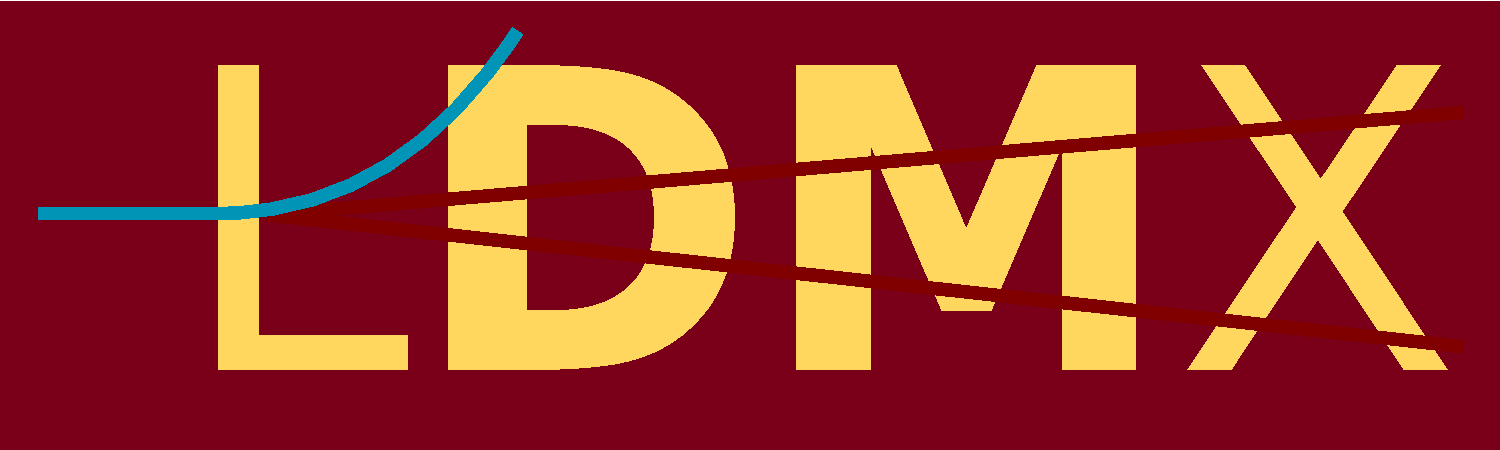
\includegraphics[height=0.95cm]{ldmx_logo}
      \end{textblock*}
      \begin{textblock*}{100mm}(0.7\textwidth,-0.95cm)
          
\includegraphics[height=0.95cm]{heavy_photon_logo}
      \end{textblock*}
  }

  % Beamer color definitions and palette
  %\setbeamercolor{structure}{fg=UMNStormy}
  \setbeamercolor{structure}{fg=UMNStormy} % Colors blocks and the 'Figure' caption heading. Default fg=UMNStormy.
  \setbeamercolor{palette primary}{fg=UMNMaroon, bg=UMNLightGray} % Default fg=UMNMaroon, bg=UMNLightGray.
  \setbeamercolor{palette secondary}{fg=UMNMaroon, bg=white}
  \setbeamercolor{palette tertiary}{fg=UMNLightGold, bg=UMNStormy}
  \setbeamercolor{frametitle}{fg=UMNLightGold, bg=UMNMaroon}
  \setbeamercolor{title}{fg=UMNMaroon, bg=UMNLightGray}
  \setbeamercolor{section in toc}{fg=UMNMaroon}
  \setbeamercolor{section in toc shaded}{fg=UMNMaroon}
  \setbeamercolor{button}{fg=UMNLightGold, bg=UMNMaroon}
  \setbeamercolor{palette sidebar secondary}{fg=UMNMaroon}
  \setbeamercolor{section in sidebar shaded}{fg=UMNMaroon}

  \setbeamertemplate{itemize item}{\color{UMNMaroon}$\blacksquare$}
  \setbeamertemplate{itemize subitem}{\color{UMNLightGold}$\blacktriangleright$}
  \setbeamertemplate{enumerate items}[default]
  \setbeamertemplate{sections/subsections in toc}[sections numbered]

  % Remove navigation symbols if not needed
  \setbeamertemplate{navigation symbols}{}

  \setbeamercolor{block body alerted}{fg=UMNSunny, bg=UMNMaroon!20}
  \setbeamercolor{block title alerted}{fg=UMNLightGold, bg=UMNMaroon}
}

%---------------------------------------------------------------------
% Author and Institution Details
%---------------------------------------------------------------------
\newcommand{\with}{} % Placeholder; fill or remove if not needed

\author{Billy Jackson} % Your name
\institute[UMN]{%
%  he/him/his \\[2mm]
  University of Minnesotas \\[2mm]
  \href{mailto:jack1851@umn.edu}{jack1851@umn.edu} \\[2mm]
  \begin{tabular}{p{0.4\textwidth}}\centering\with\end{tabular}
}

\usepackage{pgfpages}
\setbeamertemplate{note page}[plain]
\setbeameroption{show notes}
\addtobeamertemplate{note page}{}{\thispdfpagelabel{notes:\insertframenumber}}

\newcommand{\ssection}[1]{%
  \section{#1}%
  \sectionframe{#1}%
}%

\newenvironment{sframe}[1]{%
  \subsection{#1}%
  \begin{frame}{#1}%
}{%
  \end{frame}%
}%

\title[$\mathrm{W_R}$ Boson and Heavy Neutrino Search]{%
  Search for a Right-Handed W Boson and Heavy Neutrino of the Left-Right Symmetric Standard Model%
}

\begin{document}

\begin{frame}
  \maketitle
\end{frame}

\note[itemize]{
\item Hello everyone! For those of you who don't know me, my name is Billy.
  I am one of Jeremy's graduate students here with the CMS group, and in this 
  seminar I am going to talk about our search for a right-handed W boson and 
  heavy neutrino of the Left-Right Symmetric Standard Model. 
}

%\begin{frame}{Outline}
%  \begin{columns}
%    \begin{column}{0.5\textwidth}
%      \tableofcontents
%    \end{column}
%    \begin{column}{0.5\textwidth}
%      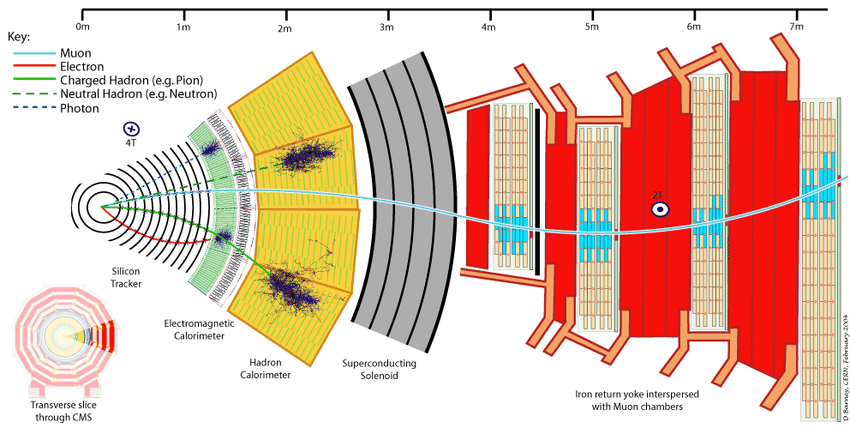
\includegraphics[width=0.9\textwidth]{../figures/experiment/cms-slice}
%      \\
%      \resizebox{0.9\textwidth}{!}{\begin{tikzpicture}
    \begin{feynman}
      %
      % -- Define the incoming quarks on the left
      \vertex (qbar) at (-2, 1.5) {\(\bar{q}'\)};
      \vertex (q)    at (-2,-1.5) {\(q\)};
      
      % -- Central vertex where q qbar' -> W_R
      \vertex [dot] (wr) at (0,0) {};
      
      % -- First decay: W_R -> N_\ell + l
      \vertex [dot] (Nl) at (2.5,0) {};
      \vertex (l1)  at (4,-1.5) {\(\ell^{+}\)};
      \vertex (N) at (4, 1.5) {};
      
      % -- Second decay: N_\ell -> l + W_R
      %    Then W_R -> 2 jets
      \vertex [dot] (wrl) at (4, 1.5) {};
      \vertex (l2) at (5.5,  3) {\(\ell^{-}\)};
      \vertex (wr2) at (6,  1) {};

      %    Then W_R -> 2 jets
      \vertex [dot] (jj) at (6, 1) {};
      \vertex (jet1) at (7.5,  1.7) {jet};
      \vertex (jet2) at (7.5, 0.3) {jet};
      
      % -- Draw the diagram
      \diagram*{
        % Incoming quarks
        (qbar) -- [fermion] (wr) -- [fermion] (q),
        
        % First decay of W_R
        (wr) -- [boson, edge label=\(W_R\)] (Nl),
        (l1) -- [fermion] (Nl),
        (Nl) -- [fermion, edge label=\(N_\ell\)] (wrl),
        
        % Decay of heavy neutrino N_l
        (wrl) -- [fermion] (l2),
        (wrl) -- [boson, edge label=\(W_R^{*}\)] (wr2),

        % Decay of second W_R into jets
        (jet1) -- [fermion] (jj) -- [fermion] (jet2),
      };
    \end{feynman}
  \end{tikzpicture}}
%    \end{column}
%  \end{columns}
%\end{frame}

%\note[itemize]{
%\item I will begin with some background, and explain the concept of handedness in physics.
%  So, what do we exactly mean when we say the weak force is left-handed and we are searching
%  for a right-handed W and neutrino.
%\item I will then discuss the class of models, called left-right symmetric models, 
%    that adds these particles to the standard model.
%\item We search for these particles using data from the CMS detector at the Large 
%  Hadron Collider, most people here familiar with these to some degree but I'll quickly
%  describe them.
%\item I will explain the general search strategy that we use to look for these particles 
%  using CMS data. 
%\item And then I will discuss our main backgrounds and how we are estimating them.
%\item Lastly, I'll end with a discussion about some of the things that we are looking
%  forward to in Run 3.
%}

\section{Background}

\subsection{Handedness and Weak Interactions}

\begin{frame}{Parity Violation in $\beta$ Decay}
  \begin{itemize}
    \item The parity operator $\hat{P}$ corresponds to a discrete 
      transformation $x \rightarrow -x$, etc.
    \item In 1957 C.S. Wu studied the beta decay:
      $\ce{^{60}_{27}Co \rightarrow ^{60}_{28}Ni + e^{-} + \bar{\nu_{e}}}$
  \end{itemize}
  \begin{columns}
    \begin{column}{0.65\textwidth}
      \begin{figure}
        \centering
        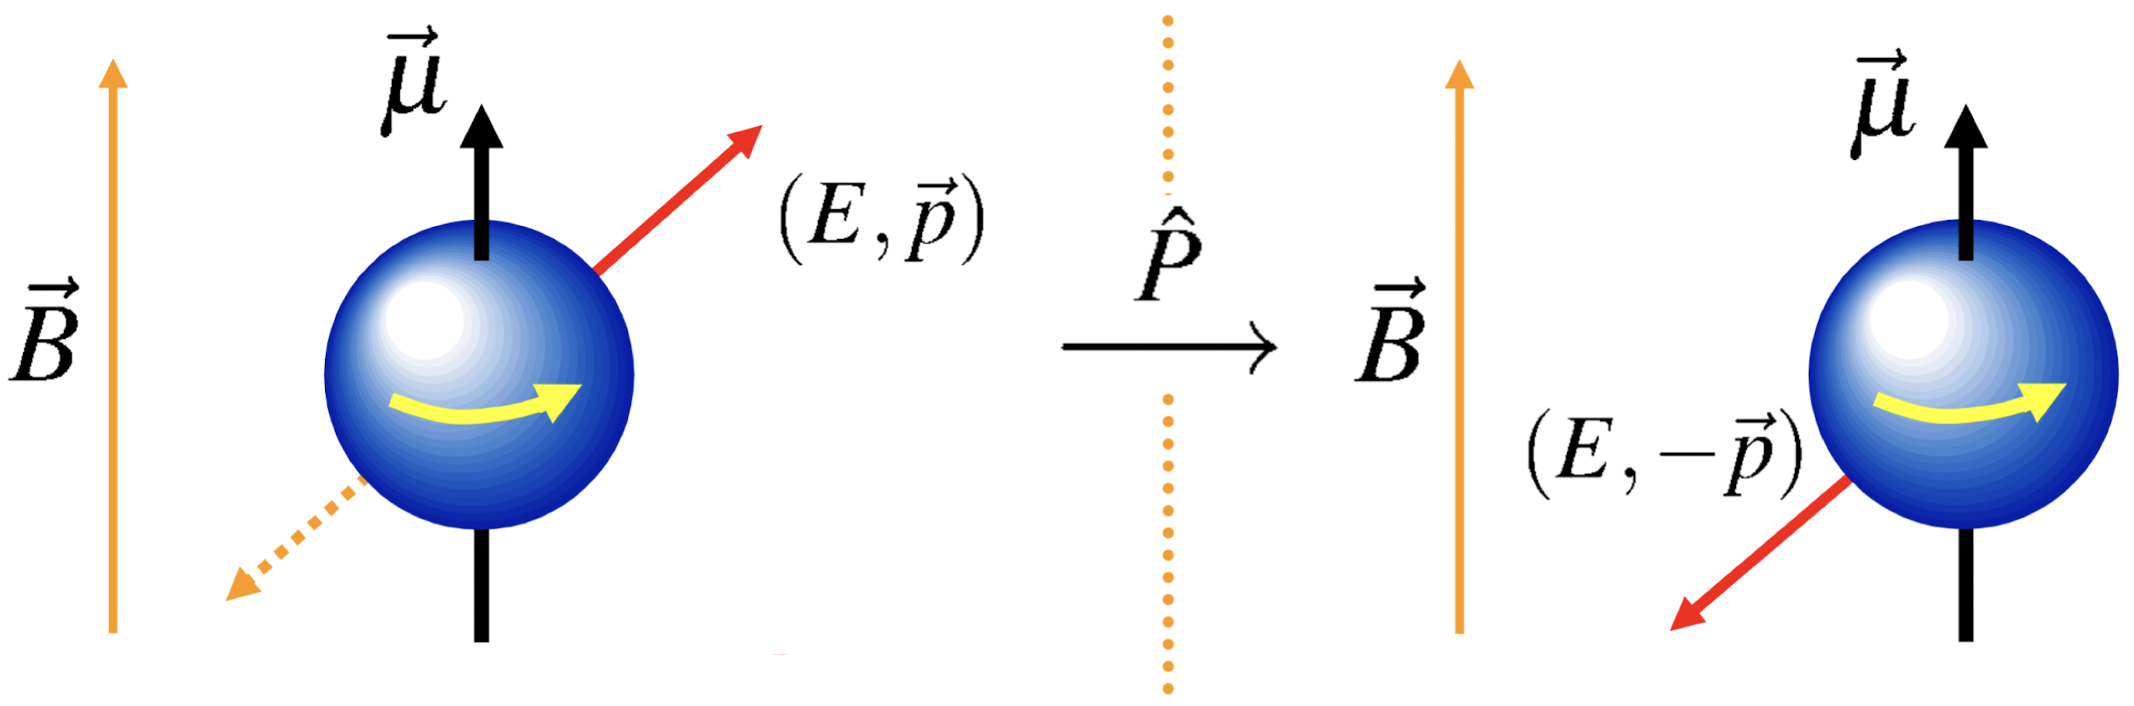
\includegraphics[width=\textwidth]{wu-experiment.png}
      \end{figure}
    \end{column}
    \begin{column}{0.3\textwidth}
      \begin{block}{}
        If parity were conserved: expect equal rate for producing $e^{-}$ in directions
            along and opposite to the nuclear spin.
      \end{block}
    \end{column}
  \end{columns}
  \begin{itemize}
    \item Observed \boldcol{UMNMaroon}{electrons emitted preferentially} in direction 
      opposite to applied field.
  \end{itemize}
  \begin{block}{}
    \centering
      Conclude \boldcol{UMNSunny}{parity is violated} in weak interactions.
  \end{block}
\end{frame}

\note[itemize]{
\footnotesize
\item No time for an outline, lets just dive right in. 
 The story really begins with the discovery of parity violation.
\item Parity symmetry (which is also informally some called the mirror symmetry) is the idea that for a given physical process, that
  process with its spatial coordinates inverted - or reflected in a mirror - 
  also represents another perfectly possible physical process.
\item And in 1957, Wu conducted this experiment in which she aligned the spins 
  of Cobalt-60 nuclei in a strong magnetic field. Cobalt-60 beta decays in a weak 
  interaction to nickel, an electron and antineutrino, and Wu recorded the directions 
  of the emitted electrons relative to the magnetic field. 
\item If we consider this process under a parity transformation, the only kinematic quantity that changes sign
  is the vector momentum of the emitted electrons, since the magnetic field and magnetic moment are
  both axial vectors. So, if parity were conserved in weak interactions, the rate at which electrons were
  emitted at a certain direction relative to the magnetic field would be identical to the rate in the opposite
  direction. And this is what they expected to find.
\item Experimentally however, it was observed that most electrons were emitted in the hemisphere opposite
  to the direction of the applied magnetic field, thus providing a clear demonstration that parity is violated 
  in weak interactions.
\item It was a bizarre and surprising result, with the implication being that the weak force is left-handed.
}

\begin{frame}{Helicity States}
  \begin{block}{Definition}
    Define the \boldcol{UMNSunny}{Helicity} of a particle as the projection of its spin onto the direction of momentum.
  \end{block}
  \begin{columns}
    \begin{column}{0.60\textwidth}
      \begin{figure}
        \centering
        % MU DECAY - maximal positron energy
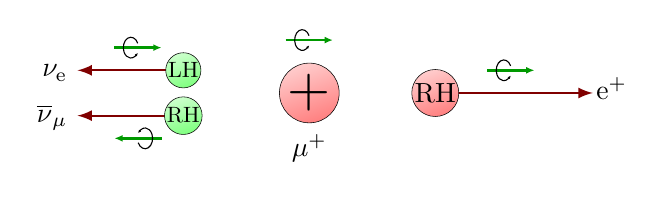
\begin{tikzpicture}[scale=2]
    % Local styling definitions
    \tikzset{>=latex} % set arrow head style
  
    % Color definitions
    \colorlet{vcol}{red!50!black}
    \colorlet{Scol}{green!60!black}
    
    % TikZ style definitions
    \tikzstyle{velocity}  =[->,thick,vcol]
    \tikzstyle{spin}      =[->,very thick,Scol]
    \tikzstyle{charge+}   =[very thin,draw=black,
                             top color=red!20!white, bottom color=red!50!white,
                             shading angle=20,circle,inner sep=0.2]
    \tikzstyle{charge0}   =[very thin,draw=black,
                             top color=green!20!white, bottom color=green!50!white,
                             shading angle=20,circle,inner sep=0.2]
  
    % Custom pic: spin (with a local length variable)
    \tikzset{
      pics/spin/.style={
        code={
          \def\Lspin{0.6} % Increased from 0.38 to 0.6 for longer spin arrows
          \draw[-{Latex[length=3,width=2.5]},pic actions,rotate=#1,line width=0.9,Scol]
            (-\Lspin/2,0) -- ++(\Lspin,0);
          \draw[pic actions,rotate=#1,thin,white]
            (-0.15*\Lspin,0) ++(170:{0.16*\Lspin} and {0.22*\Lspin}) arc (170:190:{0.16*\Lspin} and {0.22*\Lspin});
          \draw[-{Latex[length=1.2,width=1]},pic actions,rotate=#1,thin]
            (-0.15*\Lspin,0) ++(25:{0.16*\Lspin} and {0.22*\Lspin}) arc (25:305:{0.16*\Lspin} and {0.22*\Lspin})
            -- ++(50:0.09*\Lspin);
        }
      },
      pics/spin/.default=90,
    }
  
    % Drawing definitions
    \def\L{0.8}
    \def\v{1.2*\L}
    \coordinate (O) at (0,0);
    \coordinate (LT) at (-\L, 0.18*\L);
    \coordinate (LB) at (-\L,-0.18*\L);
    \coordinate (R) at (\L,0);
    \coordinate (T) at (0,0.42*\L);
    \coordinate (LTS) at ($(LT)+(-0.3*\v, 0.18*\L)$);
    \coordinate (LBS) at ($(LB)+(-0.3*\v,-0.18*\L)$);
    \coordinate (RS) at ($(R)+(0.50*\v,0.18*\L)$);
    
    % Vectors
    \draw[->,velocity] (R)++(0.05*\L,0) -- ++(\v,0);
    \draw[->,velocity] (LT) --++ (-0.7*\v,0) node[black,above=2,left=0] {\strut$\nu_\mathrm{e}$};
    \draw[->,velocity] (LB) --++ (-0.7*\v,0) node[black,below=3,left=0] {\strut$\overline{\nu}_\mu$};
    
    % Spin pictograms
    \pic at (RS)  {spin={  0}};
    \pic at (LTS) {spin={  0}};
    \pic at (LBS) {spin={180}};
    \pic at (T)   {spin={  0}};
    
    % Particles (black spin circles have been made larger)
    \draw[charge0] (LT) circle (0.1*\L); % Increased radius from 0.07*\L to 0.1*\L
    \draw[charge0] (LB) circle (0.1*\L); % Increased radius from 0.07*\L to 0.1*\L
    \node[charge+,scale=2] at (O) {$+$};
    \node[charge+,scale=1] at (R) {RH};
    \node[charge0,scale=0.80] at (LT) {LH};
    \node[charge0,scale=0.80] at (LB) {RH};
    \node at ($(O)+(0,-0.45*\L)$) {\strut$\mu^+$};
    \node[right=0] at ($(R)+(\v,0)$) {\strut$\mathrm{e}^+$};
    
\end{tikzpicture}
        \caption{Illustration of helicity states in muon decay. 
          $e^{+}$ and $\bar{\nu}_{\mu}$ are emitted as \boldcol{UMNMaroon}{right-handed} helicity states. 
          $\nu_e$ is emitted as a \boldcol{UMNMaroon}{left-handed} helicity state.}
      \end{figure}
    \end{column}
    \begin{column}{0.40\textwidth}
      \begin{block}{}
        \boldcol{UMNSunny}{But it is important to remember that helicity is not Lorentz invariant.}
      \end{block}
    \end{column}
  \end{columns}
\end{frame}

\note[itemize]{
\item So what do we exactly mean by left-handed? Or right-handed.
\item Well when we talk about handedness as a property, theres two ways you can think about it. 
\item The first is in terms of helicity, which is the projection of the particles 
  spin along its direction of momentum.
\item If you consider this muon decay, you'll see that there are two possible helicity states 
  for a spin-half fermion. 
\item The first is right-handed, which is when the spin and momentum are aligned, 
  which you can see with the positron and antineutrino here.
\item The other helicity state is left-handed, which is when the spin 
  and momentum are antialigned, as shown with the outgoing neutrino here.
\item But it is important to remember that helicity is not Lorentz invariant. This is because for particles 
  with mass, it is always possible to boost into a frame in which the direction of the particle's momentum 
  is reversed and therefore the helicity flips. 
\item And because of this, helicity cannot be a fundamental property of particles.
}

\begin{frame}{Chiral States}
  \begin{itemize}
    \item \boldcol{UMNSunny}{Chirality}: The Lorentz invariant ``version'' of helicity and an intrinsic property of particles.
      \begin{itemize}
        \item In general, define the eigenstates of $\gamma^{5}$ as \boldcol{UMNMaroon}{left} and \boldcol{UMNMaroon}{right-handed chiral} states
      \end{itemize}
    \item \boldcol{UMNSunny}{Ultra-relativistic limit}:
      $E >> m$
      \begin{itemize}
        \item Chiral eigenstates correspond to helicity eigenstates.
      \end{itemize}
    \item \boldcol{UMNSunny}{Spinor Decomposition}
      \begin{itemize}
        \item Can write any spinor in terms of its left and right-handed chiral components
      \end{itemize}
      $$
        \Psi = \Psi_{L} + \Psi_{R} = P_{L}\Psi + P_{R}\Psi = \frac{1}{2}\left(1 - \gamma^{5}\right)\Psi + \frac{1}{2}\left(1 + \gamma^{5}\right)\Psi
      $$
    \item \boldcol{UMNSunny}{Projection Operators}
      \begin{itemize}
        \item Project out the chiral eigenstates:
      \end{itemize}
      $$
        \boxed{P_{L} = \frac{1}{2}\left(1 - \gamma^{5}\right) \quad P_{R} = \frac{1}{2}\left(1 + \gamma^{5}\right)}
      $$
    \end{itemize}
\end{frame}

\note[itemize]{
\item Fortunately, there is a Lorentz invariant version of helicity, which is called chirality. 
\item I say "version" in quotes because unlike helicity, chirality does not have a simple physical interpretation. 
\item But in general, the eigenstates of the gamma 5-matrix are defined as left- and right-handed chiral states.
\item And the link between helicity and chirality appears in the massless limit. In this limit, helicity and chirality 
  eigenstates are the same, so saying a particle is left-handed means both left-handed helicity and left-handed chirality. 
  But if you aren't in this limit, helicity and chirality eigenstates are generally different and you just have to be 
  careful about which one you are referring to.  
\item Now any Dirac spinor can be decomposed into left- and right-handed chiral components using these two chiral 
  projection operators $P_L$ and $P_R$.
\item $P_L$ projects out left-handed chiral particle states of spinors and $P_R$ projects out right-handed chiral particle states. 
}

\subsection{Left-Right Symmetric Models}

\begin{frame}{Charged Weak Interactions}
  \begin{columns}
    \begin{column}{0.5\textwidth}
      \begin{figure}
        \centering
        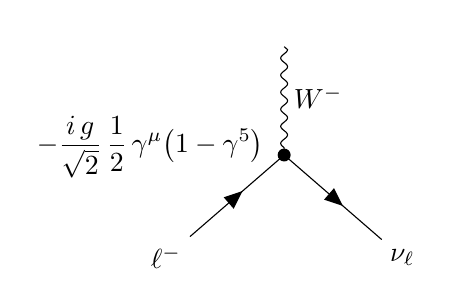
\begin{tikzpicture}
    \begin{feynman}
        % Define the central vertex and external particles
        \vertex [dot] (v) {};  % The central vertex
        \vertex [below left=1.3cm and 1.5cm of v]  (l) {\(\ell^-\)};
        \vertex [below right=1.3cm and 1.5cm of v] (n) {\(\nu_\ell\)};
        \vertex [above=1.5cm of v] (w) {};
    
        % Draw the diagram
        \diagram*{
          (l) -- [fermion] (v) -- [fermion] (n),
          (v) -- [boson, edge label'=\(W^-\)] (w),
        };
    
        % Place the vertex factor near the central vertex
        \node at ($(-1.7cm,0.1cm)$)
          {\(-\displaystyle \frac{i\,g}{\sqrt{2}} \,\frac{1}{2}\,\gamma^\mu \bigl(1-\gamma^5\bigr)\)};
    \end{feynman}
    \end{tikzpicture}
        \caption{The SM left-handed charged weak vertex.}
      \end{figure}
      \begin{itemize}
        \item Only \boldcol{UMNMaroon}{left-handed chiral} components of 
          particle spinors participate in charged weak interactions.
        \item No theoretical explanation as to \emph{why} 
          the weak force is left-handed.
      \end{itemize}
    \end{column}
    \begin{column}{0.5\textwidth}
      \begin{figure}
        \centering
        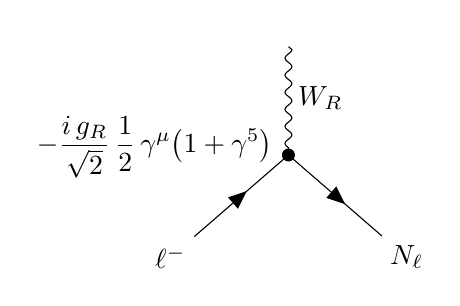
\begin{tikzpicture}
  \begin{feynman}
      % Define the central vertex and external particles
      \vertex [dot] (v) {};  % The central vertex
      \vertex [below left=1.3cm and 1.5cm of v]  (l) {\(\ell^-\)};
      \vertex [below right=1.3cm and 1.5cm of v] (n) {\(N_\ell\)};
      \vertex [above=1.5cm of v] (w) {};
  
      % Draw the diagram
      \diagram*{
        (l) -- [fermion] (v) -- [fermion] (n),
        (v) -- [boson, edge label'=\(W_{R}\)] (w),
      };
  
      % Place the vertex factor near the central vertex
      \node at ($(-1.7cm,0.1cm)$)
        {\(-\displaystyle \frac{i\,g_{R}}{\sqrt{2}} \,\frac{1}{2}\,\gamma^\mu \bigl(1+\gamma^5\bigr)\)};
  \end{feynman}
  \end{tikzpicture}
        \caption{The LRSM right-handed weak vertex.}
      \end{figure}
      \begin{itemize}
        \item Introduce $W_{R}^{\pm}$ bosons to couple to \boldcol{UMNMaroon}{right-handed chiral} components of 
        particle spinors.
        \item Parity restored as a symmetry to the standard model.
      \end{itemize}
    \end{column}
  \end{columns}
\end{frame}

\note[itemize]{
\item So when we say that the weak force is left-handed, what we mean was that the W-boson couples to
  the left-chiral component of particle spinors.
\item This can be seen in the Feynmann Diagram on the left, where we have a lepton and a neutrino coupling 
  to a Standard Model W boson. The contribution to the amplitude is given by this interaction vertex, which 
  \emph{includes} a factor of the left-chiral projection operator. This means that the W boson only couples to 
  left-chiral particle states and does not interact with right-chiral particle states.
\item But there is no theoretical reason behind this. There's nothing in the Standard Model that tells 
  us that the charged weak interaction vertex should include the left chiral projection operator, instead 
  of the right chiral projection operator, or no projection operator at all, which is the case for QED 
  and QCD. This is just something that has been determined from experiment. 
\item Left-right symmetric models add right-handed W bosons, meaning heavier W bosons that couple to the right chiral 
  component of particle spinors, and you can see that there is a factor of the right chiral projection operator at 
  the vertex.
\item And lastly, if we assume that the two coupling constants are equal to each other, then there is an explicit left-right 
  symmetry and parity is restored to the standard model.
}

\begin{frame}{Left-Right Symmetric Models}
  \begin{block}{Postulate of Left-Right Symmetric Models}
    The weak force's left-handed nature is a low energy phenomenon -- 
    the result of a broken left-right symmetry that is restored at a multi-TeV energy scale.
  \end{block}
  \vfill
  \begin{table}
    \begin{tabular}{|c|c|c|}
    \hline
    &&\\[-1em]
    ${}$ & Electroweak Standard Model & Left-Right Symmetric Model \\
    &&\\[-1em]
    \hline
    \hline
    &&\\[-1em]
    Gauge Group & $\mathrm{SU}(2)_{\mathbb{L}} \times \mathrm{U}(1)$ 
    & $\textcolor{red}{\mathrm{SU}(2)_{\mathbb{R}}} \times \mathrm{SU}(2)_\mathbb{L} 
    \times \mathrm{U}(1)$ \\ 
    &&\\[-1em]
    \hline
    &&\\[-1em]
    Fermions & 
    \(\begin{gathered}Q_{\mathbb{L}}=\left(u^i, d^i\right)_{\mathbb{L}}, 
        L_{\mathbb{L}}=\left(l^i, \nu^i\right)_{\mathbb{L}} \\ 
        Q_{\mathbb{R}}=\left(u^i, d^i\right)_{\mathbb{R}}, \quad  
        L_{\mathbb{R}}=l_{\mathbb{R}}^i\end{gathered}\) & 
        \(\begin{gathered}Q_{\mathbb{L}}=\left(u^i, d^i\right)_{\mathbb{L}}, 
        L_{\mathbb{L}}=\left(l^i, \nu^i\right)_{\mathbb{L}} \\ 
        Q_{\mathbb{R}}=\left(u^i, d^i\right)_{\mathbb{R}}, 
        L_{\mathbb{R}}=\left(l^i,\textcolor{red}{N^i}\right)_{\mathbb{R}} 
    \end{gathered}\) \\
    &&\\[-1em]
    \hline
    &&\\[-1em]
    Gauge Bosons & $W_{L}^{\pm}$, $Z$, $\gamma$ & $W_{L}^{\pm}$, 
    $\textcolor{red}{W_{R}^{\pm}}$, $Z$, $\textcolor{red}{Z^{\prime}}$ $\gamma$  \\
    \hline
\end{tabular}
    \caption{Summary of the Left-Right Symmetric SM
    with new extensions in \textcolor{red}{red}.}
  \end{table}
\end{frame}

\note[itemize]{
\item OK so to just wrap up the background here.
\item Left-right symmetric models postulate that parity violation is a low energy phenomenon, the result 
 of a broken symmetry that is restored at high energies.
\item The left-right symmetric standard model is summarized in this table, with standard model extensions 
  highlighted in red.
\item Most botably, we have extended the electroweak gauge group to include an SU(2)R symmetry group 
    in addition to the usual SU(2)L. 
\item Then, just as the left-handed fermions are doublets under SU(2)L, so too now do right-handed fermions 
  form doublets under SU(2)R.
\item Of course, we must add right-handed neutrinos to go with the right-handed leptons to form doublets
  under SU(2)R. 
\item And these right-handed fermions have charged current interactions mediated by the charged gauge bosons 
  of SU(2)R, which we can call WR±. 
\item There is also a heavy neutral boson called Z prime which also has its own, completely seperate search.
}

\begin{frame}{Feynman Diagram}
  \begin{figure}
    \centering
    \begin{tikzpicture}
    \begin{feynman}
      %
      % -- Define the incoming quarks on the left
      \vertex (qbar) at (-2, 1.5) {\(\bar{q}'\)};
      \vertex (q)    at (-2,-1.5) {\(q\)};
      
      % -- Central vertex where q qbar' -> W_R
      \vertex [dot] (wr) at (0,0) {};
      
      % -- First decay: W_R -> N_\ell + l
      \vertex [dot] (Nl) at (2.5,0) {};
      \vertex (l1)  at (4,-1.5) {\(\ell^{+}\)};
      \vertex (N) at (4, 1.5) {};
      
      % -- Second decay: N_\ell -> l + W_R
      %    Then W_R -> 2 jets
      \vertex [dot] (wrl) at (4, 1.5) {};
      \vertex (l2) at (5.5,  3) {\(\ell^{-}\)};
      \vertex (wr2) at (6,  1) {};

      %    Then W_R -> 2 jets
      \vertex [dot] (jj) at (6, 1) {};
      \vertex (jet1) at (7.5,  1.7) {jet};
      \vertex (jet2) at (7.5, 0.3) {jet};
      
      % -- Draw the diagram
      \diagram*{
        % Incoming quarks
        (qbar) -- [fermion] (wr) -- [fermion] (q),
        
        % First decay of W_R
        (wr) -- [boson, edge label=\(W_R\)] (Nl),
        (l1) -- [fermion] (Nl),
        (Nl) -- [fermion, edge label=\(N_\ell\)] (wrl),
        
        % Decay of heavy neutrino N_l
        (wrl) -- [fermion] (l2),
        (wrl) -- [boson, edge label=\(W_R^{*}\)] (wr2),

        % Decay of second W_R into jets
        (jet1) -- [fermion] (jj) -- [fermion] (jet2),
      };
    \end{feynman}
  \end{tikzpicture}
    \caption{$\mathrm{W_R}$ decay chain. 
    The final state observables are two same-flavor leptons
    and two jets.}
  \end{figure}
\end{frame}

\note[itemize]{
  \item This feynmann diagram gives us a sense of what exactly we are looking for. 
  \item We have two qaurks coming in, annihilating and producing a right-handed W. 
  That right-handed W decays to a lepton and a heavy neutrino. That heavy neutrino 
  then decays back into a same flavor lepton and an off-shell right handed W, which 
  then decays into two quarks which hadronize to jets. 
  \item So, the observable objects in the decay are two same flavor leptons, and two jets. 
}

\section{LHC and CMS}

\begin{frame}{CMS Detector at LHC}
  \begin{figure}
    \centering
    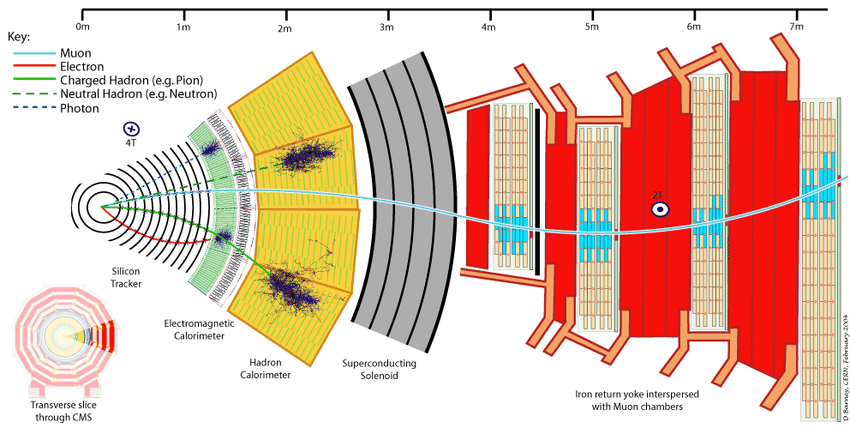
\includegraphics[width=0.85\textwidth]{../figures/experiment/cms-slice.png}
    \caption{CMS detector (slice view). Image credit -- CERN.}
  \end{figure}
\end{frame}

\note[itemize]{
  \footnotesize
  \item We search for the right-handed W using the CMS detector at the LHC.
  \item The CMS detector is a general-purpose detector, designed to improve the precision 
    of standard model measurements, as well discover any new physics that the LHC might 
    produce. It is layered like a cylindrical onion, with several concentric layers.
  \item Starting from the innermost layer is the silicon tracker, which measures the 
    trajectories of muons, electrons and charged hadrons emerging from the beam pipe. 
    The trajectories of these particles are then used to reconstruct their momentum.
  \item Beyond the tracker lie two calorimeters: the Electromagnetic Calorimeter, or 
    ECAL, which measures the energy of electrons and photons, and the Hadronic Calorimeter 
    or HCAL, which measures the energy of hadrons.
  \item  The central feature of the detector is the superconducting solenoid, which provides 
    a magnetic field of 3.8 T. The magnetic field bends the path of charged particles as they 
    traverse the detector, which in combination with the tracker allows their transverse momentum 
    to be reconstructed.
  \item In the outermost layers we have iron yoke interspersed with muon chambers. Muons are 
    not stopped by the ECAL, so we detect them and measure their energy in these outermost chambers.
}

\section{Search Strategy} % \ssection{Search Strategy}

\subsection{Resonance Searches}

\begin{frame}{Resonance Search}
  \begin{columns}
    \begin{column}{0.4\textwidth}
      \vfill
      {The cross section a \boldcol{UMNSunny}{Breit-Wigner distribution}:
      $$
        \sigma \propto \frac{1}{\left(m_{lljj}^{2} - m_{W_R}^{2}\right)^{2} + \Gamma^{2} m^{2}_{W_R}}
      $$}
      \begin{figure}
        \centering
        % Author: Izaak Neutelings (September 2022)
\usetikzlibrary{calc}
\usetikzlibrary{intersections}

% TIKZ
\tikzset{>=latex} % for LaTeX arrow head
\tikzstyle{curve}=[very thick,line cap=round]
\tikzstyle{dashed curve}=[curve,thick,dashed]
\pgfdeclarelayer{back} % to draw on background
\pgfsetlayers{back,main} % set order

% COLORS
\definecolor{myblue}{rgb}{.0,.13,.98} % 0,32,250
\definecolor{myred}{rgb}{.7,.1,.1}
\colorlet{mydarkred}{myred!80!black}
\colorlet{mydarkgreen}{green!30!black}
\colorlet{mylightgreen}{green!30!black!15}

%% FUNCTIONS
%\tikzset{declare function={% Kruskal-Szekeres coordinates
%  kruskalu(\x,\c) = {\fpeval{sqrt(\x*\x+(\c/2-1)*exp(\c/2))}};%
%}}

% DRAW RANDOM DATA POINTS
\def\yerrscale{0.26} % scale fluctuations
\def\ybarscale{0.7} % scale error bars
\def\wbar{1.2pt} % width of line at end of error bar
\def\drawdata[#1](#2:#3:#4){ % add data around named path
  \def\Ndata{#2} % number of data points 
  \pgfmathsetmacro\xmindata{#3} % xmin for graph
  \pgfmathsetmacro\xmaxdata{#4} % xmax for graph
  %\pgfmathsetmacro\wbar{0.2*\xmaxdata/\Ndata} % width of line at end of error bar
  \foreach \i [evaluate={
    \x=\xmindata+(\i-0.5)*(\xmaxdata-\xmindata)/\Ndata;
  }] in {1,...,\Ndata}{
    \message{^^J N=\Ndata, i=\i, x=\x}
    \path[name path=vline] (\x,0) -- (\x,\ymax);
    \path[name intersections={of=#1 and vline, name=i}]
      coordinate (Pdata) at ($(i-1)+(0,{0.3*(rand)/2})$);
    \fill (Pdata) circle(1.2pt);
    \draw let \p1 = (Pdata) in % calculate y coordinate
      (Pdata) --++ (0,{\ybarscale*sqrt{\y1}}) coordinate(Pup)
      (Pdata) --++ (0,{-\ybarscale*sqrt{\y1}}) coordinate(Pdn)
      (Pup)++(\wbar,0) --++ (-2*\wbar,0)
      (Pdn)++(\wbar,0) --++ (-2*\wbar,0);
  }
}

% STMET
\begin{tikzpicture}[scale=1]
  \message{^^JSTMET}
  \def\xmax{4.5} % x axis maximum
  \def\ymax{3.0} % y axis maximum
  \clip (-0.13*\xmax,-0.2*\ymax) rectangle (1.2*\xmax,1.05*\ymax);
  
  % CURVES
  \def\pathSM{
    (0,0.55*\ymax) to[out=70,in=173,looseness=1.6]
    coordinate[pos=0.8] (M)
    (0.88*\xmax,0.12*\ymax)
  }
  \fill[mylightgreen]
    (0,0) -- \pathSM |- cycle;
  \draw[curve,mydarkgreen,name path=SM]
    \pathSM;
    \begin{pgfonlayer}{back} % draw on back
        \draw[curve,myred,name path=BSM]
          (M) to[out=-30,in=140,looseness=1.7]
          (0.88*\xmax,0.28*\ymax); % <-- no node here anymore
      \end{pgfonlayer}
    
    \node at (2.9,0.25) {\textcolor{mydarkgreen}{SM}};
    \node at (3.8,1.45) {\textcolor{myred}{SM+LRSM}}; % <-- place label manually
  
  % DATA POINTS
  \drawdata[SM](11:0:0.6*\xmax)
  \drawdata[BSM](5:0.6*\xmax:0.88*\xmax)
  
  % AXES
  \draw[<->,thick]
    (\xmax,0)
    node[below left] {$m_{\ell \ell j j}$}
    -| (0,\ymax)
    node[above left,rotate=90] {Events}; 
  
\end{tikzpicture}
      \end{figure}
    \end{column}
    \begin{column}{0.59\textwidth}
      \begin{block}{Bump Huntin'}
        Search for an excess of events in the \boldcol{UMNMaroon}{four object invariant mass} 
        spectrum consisting of the two leptons and two jets ($m_{\ell \ell j j}$).
      \end{block}
      \begin{figure}
        \centering
        \resizebox{0.9\linewidth}{!}{%
          \tikzset{
  highlight/.style={draw=red, thick, circle, inner sep=2pt}
}

\begin{tikzpicture}
    \begin{feynman}
      %
      % -- Define the incoming quarks on the left
      \vertex (qbar) at (-2, 1.5) {\(q\)};
      \vertex (q)    at (-2,-1.5) {\(\bar{q}\)};
      
      % -- Central vertex where q qbar' -> W_R
      \vertex [dot] (wr) at (0,0) {};
      
      % -- First decay: W_R -> N_\ell + l
      \vertex [dot] (Nl) at (2.5,0) {};
      \vertex (l1)  at (4,-1.5) [highlight] {\(\ell\)};
      \vertex (N) at (4, 1.5) {};
      
      % -- Second decay: N_\ell -> l + W_R
      \vertex [dot] (wrl) at (4, 1.5) {};
      \vertex (l2) at (5.5,  3) [highlight] {\(\ell\)};
      \vertex (wr2) at (5.3,  0.5) {};

      %    Then W_R -> 2 jets
      \vertex [dot] (jj) at (5.3, 0.5) {};
      \vertex (jet1) at (6.5,  1.7) [highlight] {jet};
      \vertex (jet2) at (6.5, -0.5) [highlight] {jet};
      
      % -- Draw the diagram
      \diagram*{
        % Incoming quarks
        (qbar) -- [fermion] (wr) -- [fermion] (q),
        
        % First decay of W_R
        (wr) -- [boson, edge label=\(W_R\)] (Nl),
        (l1) -- [fermion] (Nl),
        (Nl) -- [fermion, edge label=\(N_\ell\)] (wrl),
        
        % Decay of heavy neutrino N_l
        (wrl) -- [fermion] (l2),
        (wrl) -- [boson, edge label=\(W_R^{*}\)] (jj),

        % Decay of second W_R into jets
        (jet1) -- [fermion] (jj) -- [fermion] (jet2),
      };
    \end{feynman}
  \end{tikzpicture}%
      }
      \end{figure}
    \end{column}
  \end{columns}
\end{frame}

\note[itemize]{
  \footnotesize
  \item The general strategy that we use to search for the right-handed W and heavy 
    neutrino is the classic resonance search, otherwise known as bump hunting. 
  \item The way that this works is we add up the four-momentum vectors of our final 
    state products and square them to get their invariant mass, which we call the 
    four-object invariant mass, or mlljj. 
  \item Then by conservation of energy and momentum, the four-object invariant mass is 
    equal to the mass of the right-handed W.
  \item This is important because the right-handed W is a propagator, and so it takes a 
    factor of 1 over mlljj squared minus mw squared in its matrix element, where mw is 
    the on shell mass. So when mlljj approaches the on shell mass of the right 
    handed w, there is a resonance in the cross section.
  \item Now if you look at this cartoon I've drawn in the bottom left you can see how 
   this appears on four object invariant mass spectrum. 
  \item The number of events on the y-axis is really just the cross section times the 
   luminosity, so this excess of events over standard model background expectations is due to this 
   resonance in the WR cross section.
  \item And I should say that the reason we favor this particular decay mode, is that we can also use this 
    same technique to measure the mass of the heavy neutrino by looking at the ljj mass spectrum. So in a 
    sense we can kill two birds with one stone by examining this particular decay mode. 
}

\begin{frame}[t]{Analysis Topologies}
  \begin{columns}[t]
    \begin{column}{0.32\textwidth}
      \centering
      \framesection{CMS Jets}
      \resizebox{0.99\linewidth}{!}{%
      % Author: Izaak Neutelings (May 2021)
% Description: hadronic top quark jet
\usetikzlibrary{calc,math,decorations.pathreplacing}

% TikZ arrow head
\tikzset{>=latex}

% COLORS
\colorlet{myblue}{blue!70!black}
\colorlet{mydarkblue}{blue!40!black}
\colorlet{mygreen}{green!40!black}
\colorlet{myred}{red!65!black}

% Cone styles
\tikzstyle{cone}     =[thin,blue!50!black,fill=blue!50!black!30]
\tikzstyle{conebase} =[cone,fill=blue!50!black!50]

% Macro to draw a jet cone from point #2 back to #1
% #1 (optional): color
% #2: apex coordinate name
% #3: base coordinate name
% #4: full opening angle (in degrees)
% #5: eccentricity factor
\newcommand\jetcone[5][blue]{{
  \pgfmathanglebetweenpoints%
    {\pgfpointanchor{#2}{center}}%
    {\pgfpointanchor{#3}{center}}%
  \edef\ang{#4/2}       % half‑opening angle
  \edef\e{#5}           % eccentricity
  \edef\vang{\pgfmathresult} % direction of axis
  \tikzmath{%
    coordinate \conevec;
    \conevec = (#2)-(#3);
    \x    = veclen(\conevecx,\conevecy)*\e*sin(\ang)^2;
    \y    = tan(\ang)*(veclen(\conevecx,\conevecy)-\x);
    \a    = veclen(\conevecx,\conevecy)*sqrt(\e)*sin(\ang);
    \b    = veclen(\conevecx,\conevecy)*tan(\ang)*sqrt(1-\e*sin(\ang)^2);
    \angb = acos(sqrt(\e)*sin(\ang));
  }
  \coordinate (tmpL) at 
    ($(#3)-(\vang:\x pt)+(\vang+90:\y pt)$);
  % Draw full ellipse for cone base
  \draw[thin,#1!40!black,rotate=\vang,
        top color=#1!50!black!80,
        bottom color=#1!40!black!80,
        shading angle=\vang]
    (#3) ellipse({\a pt} and {\b pt});
  % Draw the “cone side” as an arc + lines back to apex
  \draw[thin,#1!40!black,rotate=\vang,rounded corners=0.001pt,
        top color=#1!90!black!20,
        bottom color=#1!50!black!50,
        shading angle=\vang]
    (tmpL) arc(180-\angb:180+\angb:{\a pt} and {\b pt})
    -- (#2) -- cycle;
}}

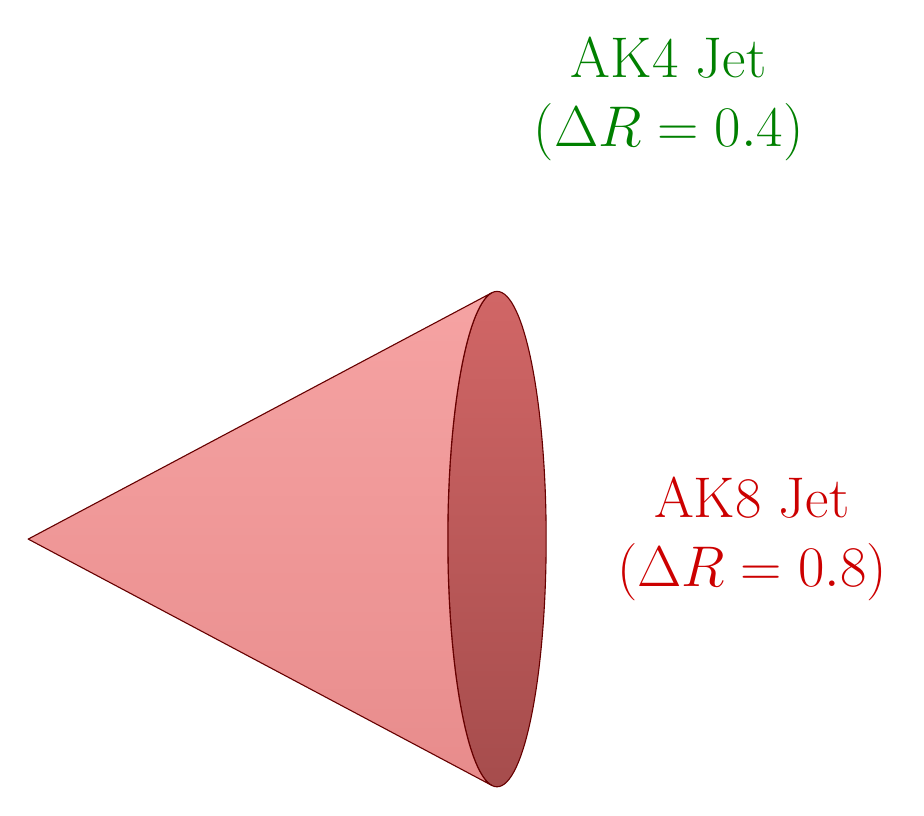
\begin{tikzpicture}[scale=7]
  % Core points
  \coordinate (O)  at (0,0);
  \coordinate (BJ) at (56:1.1);  % b‑jet axis
  \coordinate (J1) at (12:1.0);  % light q‑jet 1
  \coordinate (J2) at (-12:1.0); % light q‑jet 2
  \coordinate (M)  at (0:0.85);  % merged jet center

  % BACK of large cone
  \def\ang{28}  % full opening angle
  \def\e{0.05}  % eccentricity
  \tikzmath{%
    coordinate \axisvec;
    \axisvec = (O)-(M);
    \x    = veclen(\axisvecx,\axisvecy)*\e*sin(\ang)^2;
    \y    = tan(\ang)*(veclen(\axisvecx,\axisvecy)-\x);
    \a    = veclen(\axisvecx,\axisvecy)*sqrt(\e)*sin(\ang);
    \b    = veclen(\axisvecx,\axisvecy)*tan(\ang)*sqrt(1-\e*sin(\ang)^2);
    \angb = acos(sqrt(\e)*sin(\ang));
  }
  \coordinate (ML) at 
    ($(M)+(-180:\x pt)+(90:\y pt)$);
  % draw back half of the large cone
  \draw[thin,red!40!black,
        top color=red!70!black!60,
        bottom color=red!50!black!70]
    (M) ellipse({\a pt} and {\b pt});

  % JETS: draw three sub‑cones
  \jetcone[green!80!black]{O}{BJ}{14}{0.10} % b‑jet
  %\jetcone{O}{J1}{16}{0.08}                 % q‑jet 1
  %\jetcone{O}{J2}{16}{0.10}                 % q‑jet 2

  % Labels
  \node[green!50!black,align=center,font=\huge]
  at
    ($ (56:1.26) + (13pt,-7pt) $)
  {AK4 Jet\\$(\Delta R = 0.4)$};
  \node[red!80!black,right,align=center, font=\huge] at (0:1.05) {AK8 Jet\\$(\Delta R = 0.8)$};

  % FRONT of large cone
  \draw[thin,red!40!black,fill opacity=0.9,rounded corners=0.001pt,
        top color=red!90!black!40,
        bottom color=red!80!black!50]
    (ML) arc(180-\angb:180+\angb:{\a pt} and {\b pt})
    -- ($(O)-(0.0005,0)$) -- cycle;
\end{tikzpicture}%
      }
      {
        \footnotesize
        \begin{itemize}
          \item CMS jets are clustered with the anti $k_t$ (AK) algorithm.
          \item Jet sizes are defined in terms of the angular separation, $\left(\Delta R = \sqrt{\Delta \phi^{2} + \Delta \eta^{2}}\right)$
        \end{itemize}
      }
    \end{column}
    \begin{column}{0.32\textwidth}
      \centering
      \framesection{Resolved Region}
      \resizebox{0.99\linewidth}{!}{%
      \usetikzlibrary{calc}
\usetikzlibrary{math} % for \tikzmath
\usetikzlibrary{decorations.pathmorphing} % for snake, coil, zigzag
\tikzset{>=latex} % set default arrow head as latex

% COLORS
\colorlet{leptoncol}{green!70!black}
\colorlet{quarkcol}{blue!85!cyan!80!black}
\colorlet{photoncol}{yellow!80!orange!90!black}
\colorlet{exocol}{red!80!black}
\colorlet{anycol}{blue!80!cyan!60!red!95!black!90}

% STYLES
\tikzstyle{label}=[align=center,rounded corners=3pt] %fill=blue!60!cyan!80!black!15,
\tikzstyle{legend}=[draw=black,thick,rounded corners=3pt] %,fill=blue!60!cyan!80!black!15
\tikzstyle{entry}=[right=1pt,inner sep=4pt]
\tikzstyle{particle}=[anycol,very thick,line cap=round]
\tikzstyle{lepton}=[particle,leptoncol]
\tikzstyle{quark}=[particle,quarkcol]
\tikzstyle{track}=[quark,thick]
\tikzstyle{photon}=[particle,photoncol,decorate,decoration={
  snake,amplitude=.4mm,segment length=2.5mm,post length=1mm}]
\tikzstyle{charged exo}=[particle,exocol]
\tikzstyle{neutral exo}=[charged exo,dashed]

% JET CONE
\newcommand\jetcone[6][quarkcol]{{
  \pgfmathanglebetweenpoints
    {\pgfpointanchor{#2}{center}}
    {\pgfpointanchor{#3}{center}}%
  \pgfmathsetmacro\oang{#4/2}       % half‑opening angle
  \edef\e{#5}                       % eccentricity
  \def\tmpL{tmpL-#2-#3}             % unique coordinate name
  \edef\vang{\pgfmathresult}        % direction of axis
  \tikzmath{%
    coordinate \jetvec;             % ← was \C
    \jetvec = (#2)-(#3);            % vector OV
    \x    = veclen(\jetvecx,\jetvecy)*\e*sin(\oang)^2;
    \y    = tan(\oang)*(veclen(\jetvecx,\jetvecy)-\x);
    \a    = veclen(\jetvecx,\jetvecy)*sqrt(\e)*sin(\oang);
    \b    = veclen(\jetvecx,\jetvecy)*tan(\oang)*sqrt(1-\e*sin(\oang)^2);
    \angb = acos(sqrt(\e)*sin(\oang));
  }
  \coordinate (#2-v) at ($(#2)+(\vang:1pt)$); 
  \coordinate (\tmpL) at 
    ($(#3)-(\vang:\x pt)+(\vang+90:\y pt)$); 
  \draw[thin,#1!50!black,fill=#1!80!black!50,line cap=round,rotate=\vang]
    (#2) -- (\tmpL) arc(180-\angb:180+\angb:{\a pt} and {\b pt}) -- (#2);
  \draw[thin,#1!50!black,rotate=\vang,
        top color=#1!60!black!60,bottom color=#1!50!black!75,
        shading angle=\vang]
    (#3) ellipse({\a pt} and {\b pt});
  #6 % extra tracks
  \draw[thin,#1!50!black,rotate=\vang,fill opacity=0.80,
        top color=#1!90!black!20,bottom color=#1!50!black!50,
        line cap=round,shading angle=\vang]
    (#2) -- (\tmpL) arc(180-\angb:180+\angb:{\a pt} and {\b pt}) -- (#2);
}}

% DETECTOR
\def\scale{1.6} % scale diagrams
\def\keepseg#1#2{% % return boolean if detector segment falls outside mask
  (\mask==0 || (#2>\angmin-4 && #1<\angmax+4) || (#2>\angmin+356 && #1<\angmax+364))
}
\tikzset{
  pics/detector/.style args={#1:#2}{
    code={
  
  % MASK except segment
  \pgfmathsetmacro\mask{#1!=#2}
  \pgfmathsetmacro\angmin{#1>=0 ? #1 : 360+#1}
  \pgfmathsetmacro\angmax{#2>=0 ? #2 : 360+#2}
  \message{^^JDetector: 1=#1, 2=#2, angmin=\angmin, angmax=\angmax, mask=\mask}
  \begin{scope}[pic actions]
  
  % CLIP
  \ifnum\mask=1 % clip detector segment
    %\draw[thick,black] (0,0) -- (#1:2.3) arc(#1:#2:2.3) -- cycle;
    %\clip (0,0) -- (\angmin:2.3) arc(\angmin:\angmax:2.3) -- cycle;
    \clip (0,0) -- (#1:2.3) arc(#1:#2:2.3) -- cycle;
  \fi
  
  % PIXEL TRACKER (PBIX)
  \foreach \Rlay in {0.09,0.13,0.17,0.21}{
    \message{^^JPixel tracker: Rlay=\Rlay}
    \draw[line width=0.1] (0,0) circle(\Rlay);
  }
  
  % SILICON INNER TRACKER (TIB)
  \def\h{0.12}
  \def\w{0.010}
  \def\d{0.028}
  \foreach \Rlay/\Nlay in {0.40/30,0.55/38,0.70/46,0.85/52}{
    \message{^^JInner tracker: Rlay=\Rlay, Nlay=\Nlay}
    \foreach \i [
      evaluate={\ang=\i*(360/\Nlay);\keep=\keepseg{\ang}{\ang};}
    ] in {1,...,\Nlay}{
      \ifnum\keep=1
        \fill[rotate around={\ang+10:(\ang:\Rlay-\d)},rounded corners=0.05pt]
          (\ang:\Rlay-\d)++(-\w/2,-\h/2) rectangle++(\w,\h);
        \fill[rotate around={\ang+10:(\ang:\Rlay+\d)},rounded corners=0.05pt]
          (\ang:\Rlay+\d)++(-\w/2,-\h/2) rectangle++(\w,\h);
      \fi
    }
  }
  
  % OUTER TRACKER (TOB)
  \def\h{0.18}
  \def\w{0.011}
  \def\d{0.021}
  \foreach \Rlay/\Nlay in {1.00/21,1.12/24,1.24/27,1.36/30,1.48/33,1.64/37}{
    \message{^^JOuter tracker: Rlay=\Rlay, Nlay=\Nlay}
    \foreach \i [
      evaluate={\anga=(\i-1)*360/\Nlay;\angb=(\i-0.5)*360/\Nlay;
                \keep=\keepseg{\anga}{\angb};}
    ] in {1,...,\Nlay}{
      \ifnum\keep=1
        \fill[rotate={\anga},rounded corners=0.05pt]
          (0:\Rlay-\d-0.55*\w)++(-\w/2,-\h/2) rectangle++(\w,\h)
          (0:\Rlay-\d+0.55*\w)++(-\w/2,-\h/2) rectangle++(\w,\h);
        \fill[rotate={\angb},rounded corners=0.1pt]
          (0:\Rlay+\d-0.55*\w)++(-\w/2,-\h/2) rectangle++(\w,\h)
          (0:\Rlay+\d+0.55*\w)++(-\w/2,-\h/2) rectangle++(\w,\h);
      \fi
    }
  }
  
  % ECAL
  \def\Ntow{18}
  \def\Rin{1.85} % inner radius
  \def\Rout{2.24} % outer radius
  \message{^^JECAL: Ntow=\Ntow}
  \foreach \i [
      evaluate={\anga=(\i-1.5)*360/\Ntow;\angb=(\i-0.5)*360/\Ntow;
                \keep=\keepseg{\anga}{\angb};}
    ] in {1,...,\Ntow}{
      \ifnum\keep=1
        \draw (\anga:\Rin) -- (\anga:\Rout) --
              (\angb:\Rout) -- (\angb:\Rin) -- cycle;
      \fi
  }
  
  %% HCAL
  %\def\Rin{2.28} % inner radius
  %\def\Rout{3.8} % outer radius
  %\message{^^JHCAL: Ntow=\Ntow}
  %\foreach \i [
  %    evaluate={\anga=(\i-1.5)*360/\Ntow;\angb=(\i-0.5)*360/\Ntow;}
  %  ] in {1,...,\Ntow}{
  %  \draw
  %    (\anga:\Rin) -- (\anga:\Rout) --
  %    (\angb:\Rout) -- (\angb:\Rin) -- cycle;
  %}
  
  \end{scope}
  \ifnum\mask=1
    \draw[black!30] (\angmax:2.5) -- (0,0) -- (\angmin:2.5);
  \fi
    
    }
  },
  pics/detector/.default={0:0}
}

\begin{tikzpicture}[scale=5*\scale,
    rotate=0, 
    every node/.style={font=\fontsize{48}{14}\selectfont},
    % (you can still override per-path if needed)
]
  \def\angN{-162} % angle of HNL
  \def\lang{-100} % angle of HNL
  \def\dang{270} % angle of HNL
  \draw pic[black!15,scale=5*\scale] {detector={180:\dang}}; % \draw pic[black!15,scale=\scale] {detector={180:\dang}};
  \coordinate (PV) at (0,0); % primary vertex
  \draw[neutral exo, very thick] (PV) -- (\angN:0.90) coordinate (V)
    node[pos=0.7,above=0pt] {$\mathrm{N}$};
  \coordinate (J1) at (\angN+5:2.34); % displaced jet vector
  \coordinate (J2) at (\angN+40:2.00); % displaced jet vector
  \coordinate (L1) at (\lang:2.50);  % prompt lepton \coordinate (L1) at (\lang:2.50); 
  \coordinate (L2) at (\angN-16:2.69); % displaced lepton
  \draw[->,lepton, very thick] (PV) to[bend right=13] (L1) % prompt lepton
    node[anchor=172+\lang,inner sep=1pt] {$\ell$};

  \jetcone[quarkcol]{V}{J1}{23}{0.12}{ % displaced jet
    \draw[->,track, very thick] (V-v) to[bend right=9] (\angN+10:2.60);
    \draw[->,track,dashed, very thick] (V-v) -- (\angN+4:2.63);
    \draw[->,track, very thick] (V-v) to[bend left=8] (\angN-2:2.62);
  }

  \draw[->,lepton, very thick] (V-v) to[bend right=14] (L2) % displaced lepton
  node[anchor=40,inner sep=0pt] {$\ell$};

  \jetcone[quarkcol]{V}{J2}{20}{0.12}{ % displaced jet
    \draw[->,track, very thick] (V-v) to[bend left=8] (\angN+36:2.52);
    \draw[->,track,dashed, very thick] (V-v) -- (\angN+45:2.53);
    \draw[->,track, very thick] (V-v) to[bend right=7] (\angN+53:2.50);
  }
\end{tikzpicture}%
      }
      {
        \footnotesize
        \begin{itemize}
          \item $m_{N} > 0.1 m_{W_{R}}$
          \item Four isolated objects: two leptons and two AK4 jets.
          \item Signal in four-object mass spectrum $m_{\ell \ell j j}$.
        \end{itemize}
      }
    \end{column}
    \begin{column}{0.32\textwidth}
      \centering
      \framesection{Boosted Region}
      \resizebox{0.99\linewidth}{!}{%
      \usetikzlibrary{calc}
\usetikzlibrary{math} % for \tikzmath
\usetikzlibrary{decorations.pathmorphing} % for snake, coil, zigzag
\tikzset{>=latex} % set default arrow head as latex

% COLORS
\colorlet{leptoncol}{green!70!black}
\colorlet{quarkcol}{blue!85!cyan!80!black}
\colorlet{photoncol}{yellow!80!orange!90!black}
\colorlet{exocol}{red!80!black}
\colorlet{anycol}{blue!80!cyan!60!red!95!black!90}

% STYLES
\tikzstyle{label}=[align=center,rounded corners=3pt] %fill=blue!60!cyan!80!black!15,
\tikzstyle{legend}=[draw=black,thick,rounded corners=3pt] %,fill=blue!60!cyan!80!black!15
\tikzstyle{entry}=[right=1pt,inner sep=4pt]
\tikzstyle{particle}=[anycol,very thick,line cap=round]
\tikzstyle{lepton}=[particle,leptoncol]
\tikzstyle{quark}=[particle,quarkcol]
\tikzstyle{track}=[quark,thick]
\tikzstyle{photon}=[particle,photoncol,decorate,decoration={
  snake,amplitude=.4mm,segment length=2.5mm,post length=1mm}]
\tikzstyle{charged exo}=[particle,exocol]
\tikzstyle{neutral exo}=[charged exo,dashed]

% JET CONE
\newcommand\jetcone[6][quarkcol]{{
  \pgfmathanglebetweenpoints
    {\pgfpointanchor{#2}{center}}
    {\pgfpointanchor{#3}{center}}%
  \pgfmathsetmacro\oang{#4/2}       % half‑opening angle
  \edef\e{#5}                       % eccentricity
  \def\tmpL{tmpL-#2-#3}             % unique coordinate name
  \edef\vang{\pgfmathresult}        % direction of axis
  \tikzmath{%
    coordinate \jetvec;             % ← was \C
    \jetvec = (#2)-(#3);            % vector OV
    \x    = veclen(\jetvecx,\jetvecy)*\e*sin(\oang)^2;
    \y    = tan(\oang)*(veclen(\jetvecx,\jetvecy)-\x);
    \a    = veclen(\jetvecx,\jetvecy)*sqrt(\e)*sin(\oang);
    \b    = veclen(\jetvecx,\jetvecy)*tan(\oang)*sqrt(1-\e*sin(\oang)^2);
    \angb = acos(sqrt(\e)*sin(\oang));
  }
  \coordinate (#2-v) at ($(#2)+(\vang:1pt)$); 
  \coordinate (\tmpL) at 
    ($(#3)-(\vang:\x pt)+(\vang+90:\y pt)$); 
  \draw[thin,#1!50!black,fill=#1!80!black!50,line cap=round,rotate=\vang]
    (#2) -- (\tmpL) arc(180-\angb:180+\angb:{\a pt} and {\b pt}) -- (#2);
  \draw[thin,#1!50!black,rotate=\vang,
        top color=#1!60!black!60,bottom color=#1!50!black!75,
        shading angle=\vang]
    (#3) ellipse({\a pt} and {\b pt});
  #6 % extra tracks
  \draw[thin,#1!50!black,rotate=\vang,fill opacity=0.80,
        top color=#1!90!black!20,bottom color=#1!50!black!50,
        line cap=round,shading angle=\vang]
    (#2) -- (\tmpL) arc(180-\angb:180+\angb:{\a pt} and {\b pt}) -- (#2);
}}

% DETECTOR
\def\scale{1.6} % scale diagrams
\def\keepseg#1#2{% % return boolean if detector segment falls outside mask
  (\mask==0 || (#2>\angmin-4 && #1<\angmax+4) || (#2>\angmin+356 && #1<\angmax+364))
}
\tikzset{
  pics/detector/.style args={#1:#2}{
    code={
  
  % MASK except segment
  \pgfmathsetmacro\mask{#1!=#2}
  \pgfmathsetmacro\angmin{#1>=0 ? #1 : 360+#1}
  \pgfmathsetmacro\angmax{#2>=0 ? #2 : 360+#2}
  \message{^^JDetector: 1=#1, 2=#2, angmin=\angmin, angmax=\angmax, mask=\mask}
  \begin{scope}[pic actions]
  
  % CLIP
  \ifnum\mask=1 % clip detector segment
    %\draw[thick,black] (0,0) -- (#1:2.3) arc(#1:#2:2.3) -- cycle;
    %\clip (0,0) -- (\angmin:2.3) arc(\angmin:\angmax:2.3) -- cycle;
    \clip (0,0) -- (#1:2.3) arc(#1:#2:2.3) -- cycle;
  \fi
  
  % PIXEL TRACKER (PBIX)
  \foreach \Rlay in {0.09,0.13,0.17,0.21}{
    \message{^^JPixel tracker: Rlay=\Rlay}
    \draw[line width=0.1] (0,0) circle(\Rlay);
  }
  
  % SILICON INNER TRACKER (TIB)
  \def\h{0.12}
  \def\w{0.010}
  \def\d{0.028}
  \foreach \Rlay/\Nlay in {0.40/30,0.55/38,0.70/46,0.85/52}{
    \message{^^JInner tracker: Rlay=\Rlay, Nlay=\Nlay}
    \foreach \i [
      evaluate={\ang=\i*(360/\Nlay);\keep=\keepseg{\ang}{\ang};}
    ] in {1,...,\Nlay}{
      \ifnum\keep=1
        \fill[rotate around={\ang+10:(\ang:\Rlay-\d)},rounded corners=0.05pt]
          (\ang:\Rlay-\d)++(-\w/2,-\h/2) rectangle++(\w,\h);
        \fill[rotate around={\ang+10:(\ang:\Rlay+\d)},rounded corners=0.05pt]
          (\ang:\Rlay+\d)++(-\w/2,-\h/2) rectangle++(\w,\h);
      \fi
    }
  }
  
  % OUTER TRACKER (TOB)
  \def\h{0.18}
  \def\w{0.011}
  \def\d{0.021}
  \foreach \Rlay/\Nlay in {1.00/21,1.12/24,1.24/27,1.36/30,1.48/33,1.64/37}{
    \message{^^JOuter tracker: Rlay=\Rlay, Nlay=\Nlay}
    \foreach \i [
      evaluate={\anga=(\i-1)*360/\Nlay;\angb=(\i-0.5)*360/\Nlay;
                \keep=\keepseg{\anga}{\angb};}
    ] in {1,...,\Nlay}{
      \ifnum\keep=1
        \fill[rotate={\anga},rounded corners=0.05pt]
          (0:\Rlay-\d-0.55*\w)++(-\w/2,-\h/2) rectangle++(\w,\h)
          (0:\Rlay-\d+0.55*\w)++(-\w/2,-\h/2) rectangle++(\w,\h);
        \fill[rotate={\angb},rounded corners=0.1pt]
          (0:\Rlay+\d-0.55*\w)++(-\w/2,-\h/2) rectangle++(\w,\h)
          (0:\Rlay+\d+0.55*\w)++(-\w/2,-\h/2) rectangle++(\w,\h);
      \fi
    }
  }
  
  % ECAL
  \def\Ntow{18}
  \def\Rin{1.85} % inner radius
  \def\Rout{2.24} % outer radius
  \message{^^JECAL: Ntow=\Ntow}
  \foreach \i [
      evaluate={\anga=(\i-1.5)*360/\Ntow;\angb=(\i-0.5)*360/\Ntow;
                \keep=\keepseg{\anga}{\angb};}
    ] in {1,...,\Ntow}{
      \ifnum\keep=1
        \draw (\anga:\Rin) -- (\anga:\Rout) --
              (\angb:\Rout) -- (\angb:\Rin) -- cycle;
      \fi
  }
  
  %% HCAL
  %\def\Rin{2.28} % inner radius
  %\def\Rout{3.8} % outer radius
  %\message{^^JHCAL: Ntow=\Ntow}
  %\foreach \i [
  %    evaluate={\anga=(\i-1.5)*360/\Ntow;\angb=(\i-0.5)*360/\Ntow;}
  %  ] in {1,...,\Ntow}{
  %  \draw
  %    (\anga:\Rin) -- (\anga:\Rout) --
  %    (\angb:\Rout) -- (\angb:\Rin) -- cycle;
  %}
  
  \end{scope}
  \ifnum\mask=1
    \draw[black!30] (\angmax:2.5) -- (0,0) -- (\angmin:2.5);
  \fi
    
    }
  },
  pics/detector/.default={0:0}
}

\begin{tikzpicture}[scale=3.6*\scale,
    rotate=0, 
    every node/.style={font=\fontsize{36}{14}\selectfont},
    % (you can still override per-path if needed)
]
  \def\angN{-155} % angle of HNL
  \def\lang{-110} % angle of HNL
  \def\dang{270} % angle of HNL
  \draw pic[black!15,scale=3.6*\scale] {detector={180:\dang}}; % \draw pic[black!15,scale=\scale] {detector={180:\dang}};
  \coordinate (PV) at (0,0); % primary vertex
  \draw[neutral exo, very thick] (PV) -- (\angN:0.90) coordinate (V)
    node[pos=0.7,above=0pt] {$\mathrm{N}$};
  \coordinate (J) at (\angN+5:2.34); % displaced jet vector
  \coordinate (L1) at (\lang:2.50);  % prompt lepton \coordinate (L1) at (\lang:2.50); 
  \coordinate (L2) at (\angN-16:2.69); % displaced lepton
  \draw[->,lepton, very thick] (PV) to[bend right=13] (L1) % prompt lepton
    node[anchor=172+\lang,inner sep=1pt] {$\ell$};

  \jetcone[photoncol]{V}{J}{40}{0.12}{ % displaced jet 0.12
    \draw[->,track, very thick] (V-v) to[bend right=9] (\angN+7:2.60);
    \draw[->,track,dashed, very thick] (V-v) -- (\angN+4:2.63);
    \draw[->,track, very thick] (V-v) to[bend left=8] (\angN-2:2.62);
    \draw[->,lepton, very thick] (V-v) to[bend right=14] ((\angN+10:2.61) % displaced lepton
  node[anchor=40,inner sep=0pt] {$\ell$};
  }
\end{tikzpicture}%
      }
      {
        \footnotesize
        \begin{itemize}
          \item $m_{N} < 0.1 m_{W_{R}}$
          \item Two isolated objects: one lepton and one AK8 jet.
          \item Signal in di-object mass spectrum $m_{\ell J}$.
        \end{itemize}
      }
    \end{column}
  \end{columns}
\end{frame}

\note[itemize]{
  \footnotesize
  \item So when one of our final state quarks hadronizes, it produces a shower of particles that 
    pass through the CMS detector in a narrow cone. Rather than trying to track the energy and 
    momentum of each one of those particles, CMS clusters these particles together using something 
    called the anti kt algorithm and calls the collection of those particles a jet and we look at 
    the energy and momenta of that object as a whole.
  \item The sizes of these jets are defined in terms of the angular separation or angular distance 
    $\Delta R$, which is a measure of how collimated the particles in a jet are. The two most common 
    jet sizes are $\Delta R = 0.4$ and $\Delta R = 0.8$.
  \item There are two regions in the analysis, and so far I have only discussed this first one, the 
    resolved region. In the resolved search, we are searching for four isolated objects: two leptons, which
    I have drawn in green here, and two ak4 jets which are these blue cones. And we search for signal 
    in the four object invariant mass spectrum.
  \item But, there is another region called the boosted region. This occurs when the mass of the 
    right-handed W is much greater than the mass the heavy neutrino. Then, when the WR decays, the heavy 
    neutrino will be produced with a large momentum, and then the three decay predicts of the heavy 
    neutrino will be highly collimated as they pass through the detector. So then rather than try to 
    reconstruct each of these objects individually, we cluster them into an AK8 jet, which we also call 
    a fat jet.
  \item So then in the boosted region, we have two objects: a well isolated lepton shown here in green, 
    and the neutrino decay products, which we reconstruct as a fat jet. We then use the invariant mass 
    of these two objects to search for signal.
  \item But for the rest of this talk, I am only going to focus on the resolved region. 
}

\begin{frame}{Analysis Backgrounds}
  \begin{block}{Dominant Backgrounds}
    The two main backgrounds that result in an $\ell \ell j j$ final state are 
    \boldcol{UMNMaroon}{Drell-Yan (DY)} and \boldcol{UMNMaroon}{$\mathbf{t\bar{t}}$}.
  \end{block}
  \vfill
  \begin{columns}
    \begin{column}{0.5\textwidth}
      \begin{figure}
        \centering
        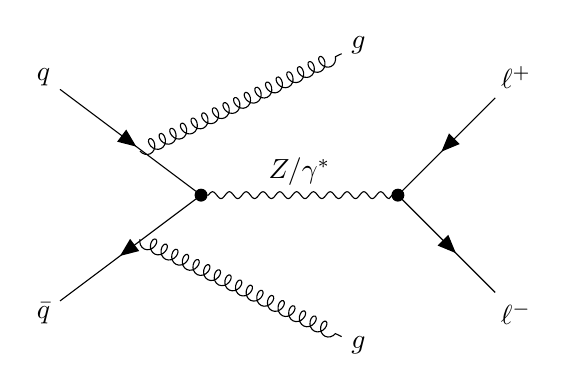
\begin{tikzpicture}
    \begin{feynman}
      % — External particle labels
      \vertex (qbar) at (-2,  1.5) {\(q\)};
      \vertex (q)    at (-2, -1.5) {\(\bar{q}\)};
      \vertex (l1)   at ( 4, -1.5) {\(\ell^{-}\)};
      \vertex (l2)   at ( 4,  1.5) {\(\ell^{+}\)};
  
      % — “Radiation” vertices on the incoming lines
      \vertex (r1) at (-0.9,  0.5) {};
      \vertex (r2) at (-0.9, -0.5) {};
  
      % — Gluon endpoints (you can label or style these as you like)
      \vertex (gl1)  at (2,  1.9) {\(g\)};
      \vertex (gl2)  at (2, -1.9) {\(g\)};
  
      % — Central Z‐decay vertices
      \vertex [dot] (Z)  at (0, 0) {};
      \vertex [dot] (ll) at (2.5, 0) {};
  
      % — Main diagram (fermions + Z → ℓ⁺ℓ⁻)
      \diagram*{
        (qbar) -- [fermion] (Z) -- [fermion] (q),
        (Z)    -- [boson, edge label=$Z/\gamma^{*}$] (ll),
        (ll)   -- [fermion] (l1),
        (l2)   -- [fermion] (ll),
      };
  
      % — Gluon radiation off each quark line
      \draw [gluon] (r1) to (gl1);
      \draw [gluon] (r2) to (gl2);
    \end{feynman}
  \end{tikzpicture}
        \caption{The Drell-Yan (DY) process.}
      \end{figure}
    \end{column}
    \begin{column}{0.5\textwidth}
      \begin{figure}
        \centering
        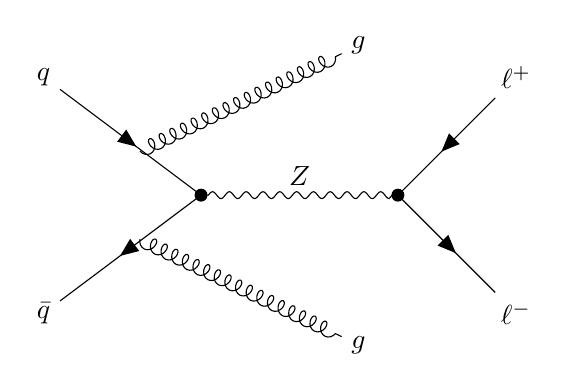
\begin{tikzpicture}
    \begin{feynman}
      % — External particle labels
      \vertex (qbar) at (-2,  1.5) {\(q\)};
      \vertex (q)    at (-2, -1.5) {\(\bar{q}\)};
      \vertex (l1)   at ( 4, -1.5) {\(\ell^{-}\)};
      \vertex (l2)   at ( 4,  1.5) {\(\ell^{+}\)};
  
      % — “Radiation” vertices on the incoming lines
      \vertex (r1) at (-0.9,  0.5) {};
      \vertex (r2) at (-0.9, -0.5) {};
  
      % — Gluon endpoints (you can label or style these as you like)
      \vertex (gl1)  at (2,  1.9) {\(g\)};
      \vertex (gl2)  at (2, -1.9) {\(g\)};
  
      % — Central Z‐decay vertices
      \vertex [dot] (Z)  at (0, 0) {};
      \vertex [dot] (ll) at (2.5, 0) {};
  
      % — Main diagram (fermions + Z → ℓ⁺ℓ⁻)
      \diagram*{
        (qbar) -- [fermion] (Z) -- [fermion] (q),
        (Z)    -- [boson, edge label=\(Z\)] (ll),
        (ll)   -- [fermion] (l1),
        (l2)   -- [fermion] (ll),
      };
  
      % — Gluon radiation off each quark line
      \draw [gluon] (r1) to (gl1);
      \draw [gluon] (r2) to (gl2);
    \end{feynman}
  \end{tikzpicture}
        \caption{$\mathrm{t\bar{t}}$ decay.}
      \end{figure}
    \end{column}
  \end{columns}
  \centering
  \boldcol{UMNSunny}{Minor Backgrounds include W+Jets, Single Top, Diboson, Triboson}
\end{frame}

\note[itemize]{
\item Of course, in order to be able to observe any signal events, you have to know your backgrounds extremely
  well. 
\item The two main backgrounds that result in a two lepton two jet final state are drell-yan and tt bar.
\item In Drell-yan events we have qq bar annhilation producing a Z or a photon, which decays to two leptons,
  and we get two jets from ISR or FSR radiation. 
\item In ttbar, if you look at this top quark here, the top quark decays to a bottom and a W, and the W decays 
  to a lepton and a neutrino. And a similar thing with the anti top quark. So in tt bar events we also have a 
  two lepton and two jet final state. 
\item A major difference between them that I want to point out is that with drell-yan events, the leptons are 
  constrained to have the same-flavor. Whereas with ttbar events, the top quarks decay independently, so the leptons 
  can have different flavors. And we are going to use this to our advantage in the next couple of slides here.
  }

\subsection{Analysis Regions}

\begin{frame}{Analysis Regions}
  \begin{figure}
    \centering
    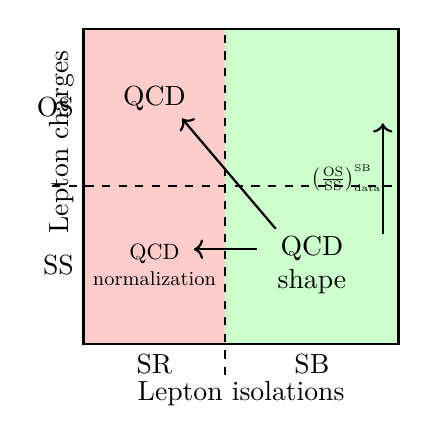
\begin{tikzpicture}[scale=4]
  
    \def\mx{0.45} %middle
    
    % boxes
    \fill [red!20!white] % SR
      (0,0) rectangle (\mx,1);
    \fill [green!20!white] % SB
      (\mx,0) rectangle (1,1);
    \draw[thick]
      (0,0) rectangle (1,1);
    
    % dashed lines
    \draw[dashed,thick]
      (\mx,-0.1) -- (\mx,1);
    \draw[dashed,thick]
      (-0.1,0.5) -- (1,0.5);
    
    % labels
    \draw
      (0,0.75) node[anchor=east]  {OS}
      (0,0.25) node[anchor=east]  {SS}
      (\mx/2,0) node[anchor=north] {SR}
      (0.5+\mx/2,0) node[anchor=north] {SB}
      (0,0.50) node[rotate=90,above=16pt] {Lepton charges}
      (0.50,0) node[below=10pt] {Lepton isolations};
    \draw
      (\mx/2,0.78) node {QCD}
      (0.5+\mx/2,0.25) node[align=center] {QCD\\shape} %{$\text{QCD}^\text{SS,SB}_\text{data}$};
      (\mx/2,0.25) node[align=center,scale=0.80] {QCD\\\small normalization};
    
    % arrows
    \draw[->,thick] % SR: SS -> OS
      (\mx+0.1,0.30) -- (\mx-0.1,0.30);
      %node[midway,above=8pt,right=-2pt,scale=0.70]{};
    \draw[->,thick] % SB: SS -> OS
      (0.95,0.35) -- (0.95,0.7)
      node[midway,above=8pt,left=-2pt,scale=0.70]{$\left(\frac{\text{OS}}{\text{SS}}\right)^\text{\tiny SB}_\text{\tiny data}$};
    
    \begin{scope}[shift={(\mx+0.02,0.54)},scale=0.35]
      \draw[->,thick]
        (0.40,-0.5) -- (-0.45,0.5);
        %node[midway,above=5pt,right=0pt,scale=0.8]{ $F^{\tiny \text{e}\mu}_\text{\tiny sim}$};
    \end{scope}
    
  \end{tikzpicture}
    \caption{A schematic diagram of the analysis region. The DY background is estimated from 
    the DY CR (blue).The backgrounds from $tW$ and $t\bar{t}$ production are estimated from the flavor CR 
    (green), where opposite flavor (OF) leptons are require.}
    \label{fig:dm-mass-scale}
  \end{figure}
\end{frame}

\note[itemize]{
  \item We estimate our backgrounds with Monte Carlo simulation, and we define these different regions of
    phase space in order to help simulate our backgrounds and derive corrections to them. 
  \item Starting in the top right corner is the signal region. In our signal region we have two same flavor leptons,
    so two electrons or two muons, and on the x-axis is the dilepton invariant mass. So, we
    require in the signal region that the invariant mass of the dileptons be considerably high, above 400 GeV.
    We do this in order to reduce our backgrounds.
  \item If we go to the left on the x-axis, between 60 and 150 GeV is our Drell-Yan control region. The Z peak
    is located here at about 91 GeV, so this area is dominated by Drell-Yan background. So we define our Drell
    Yan control region here to derive corrections to our Drell-Yan Monte Carlo.
  \item Lastly, in our flavor control region we have the same 400 GeV dilepton mass requirement that we have 
    in the signal region, but now we require two opposite flavor leptons, so one electron and one muon. 
  \item This region is dominated by ttbar decay, and we have no Drell-Yan or signal in this region, so we use 
    this region to derive corrections to our ttbar background.
}

\section{Background Estimation}

\begin{frame}{Signal Region Backgrounds}
  \begin{columns}
    \begin{column}{0.50\textwidth}
      \centering
      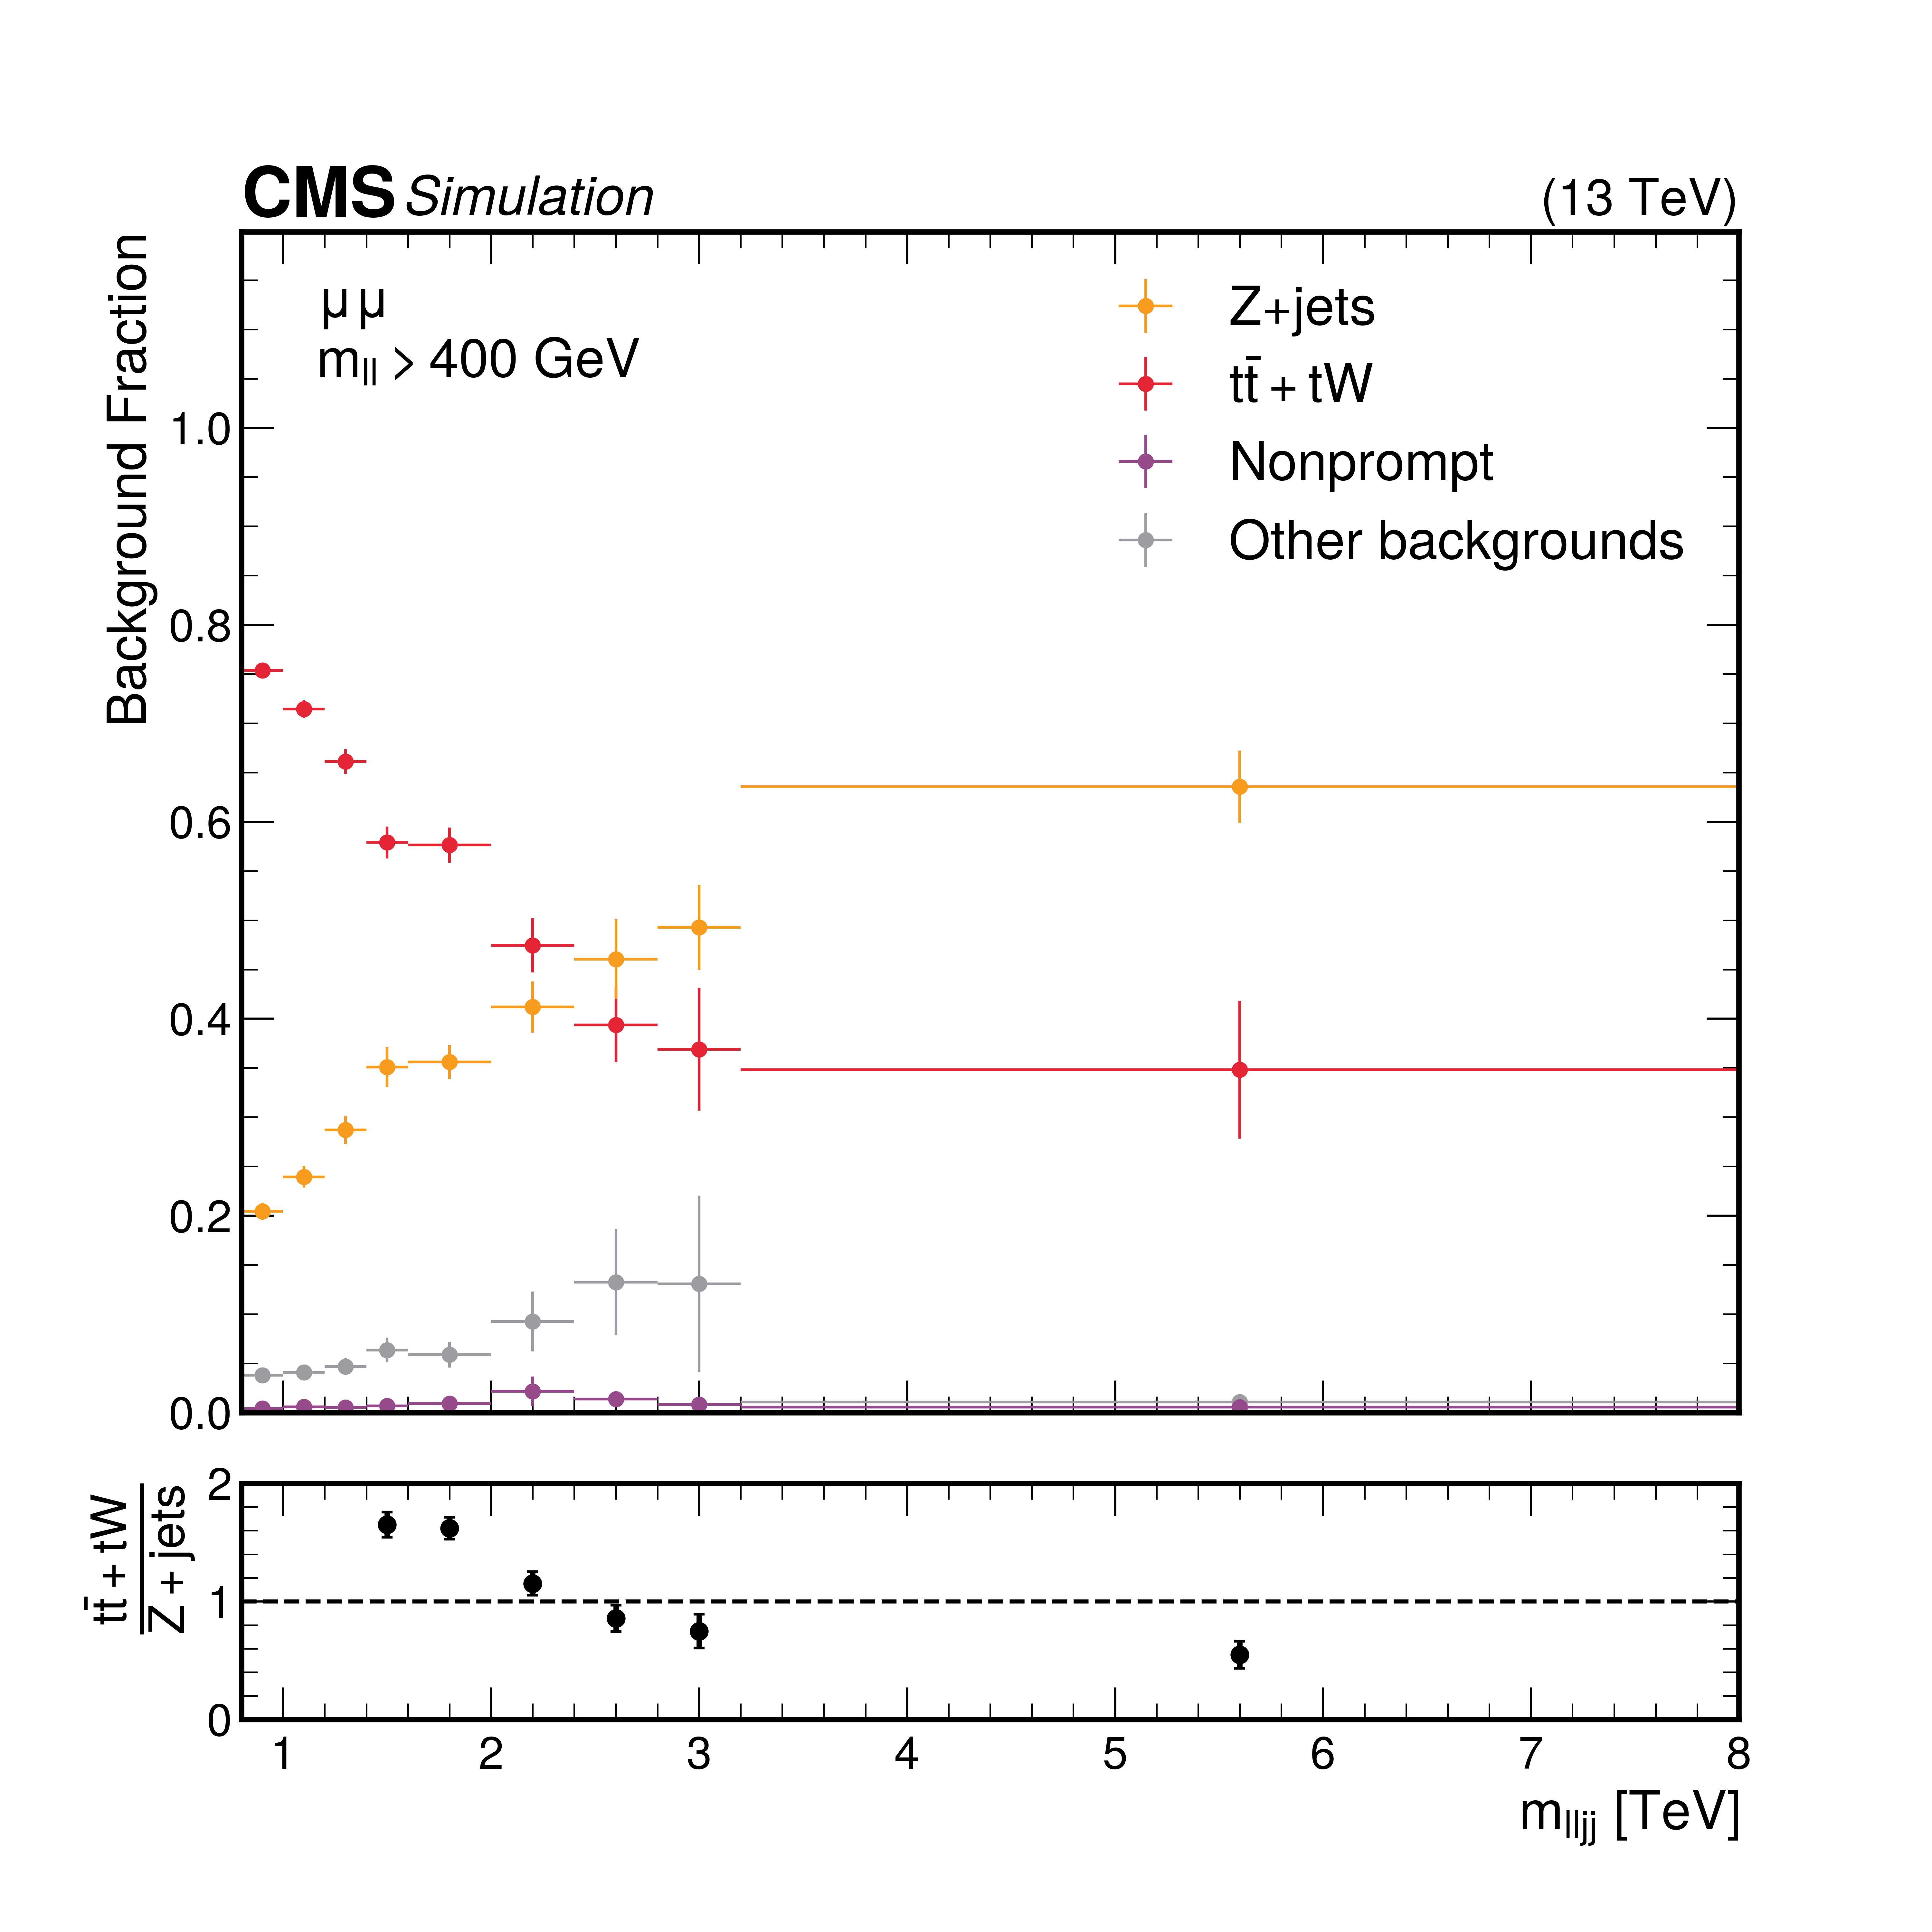
\includegraphics[width=\textwidth]{../figures/plots/sr-bkg-frac-mumu.png}
    \end{column}
    \begin{column}{0.50\textwidth}
        \vspace*{-15mm}
        \centering
        \resizebox{\columnwidth}{!}{%
        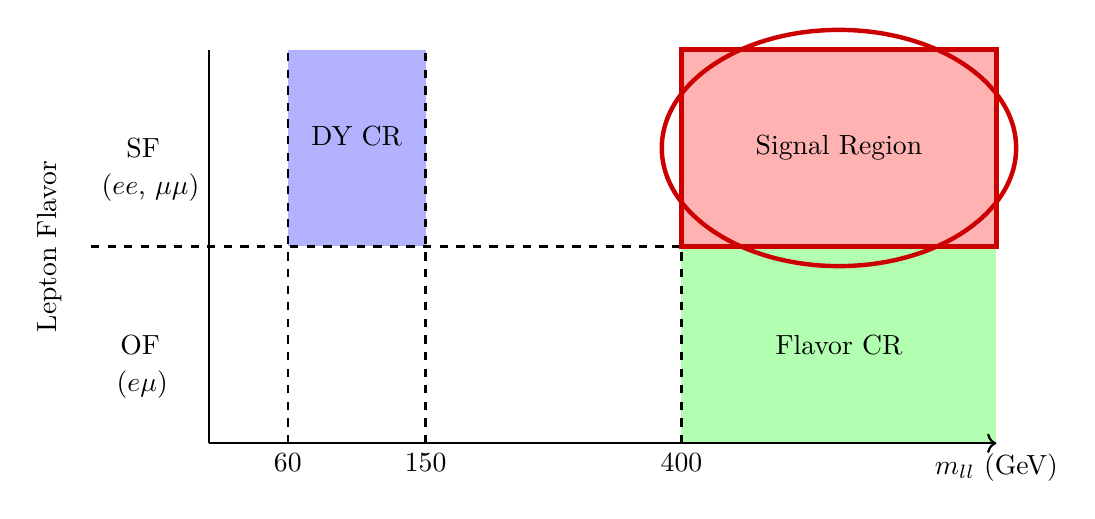
\begin{tikzpicture}[scale=5]
  
    % Define the division points for the vertical regions
    \def\xzero{0.2}   % New left margin division (empty or used for spacing)
    \def\xone{0.55}   % Right boundary of region 1 (DYCR)
    \def\xtwo{1.2}   % Right boundary of region 2 (CR)/left boundary of region 3 (SB)
    \def\xmax{2}      % Overall width of the box

    % -- Fill each grid cell with distinct colors --
    % Column 1: between xzero and xone
    \fill [blue!30!white]    (\xzero,0.5) rectangle (\xone,1);   % Top cell
    \fill [white]    (\xzero,0) rectangle (\xone,0.5);      % Bottom cell

    % Column 2: between xone and xtwo
    \fill [white]   (\xone,0.5) rectangle (\xtwo,1);       % Top cell
    \fill [white]   (\xone,0) rectangle (\xtwo,0.5);         % Bottom cell

    % Column 3: between xtwo and xmax
    \fill [red!30!white]  (\xtwo,0.5) rectangle (\xmax,1);         % Top cell
    \fill [green!30!white]  (\xtwo,0) rectangle (\xmax,0.5);           % Bottom cell
      
    % -- Draw dashed vertical division lines --
    \draw[dashed,thick] (\xzero,0) -- (\xzero,1);  % New left margin boundary
    \draw[dashed,thick] (\xone,0) -- (\xone,1);
    \draw[dashed,thick] (\xtwo,0) -- (\xtwo,1);
    
    % -- Draw a horizontal dashed line (dividing the rows) --
    \draw[dashed,thick] (-0.3,0.5) -- (\xmax,0.5);
    
    % -- Label the y-axis regions (lepton charges) --
    \draw
      (-0.1,0.75) node[anchor=east] {SF}
      (0,0.65) node[anchor=east] {($ee$, $\mu\mu$)}
      (-0.1,0.25) node[anchor=east] {OF}
      (-0.08,0.15) node[anchor=east] {($e\mu$)};
    
    % -- Label the x-axis tick marks (using the original vertical lines) --
    \draw
      (\xzero,0) node[anchor=north] {60}
      (\xone,0) node[anchor=north] {150}
      (\xtwo,0) node[anchor=north] {400};
    
    % -- Axis description on the left --
    \draw
      (-0.35,0.5) node[rotate=90,anchor=south] {Lepton Flavor};
    
    % -- Draw the x-axis as an arrow along the bottom edge --
    \draw[->, thick] (0,0) -- (\xmax,0) node[anchor=north] {$m_{ll}$ (GeV)};
    
    % -- Optionally draw the y-axis line --
    \draw[thick] (0,0) -- (0,1);

    % -- Add internal region labels --
    % Place the label for the DYCR region at the center of the first (red) column:
    \draw ({(\xzero+\xone)/2},0.78) node {DY CR};
    % Place the label for the CR region in the center of the second (blue) column (here using the bottom half for example):
    \draw ({\xtwo+(\xmax-\xtwo)/2},0.25) node[align=center] {Flavor CR};
    % Place the label for the SB region in the center of the third (green) column (using the top half):
    \draw ({\xtwo+(\xmax-\xtwo)/2},0.75) node[align=center] {Signal Region};

      % 1) Outline
    \draw[ultra thick, red!80!black]
      (\xtwo,0.5) rectangle (\xmax,1);

    % 2) Or draw a circle
    \draw[ultra thick, red!80!black]
    ({(\xtwo+\xmax)/2},0.75) 
    ellipse [x radius=0.45, y radius=0.30];

\end{tikzpicture}%
        }
      \vspace{1ex} 
      \begin{block}{Background Composition}
        As $m_{\ell\ell jj}$ increases, the background becomes more dominated by Drell-Yan (Z+jets).
      \end{block}
    \end{column}
  \end{columns}
\end{frame}

\note[itemize]{
  \item So when I said that our main backgrounds in the signal region were Drell-Yan and $t\bar{t}$, this 
    plot quantifies that. 
  \item And I should say that the Monte Carlo and Data samples I am going to show are from Run 2 2018.
  \item So here we are looking at backgrounds in the signal region, so two same flavor leptons, muons in 
    this case, with a dilepton mass above 400 GeV.
  \item The x-axis is the four-object mass, our discriminating variable, and on the y-axis I'm showing the 
    contribution of each individual background to the total background.
  \item So we can see that at low mass around 75 percent of the background is $t\bar{t}$, and only around 20
   percent is Drell-yan. 
  \item And then as we go up in mass we get less $t\bar{t}$ and more Drell-Yan, and from the ratio plot it looks 
  like they contribute roughly the same at around 2.4 TeV.
  \item And then up in these really high four-object masses we become more Drell-Yan dominant, making up about 
  60 to 65 percent of the background. 
  \item And so for the purposes of estimating our backgrounds, the important thing to keep in mind is that 
   at low masses we are $t\bar{t}$ dominant, and at high masses we are more Drell-Yan dominant. 
}

\subsection{$t\bar{t}$ and DY Modeling}

\begin{frame}{Flavor Control Region}
  \begin{columns}
    \begin{column}{0.50\textwidth}
      \centering
      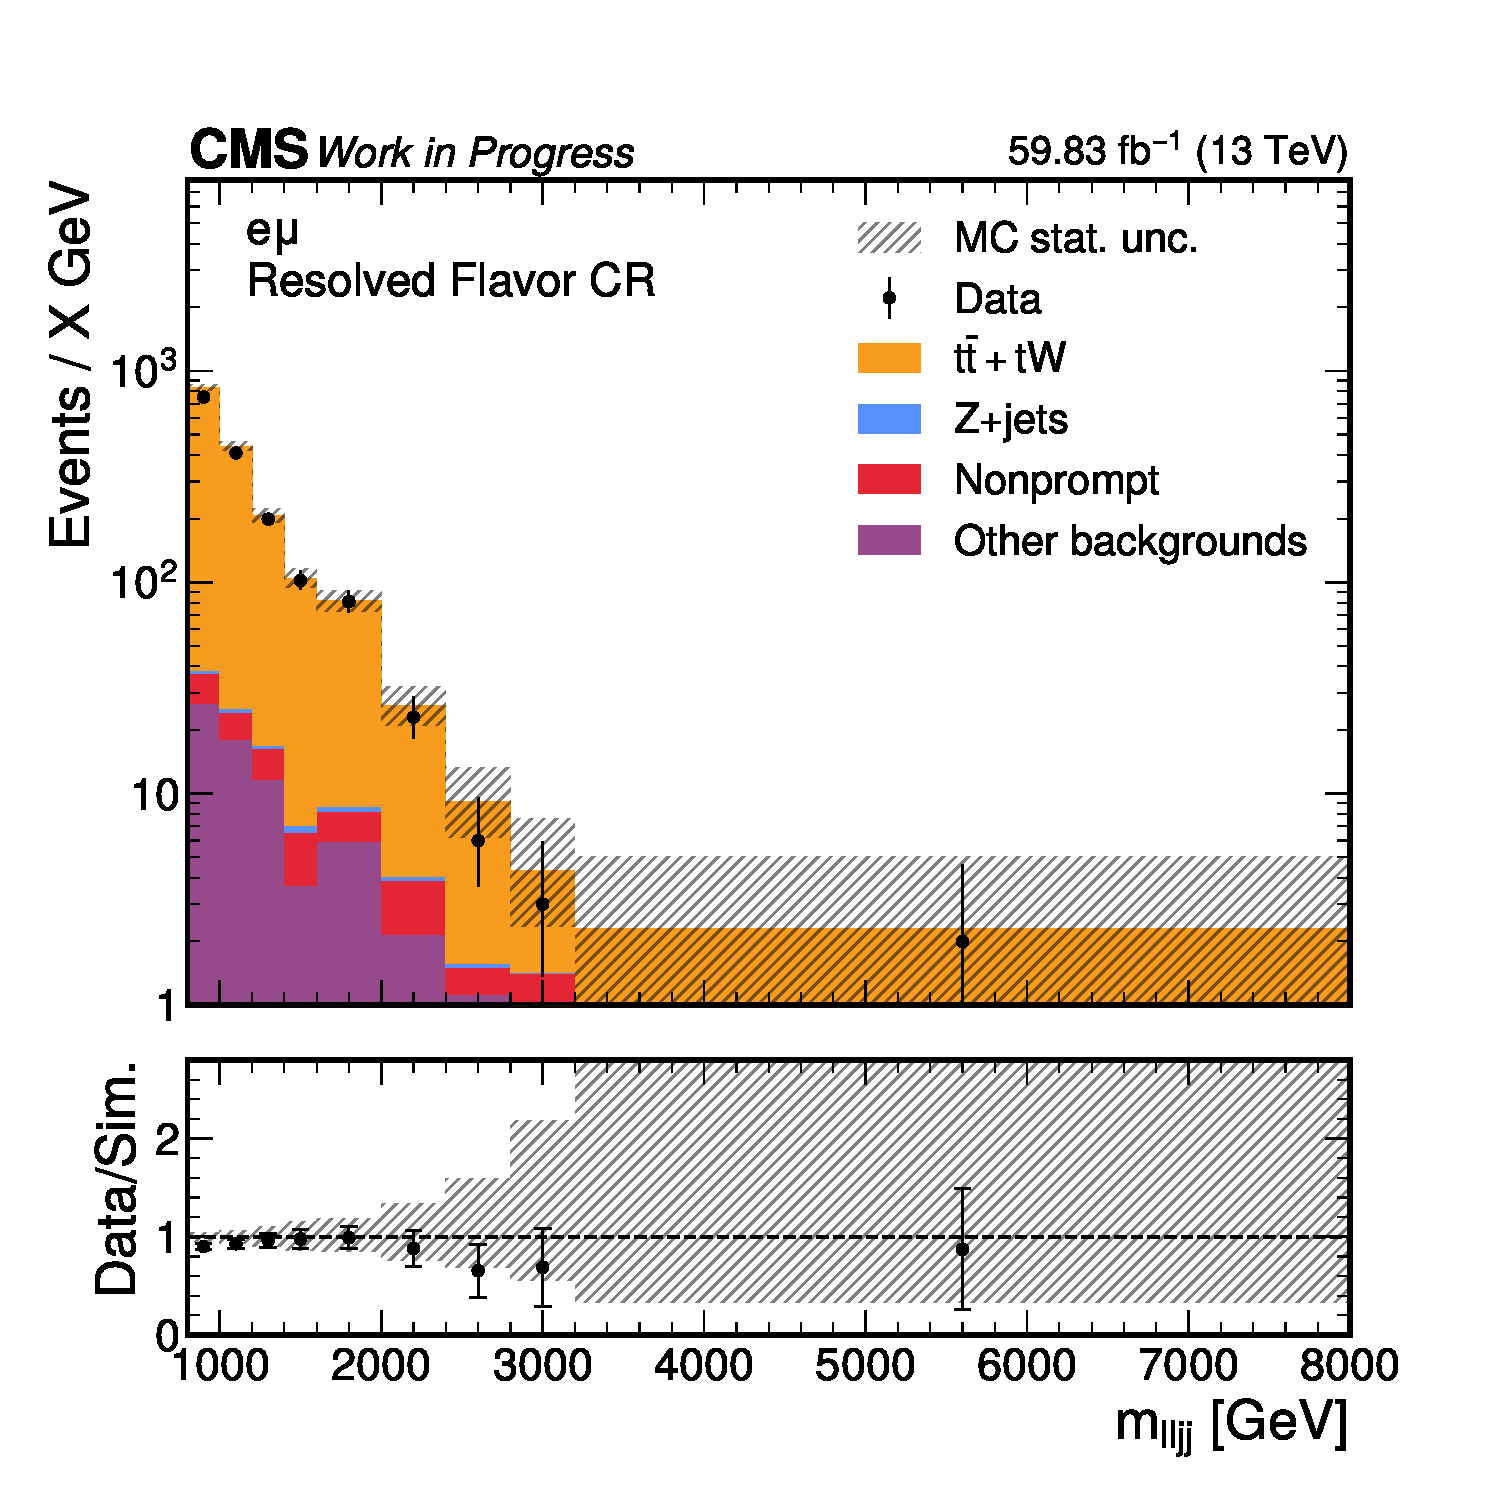
\includegraphics[width=\textwidth]{../figures/plots/mass-fourobject-flavorcr.pdf}
    \end{column}
    \begin{column}{0.50\textwidth}
        \vspace*{-15mm}
        \centering
        \resizebox{\columnwidth}{!}{%
        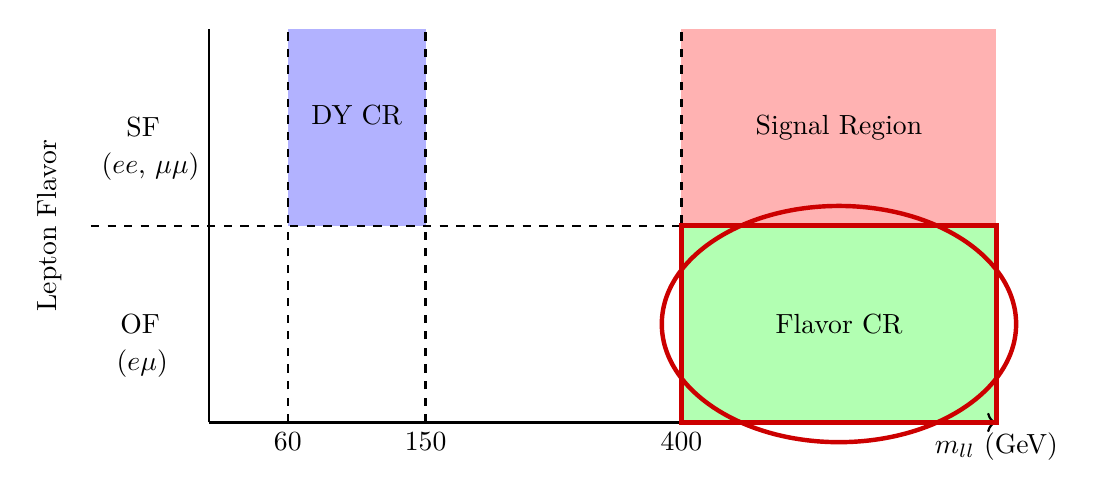
\begin{tikzpicture}[scale=5]
  
    % Define the division points for the vertical regions
    \def\xzero{0.2}   % New left margin division (empty or used for spacing)
    \def\xone{0.55}   % Right boundary of region 1 (DYCR)
    \def\xtwo{1.2}   % Right boundary of region 2 (CR)/left boundary of region 3 (SB)
    \def\xmax{2}      % Overall width of the box

    % -- Fill each grid cell with distinct colors --
    % Column 1: between xzero and xone
    \fill [blue!30!white]    (\xzero,0.5) rectangle (\xone,1);   % Top cell
    \fill [white]    (\xzero,0) rectangle (\xone,0.5);      % Bottom cell

    % Column 2: between xone and xtwo
    \fill [white]   (\xone,0.5) rectangle (\xtwo,1);       % Top cell
    \fill [white]   (\xone,0) rectangle (\xtwo,0.5);         % Bottom cell

    % Column 3: between xtwo and xmax
    \fill [red!30!white]  (\xtwo,0.5) rectangle (\xmax,1);         % Top cell
    \fill [green!30!white]  (\xtwo,0) rectangle (\xmax,0.5);           % Bottom cell
      
    % -- Draw dashed vertical division lines --
    \draw[dashed,thick] (\xzero,0) -- (\xzero,1);  % New left margin boundary
    \draw[dashed,thick] (\xone,0) -- (\xone,1);
    \draw[dashed,thick] (\xtwo,0) -- (\xtwo,1);
    
    % -- Draw a horizontal dashed line (dividing the rows) --
    \draw[dashed,thick] (-0.3,0.5) -- (\xmax,0.5);
    
    % -- Label the y-axis regions (lepton charges) --
    \draw
      (-0.1,0.75) node[anchor=east] {SF}
      (0,0.65) node[anchor=east] {($ee$, $\mu\mu$)}
      (-0.1,0.25) node[anchor=east] {OF}
      (-0.08,0.15) node[anchor=east] {($e\mu$)};
    
    % -- Label the x-axis tick marks (using the original vertical lines) --
    \draw
      (\xzero,0) node[anchor=north] {60}
      (\xone,0) node[anchor=north] {150}
      (\xtwo,0) node[anchor=north] {400};
    
    % -- Axis description on the left --
    \draw
      (-0.35,0.5) node[rotate=90,anchor=south] {Lepton Flavor};
    
    % -- Draw the x-axis as an arrow along the bottom edge --
    \draw[->, thick] (0,0) -- (\xmax,0) node[anchor=north] {$m_{ll}$ (GeV)};
    
    % -- Optionally draw the y-axis line --
    \draw[thick] (0,0) -- (0,1);

    % -- Add internal region labels --
    % Place the label for the DYCR region at the center of the first (red) column:
    \draw ({(\xzero+\xone)/2},0.78) node {DY CR};
    % Place the label for the CR region in the center of the second (blue) column (here using the bottom half for example):
    \draw ({\xtwo+(\xmax-\xtwo)/2},0.25) node[align=center] {Flavor CR};
    % Place the label for the SB region in the center of the third (green) column (using the top half):
    \draw ({\xtwo+(\xmax-\xtwo)/2},0.75) node[align=center] {Signal Region};

      % 1) Outline
    \draw[ultra thick, red!80!black]
      (\xtwo,0.0) rectangle (\xmax,0.5);

    % 2) Or draw a circle
    \draw[ultra thick, red!80!black]
    ({(\xtwo+\xmax)/2},0.25) 
    ellipse [x radius=0.45, y radius=0.30];

\end{tikzpicture}%
        }
      \vspace{1ex} 
      \begin{block}{$t\bar{t}$ Modeling}
        Simulation of $t\bar{t}$ shows good agreement with data in the $e\mu$ sideband.
      \end{block}
    \end{column}
  \end{columns}
\end{frame}

\note[itemize]{
  \item So now moving down the y-axis to our flavor control region, which again has the high 
    dilepton mass but opposite flavor leptons, we can check the modeling of the $t\bar{t}$ 
    background. 
  \item Here, we have the different backgrounds stacked on top of each other. This bottom plot 
    is a ratio directly comparing the total simulation to data.
  \item And overall it agrees pretty well, especially at the lower four object masses, where 
    we have a decent amount of statistics.
  \item And since the only thing that differs between this control region and the signal region 
    is the flavor of one of the leptons, it stands to reason that we can be pretty confident 
    about the $t\bar{t}$ background modeling in our signal region too.
  \item So now I am going to move us up here to the Drell-Yan Control Region so we can look at 
    the Drell-Yan modeling, and this is where things get a little more interesting.
}

\begin{frame}{Drell-Yan Control Region}
  \begin{block}{Mixed Results}
    DY modeling in the DY CR is mixed - better with leptonic variables and worse with hadronic variables.
  \end{block}
  \vfill
  \begin{columns}
    \begin{column}{0.35\textwidth}
      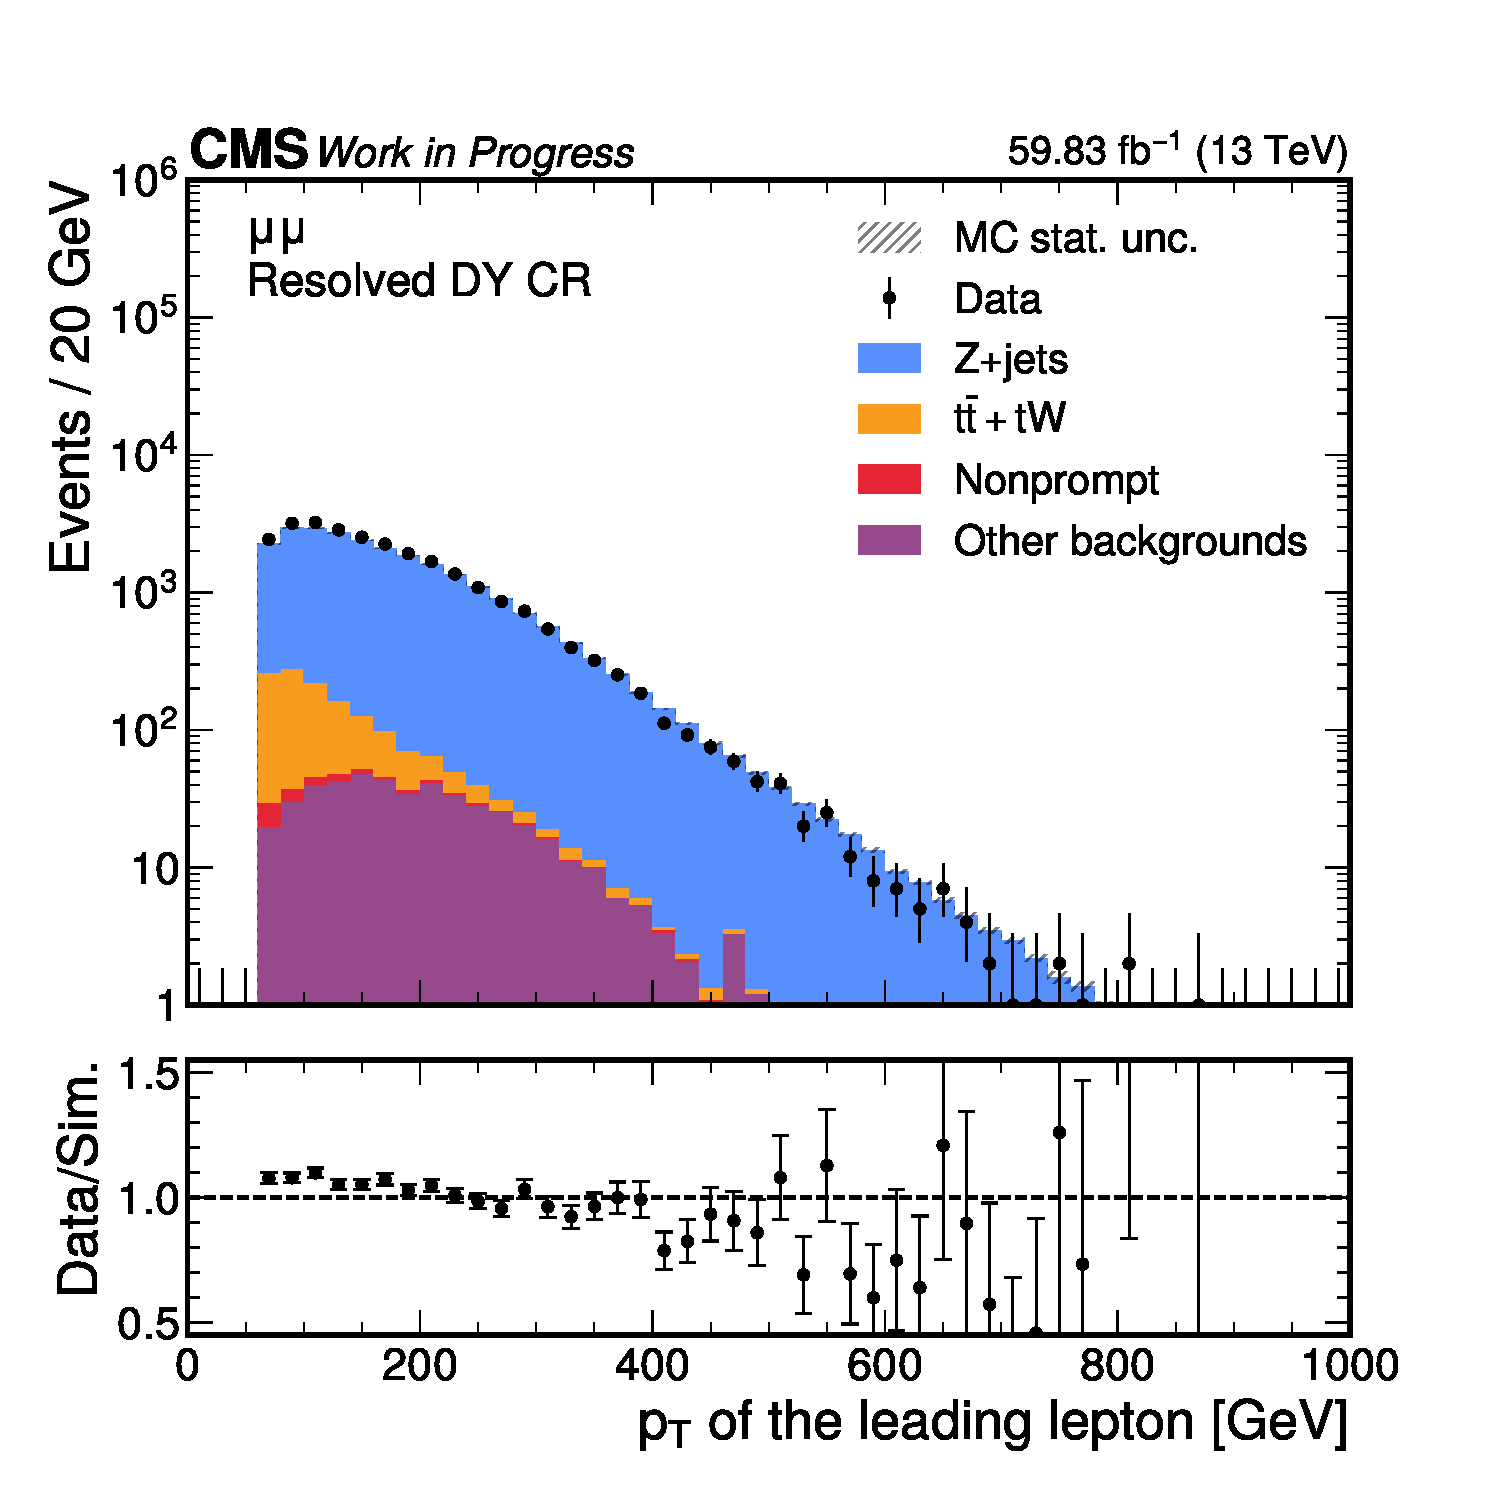
\includegraphics[width=\textwidth]{%
        ../figures/plots/pt-leadlep-dycr-mumu.pdf}
    \end{column}
    \begin{column}{0.35\textwidth}
      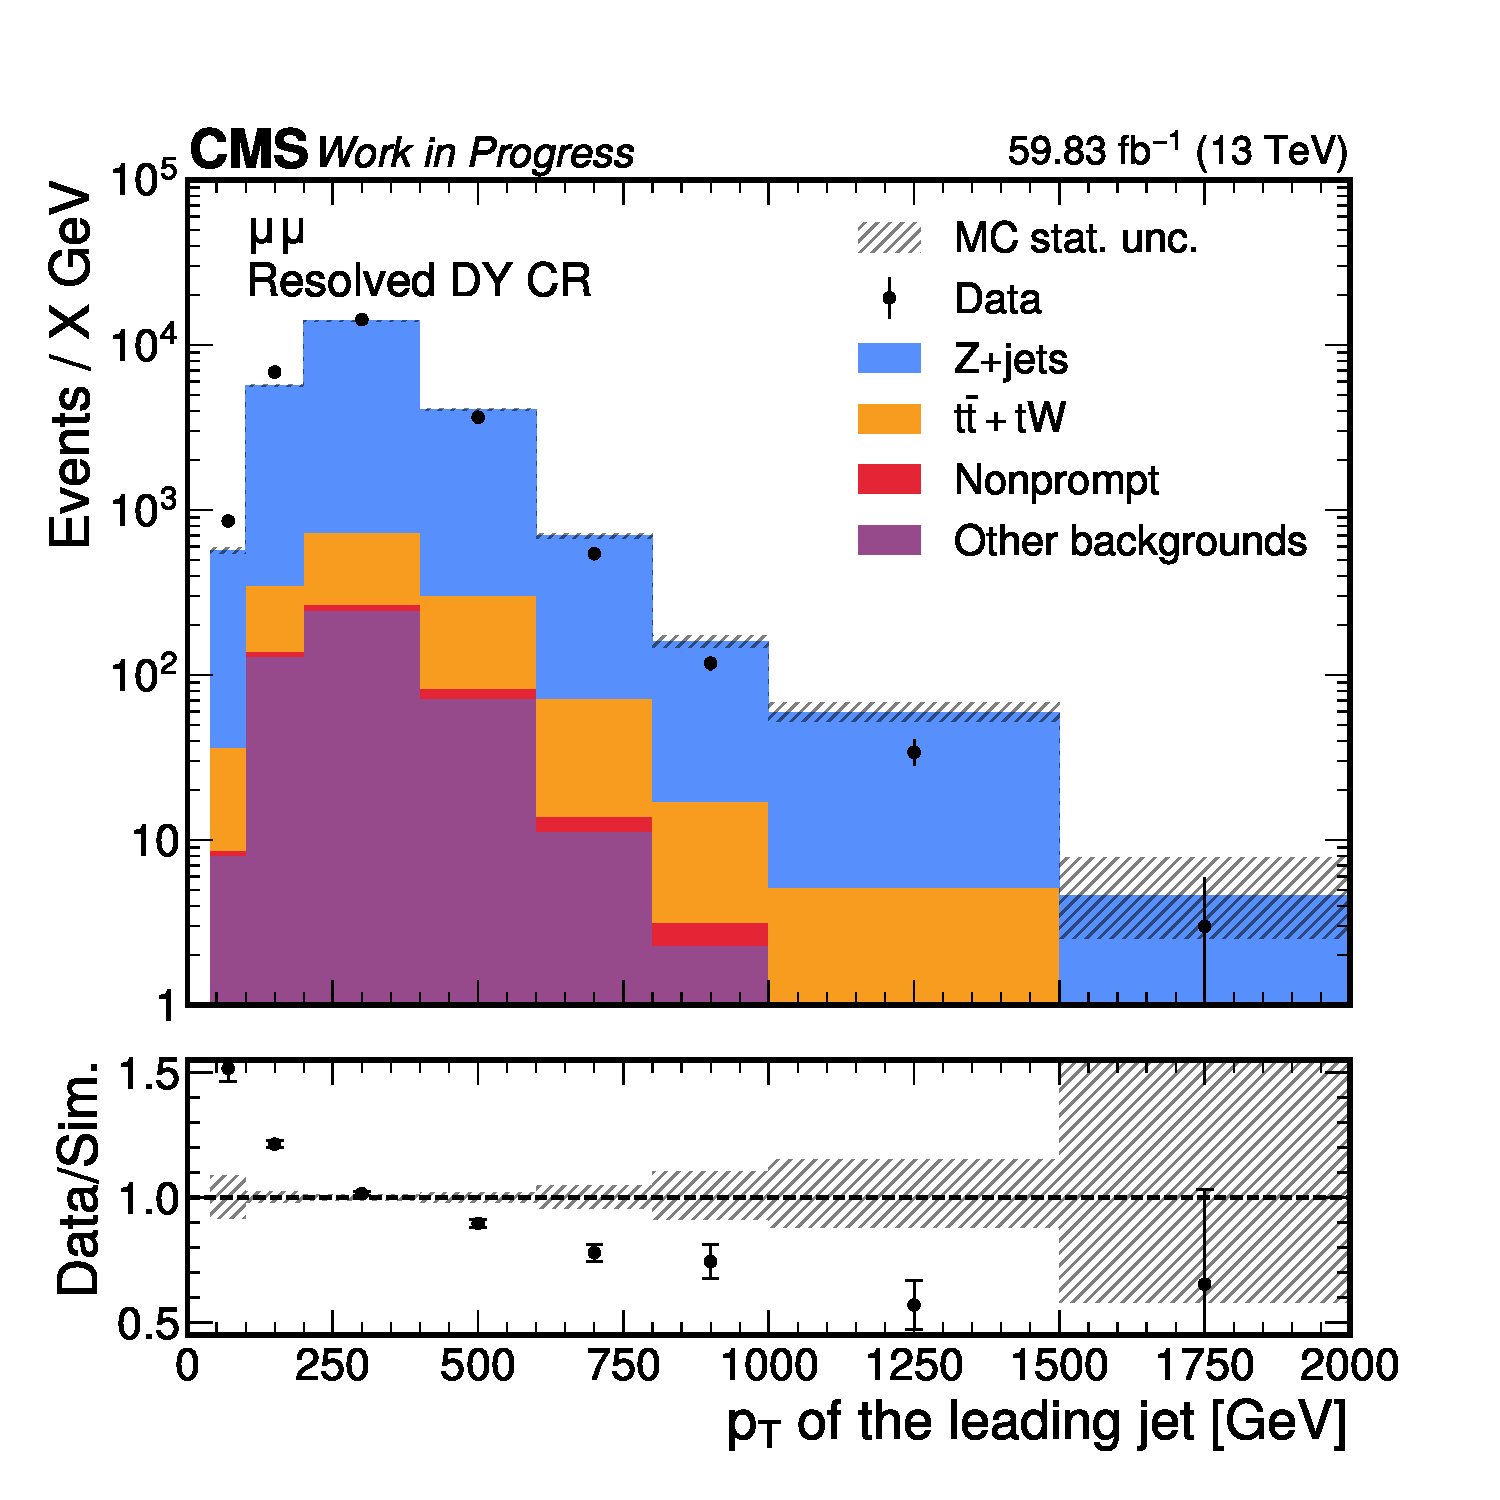
\includegraphics[width=\textwidth]{%
        ../figures/plots/pt-leadjet-dycr-mumu.pdf}
    \end{column}
    \begin{column}{0.3\textwidth}
 %     \vspace*{-15mm}
      \centering
      \resizebox{\columnwidth}{!}{%
      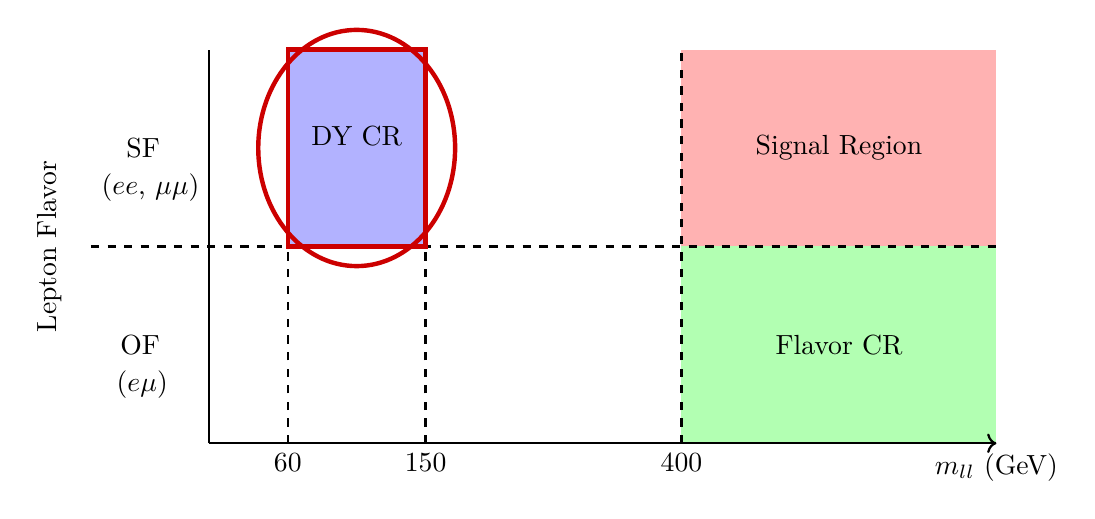
\begin{tikzpicture}[scale=5]
  
    % Define the division points for the vertical regions
    \def\xzero{0.2}   % New left margin division (empty or used for spacing)
    \def\xone{0.55}   % Right boundary of region 1 (DYCR)
    \def\xtwo{1.2}   % Right boundary of region 2 (CR)/left boundary of region 3 (SB)
    \def\xmax{2}      % Overall width of the box

    % -- Fill each grid cell with distinct colors --
    % Column 1: between xzero and xone
    \fill [blue!30!white]    (\xzero,0.5) rectangle (\xone,1);   % Top cell
    \fill [white]    (\xzero,0) rectangle (\xone,0.5);      % Bottom cell

    % Column 2: between xone and xtwo
    \fill [white]   (\xone,0.5) rectangle (\xtwo,1);       % Top cell
    \fill [white]   (\xone,0) rectangle (\xtwo,0.5);         % Bottom cell

    % Column 3: between xtwo and xmax
    \fill [red!30!white]  (\xtwo,0.5) rectangle (\xmax,1);         % Top cell
    \fill [green!30!white]  (\xtwo,0) rectangle (\xmax,0.5);           % Bottom cell
      
    % -- Draw dashed vertical division lines --
    \draw[dashed,thick] (\xzero,0) -- (\xzero,1);  % New left margin boundary
    \draw[dashed,thick] (\xone,0) -- (\xone,1);
    \draw[dashed,thick] (\xtwo,0) -- (\xtwo,1);
    
    % -- Draw a horizontal dashed line (dividing the rows) --
    \draw[dashed,thick] (-0.3,0.5) -- (\xmax,0.5);
    
    % -- Label the y-axis regions (lepton charges) --
    \draw
      (-0.1,0.75) node[anchor=east] {SF}
      (0,0.65) node[anchor=east] {($ee$, $\mu\mu$)}
      (-0.1,0.25) node[anchor=east] {OF}
      (-0.08,0.15) node[anchor=east] {($e\mu$)};
    
    % -- Label the x-axis tick marks (using the original vertical lines) --
    \draw
      (\xzero,0) node[anchor=north] {60}
      (\xone,0) node[anchor=north] {150}
      (\xtwo,0) node[anchor=north] {400};
    
    % -- Axis description on the left --
    \draw
      (-0.35,0.5) node[rotate=90,anchor=south] {Lepton Flavor};
    
    % -- Draw the x-axis as an arrow along the bottom edge --
    \draw[->, thick] (0,0) -- (\xmax,0) node[anchor=north] {$m_{ll}$ (GeV)};
    
    % -- Optionally draw the y-axis line --
    \draw[thick] (0,0) -- (0,1);

    % -- Add internal region labels --
    % Place the label for the DYCR region at the center of the first (red) column:
    \draw ({(\xzero+\xone)/2},0.78) node {DY CR};
    % Place the label for the CR region in the center of the second (blue) column (here using the bottom half for example):
    \draw ({\xtwo+(\xmax-\xtwo)/2},0.25) node[align=center] {Flavor CR};
    % Place the label for the SB region in the center of the third (green) column (using the top half):
    \draw ({\xtwo+(\xmax-\xtwo)/2},0.75) node[align=center] {Signal Region};

      % 1) Outline
    \draw[ultra thick, red!80!black]
      (\xzero,0.5) rectangle (\xone,1.0);

    % 2) Or draw a circle
    \draw[ultra thick, red!80!black]
    ({(\xzero+\xone)/2},0.75) 
    ellipse [x radius=0.25, y radius=0.30];

\end{tikzpicture}%
      }
    \end{column}
  \end{columns}
\end{frame}

\note[itemize]{
  \item When we first look at the Drell-Yan Control Region, we noticed that the electroweak 
    variables are in reasonable agreement, but the hadronic variables are mismodelled.
  \item For example, this plot on the right shows the transverse momentum of the leading jet.
   And you can see in the ratio plot that there is a disagreement between simulation and data 
   across the entire spectrum. 
  \item If you compare that with the transverse momentum of the leading lepton, you can see that 
   there is much better agreement with data.
  \item The cause of the hadronic mismodelling is unknown. We think that in part it may be due 
    to the fact that our Drell-Yan event generator is limited to leading order, and so this could 
    be an effect of neglecting loop corrections, and the additional factors of the strong coupling 
    constant and things like that.
  \item But not knowing exactly what is wrong with the simulations makes it very to fix.
}

\subsection{Correcting the Background}

\begin{frame}{DY MC Reweighting}
  \begin{columns}
    \begin{column}{0.50\textwidth}
      \centering
      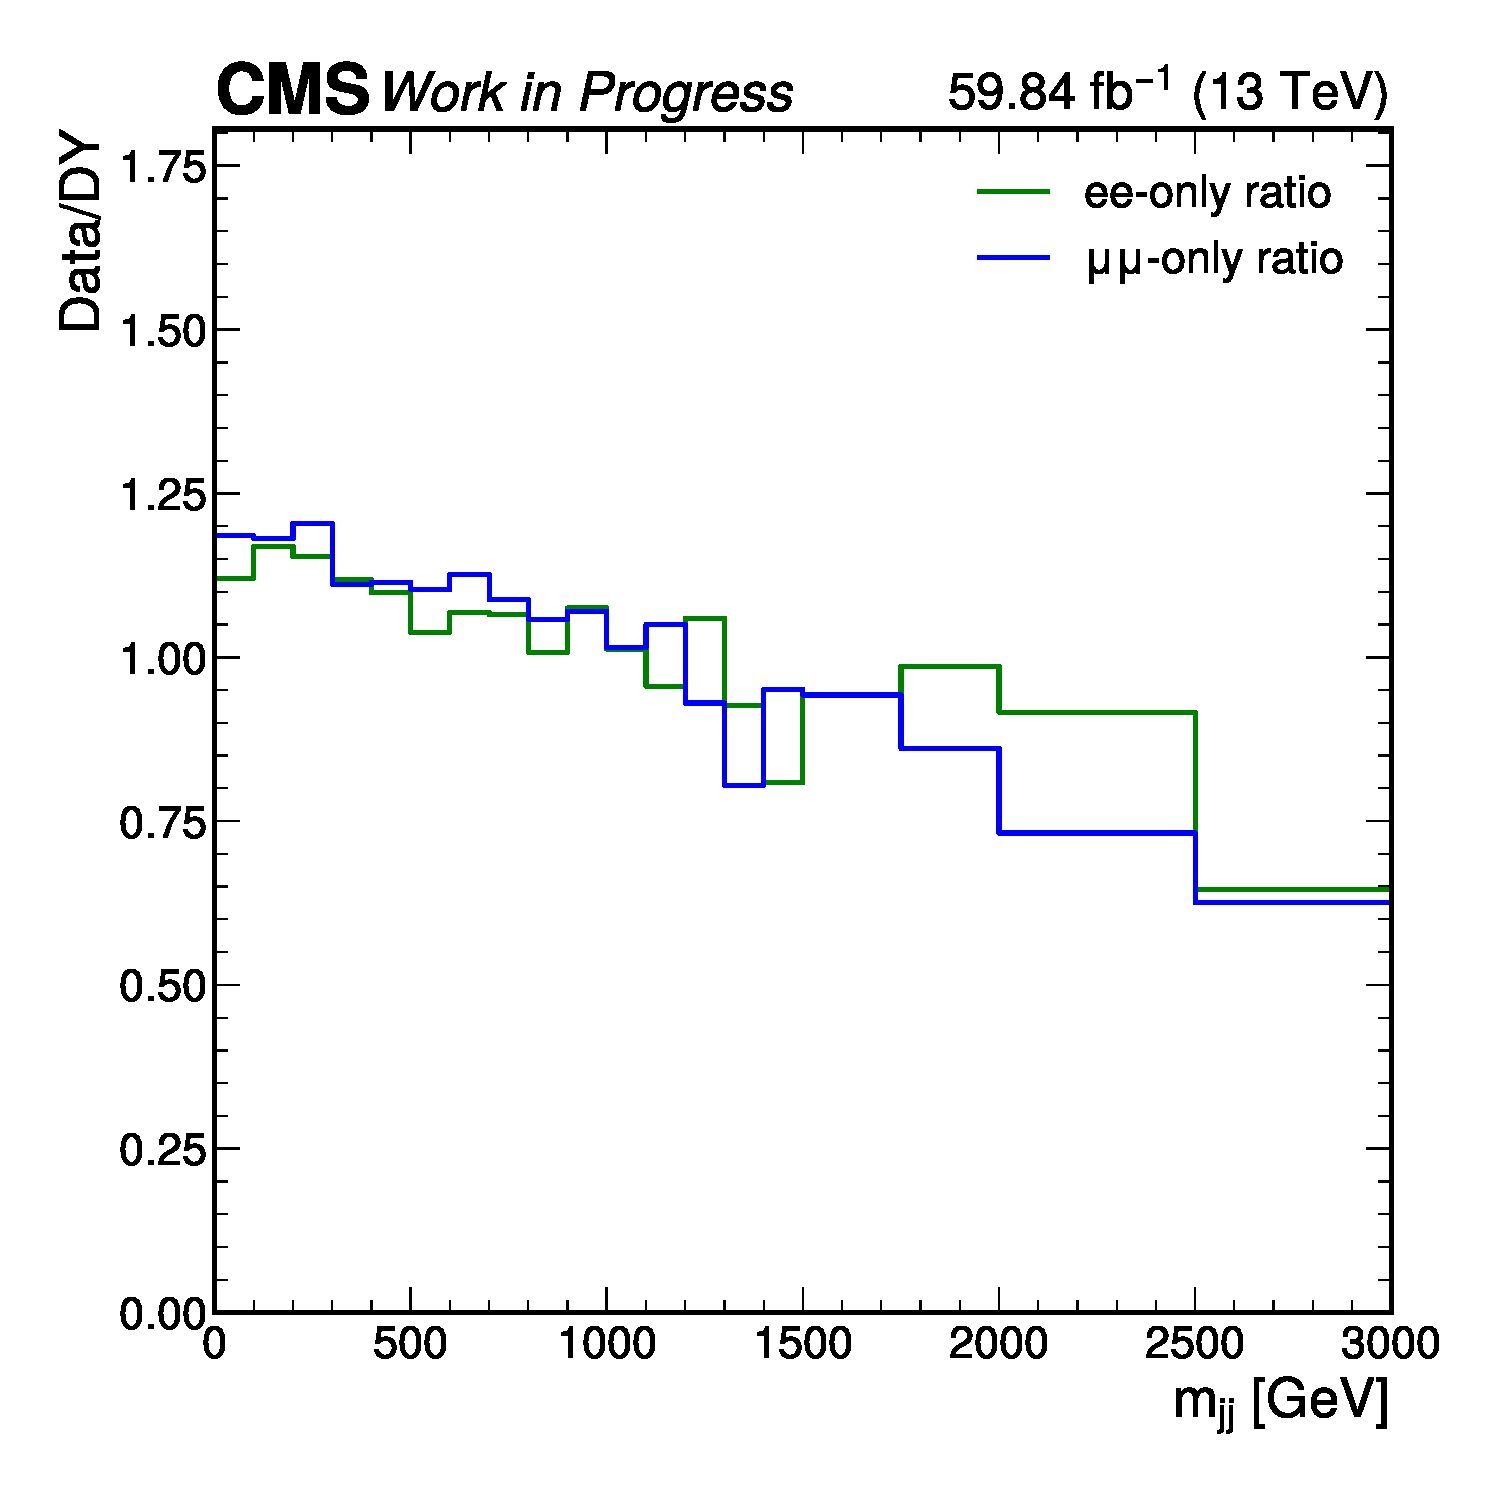
\includegraphics[width=\textwidth]{../figures/plots/mass_sf_ratio.pdf}
    \end{column}
    \begin{column}{0.50\textwidth}
        \centering
        \resizebox{0.55\columnwidth}{!}{%
        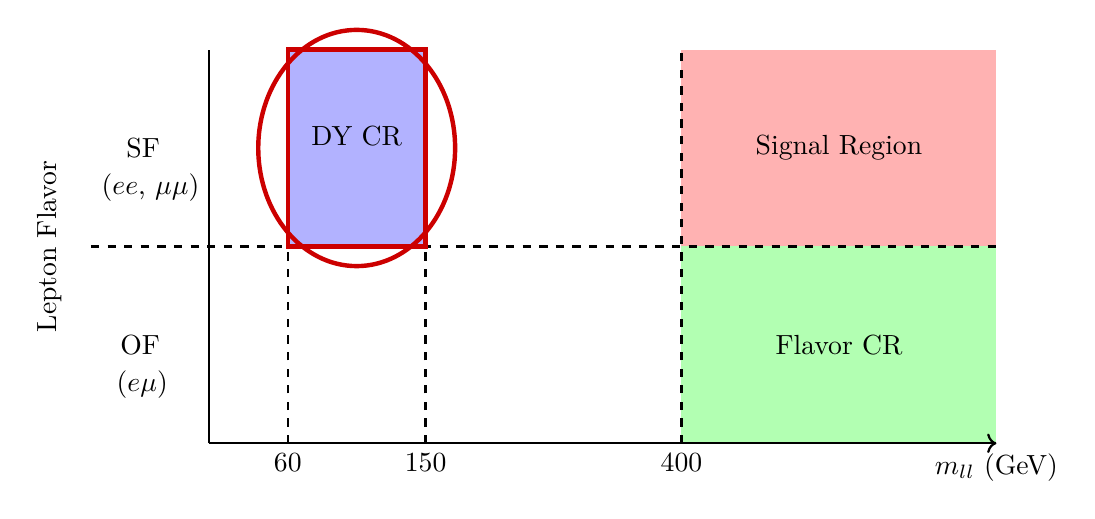
\begin{tikzpicture}[scale=5]
  
    % Define the division points for the vertical regions
    \def\xzero{0.2}   % New left margin division (empty or used for spacing)
    \def\xone{0.55}   % Right boundary of region 1 (DYCR)
    \def\xtwo{1.2}   % Right boundary of region 2 (CR)/left boundary of region 3 (SB)
    \def\xmax{2}      % Overall width of the box

    % -- Fill each grid cell with distinct colors --
    % Column 1: between xzero and xone
    \fill [blue!30!white]    (\xzero,0.5) rectangle (\xone,1);   % Top cell
    \fill [white]    (\xzero,0) rectangle (\xone,0.5);      % Bottom cell

    % Column 2: between xone and xtwo
    \fill [white]   (\xone,0.5) rectangle (\xtwo,1);       % Top cell
    \fill [white]   (\xone,0) rectangle (\xtwo,0.5);         % Bottom cell

    % Column 3: between xtwo and xmax
    \fill [red!30!white]  (\xtwo,0.5) rectangle (\xmax,1);         % Top cell
    \fill [green!30!white]  (\xtwo,0) rectangle (\xmax,0.5);           % Bottom cell
      
    % -- Draw dashed vertical division lines --
    \draw[dashed,thick] (\xzero,0) -- (\xzero,1);  % New left margin boundary
    \draw[dashed,thick] (\xone,0) -- (\xone,1);
    \draw[dashed,thick] (\xtwo,0) -- (\xtwo,1);
    
    % -- Draw a horizontal dashed line (dividing the rows) --
    \draw[dashed,thick] (-0.3,0.5) -- (\xmax,0.5);
    
    % -- Label the y-axis regions (lepton charges) --
    \draw
      (-0.1,0.75) node[anchor=east] {SF}
      (0,0.65) node[anchor=east] {($ee$, $\mu\mu$)}
      (-0.1,0.25) node[anchor=east] {OF}
      (-0.08,0.15) node[anchor=east] {($e\mu$)};
    
    % -- Label the x-axis tick marks (using the original vertical lines) --
    \draw
      (\xzero,0) node[anchor=north] {60}
      (\xone,0) node[anchor=north] {150}
      (\xtwo,0) node[anchor=north] {400};
    
    % -- Axis description on the left --
    \draw
      (-0.35,0.5) node[rotate=90,anchor=south] {Lepton Flavor};
    
    % -- Draw the x-axis as an arrow along the bottom edge --
    \draw[->, thick] (0,0) -- (\xmax,0) node[anchor=north] {$m_{ll}$ (GeV)};
    
    % -- Optionally draw the y-axis line --
    \draw[thick] (0,0) -- (0,1);

    % -- Add internal region labels --
    % Place the label for the DYCR region at the center of the first (red) column:
    \draw ({(\xzero+\xone)/2},0.78) node {DY CR};
    % Place the label for the CR region in the center of the second (blue) column (here using the bottom half for example):
    \draw ({\xtwo+(\xmax-\xtwo)/2},0.25) node[align=center] {Flavor CR};
    % Place the label for the SB region in the center of the third (green) column (using the top half):
    \draw ({\xtwo+(\xmax-\xtwo)/2},0.75) node[align=center] {Signal Region};

      % 1) Outline
    \draw[ultra thick, red!80!black]
      (\xzero,0.5) rectangle (\xone,1.0);

    % 2) Or draw a circle
    \draw[ultra thick, red!80!black]
    ({(\xzero+\xone)/2},0.75) 
    ellipse [x radius=0.25, y radius=0.30];

\end{tikzpicture}
        }
        \vfill
      \begin{block}{}
        \begin{itemize}
          \item \boldcol{UMNMaroon}{Derive reweighting factors from the dijet mass $m_{jj}$.}
          \begin{itemize}
            \item Scale the DY MC in each bin to agree with data. 
          \end{itemize}
          \item Apply these scale factors to all DY MC.
        \end{itemize}
        
      \end{block}
    \end{column}
  \end{columns}
\end{frame}

\note[itemize]{
  \item A technique that is widely used in collider-based physics experiments is to derive and apply 
    a reweighting function based a kinematic variable that encapsulates the mismodelling. In this case, 
    we chose to derive the reweighting function based on the dijet mass spectrum.
  \item The reweighting function is a simple bin-by-bin correction. This plot on the left shows the 
    bin-by-bin values we are applying, and each factor is applied as weights to our Monte Carlo Drell-yan
    background.
  \item So just as an example, in this first bin the blue line for muons is at about 1.2, so if we have a Drell-Yan event
   with a weight of 1, that weight becomes 1.2. 
  \item This scales the Monte Carlo to agree with data in that bin, so that if we were to compare Data and Monte Carlo across
   the entire dijet mass spectrum after reweighting, there would be good agreement between them.
  \item And then finally, these re-weighting factors are then propagated to all of our kinematic variables 
  across all analysis regions.
}

\begin{frame}{DY CR Reweighted}
  \begin{columns}
    \begin{column}{0.69\textwidth}
      \begin{block}{}
        \centering
        The reweighting improves the Drell-Yan modeling in the DY control region.
      \end{block}
    \end{column}
    \begin{column}{0.3\textwidth}
      \centering
      \resizebox{0.9\columnwidth}{!}{%
      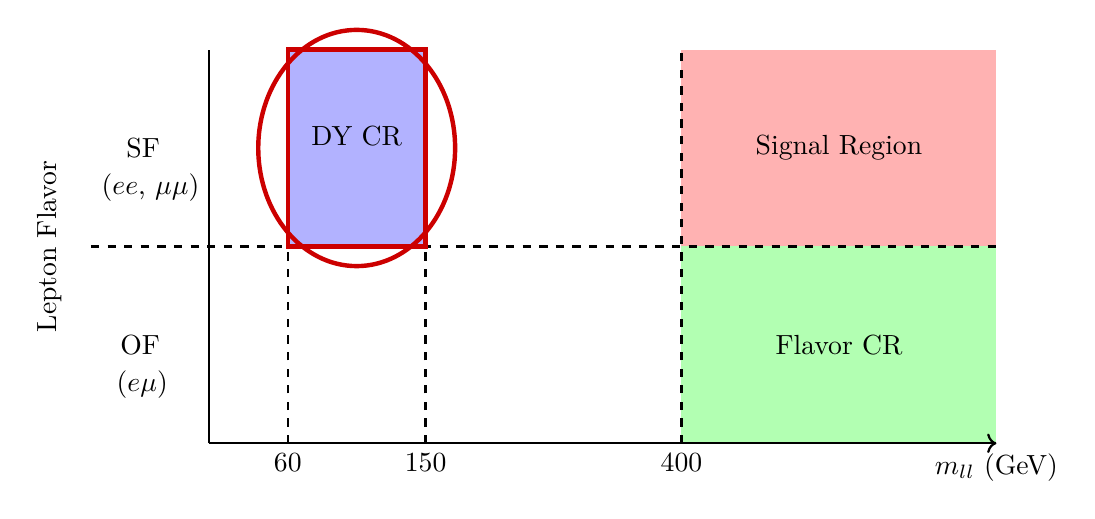
\begin{tikzpicture}[scale=5]
  
    % Define the division points for the vertical regions
    \def\xzero{0.2}   % New left margin division (empty or used for spacing)
    \def\xone{0.55}   % Right boundary of region 1 (DYCR)
    \def\xtwo{1.2}   % Right boundary of region 2 (CR)/left boundary of region 3 (SB)
    \def\xmax{2}      % Overall width of the box

    % -- Fill each grid cell with distinct colors --
    % Column 1: between xzero and xone
    \fill [blue!30!white]    (\xzero,0.5) rectangle (\xone,1);   % Top cell
    \fill [white]    (\xzero,0) rectangle (\xone,0.5);      % Bottom cell

    % Column 2: between xone and xtwo
    \fill [white]   (\xone,0.5) rectangle (\xtwo,1);       % Top cell
    \fill [white]   (\xone,0) rectangle (\xtwo,0.5);         % Bottom cell

    % Column 3: between xtwo and xmax
    \fill [red!30!white]  (\xtwo,0.5) rectangle (\xmax,1);         % Top cell
    \fill [green!30!white]  (\xtwo,0) rectangle (\xmax,0.5);           % Bottom cell
      
    % -- Draw dashed vertical division lines --
    \draw[dashed,thick] (\xzero,0) -- (\xzero,1);  % New left margin boundary
    \draw[dashed,thick] (\xone,0) -- (\xone,1);
    \draw[dashed,thick] (\xtwo,0) -- (\xtwo,1);
    
    % -- Draw a horizontal dashed line (dividing the rows) --
    \draw[dashed,thick] (-0.3,0.5) -- (\xmax,0.5);
    
    % -- Label the y-axis regions (lepton charges) --
    \draw
      (-0.1,0.75) node[anchor=east] {SF}
      (0,0.65) node[anchor=east] {($ee$, $\mu\mu$)}
      (-0.1,0.25) node[anchor=east] {OF}
      (-0.08,0.15) node[anchor=east] {($e\mu$)};
    
    % -- Label the x-axis tick marks (using the original vertical lines) --
    \draw
      (\xzero,0) node[anchor=north] {60}
      (\xone,0) node[anchor=north] {150}
      (\xtwo,0) node[anchor=north] {400};
    
    % -- Axis description on the left --
    \draw
      (-0.35,0.5) node[rotate=90,anchor=south] {Lepton Flavor};
    
    % -- Draw the x-axis as an arrow along the bottom edge --
    \draw[->, thick] (0,0) -- (\xmax,0) node[anchor=north] {$m_{ll}$ (GeV)};
    
    % -- Optionally draw the y-axis line --
    \draw[thick] (0,0) -- (0,1);

    % -- Add internal region labels --
    % Place the label for the DYCR region at the center of the first (red) column:
    \draw ({(\xzero+\xone)/2},0.78) node {DY CR};
    % Place the label for the CR region in the center of the second (blue) column (here using the bottom half for example):
    \draw ({\xtwo+(\xmax-\xtwo)/2},0.25) node[align=center] {Flavor CR};
    % Place the label for the SB region in the center of the third (green) column (using the top half):
    \draw ({\xtwo+(\xmax-\xtwo)/2},0.75) node[align=center] {Signal Region};

      % 1) Outline
    \draw[ultra thick, red!80!black]
      (\xzero,0.5) rectangle (\xone,1.0);

    % 2) Or draw a circle
    \draw[ultra thick, red!80!black]
    ({(\xzero+\xone)/2},0.75) 
    ellipse [x radius=0.25, y radius=0.30];

\end{tikzpicture}
      }
    \end{column}
  \end{columns}
  \begin{columns}
    \begin{column}{0.35\textwidth}
      \begin{figure}
        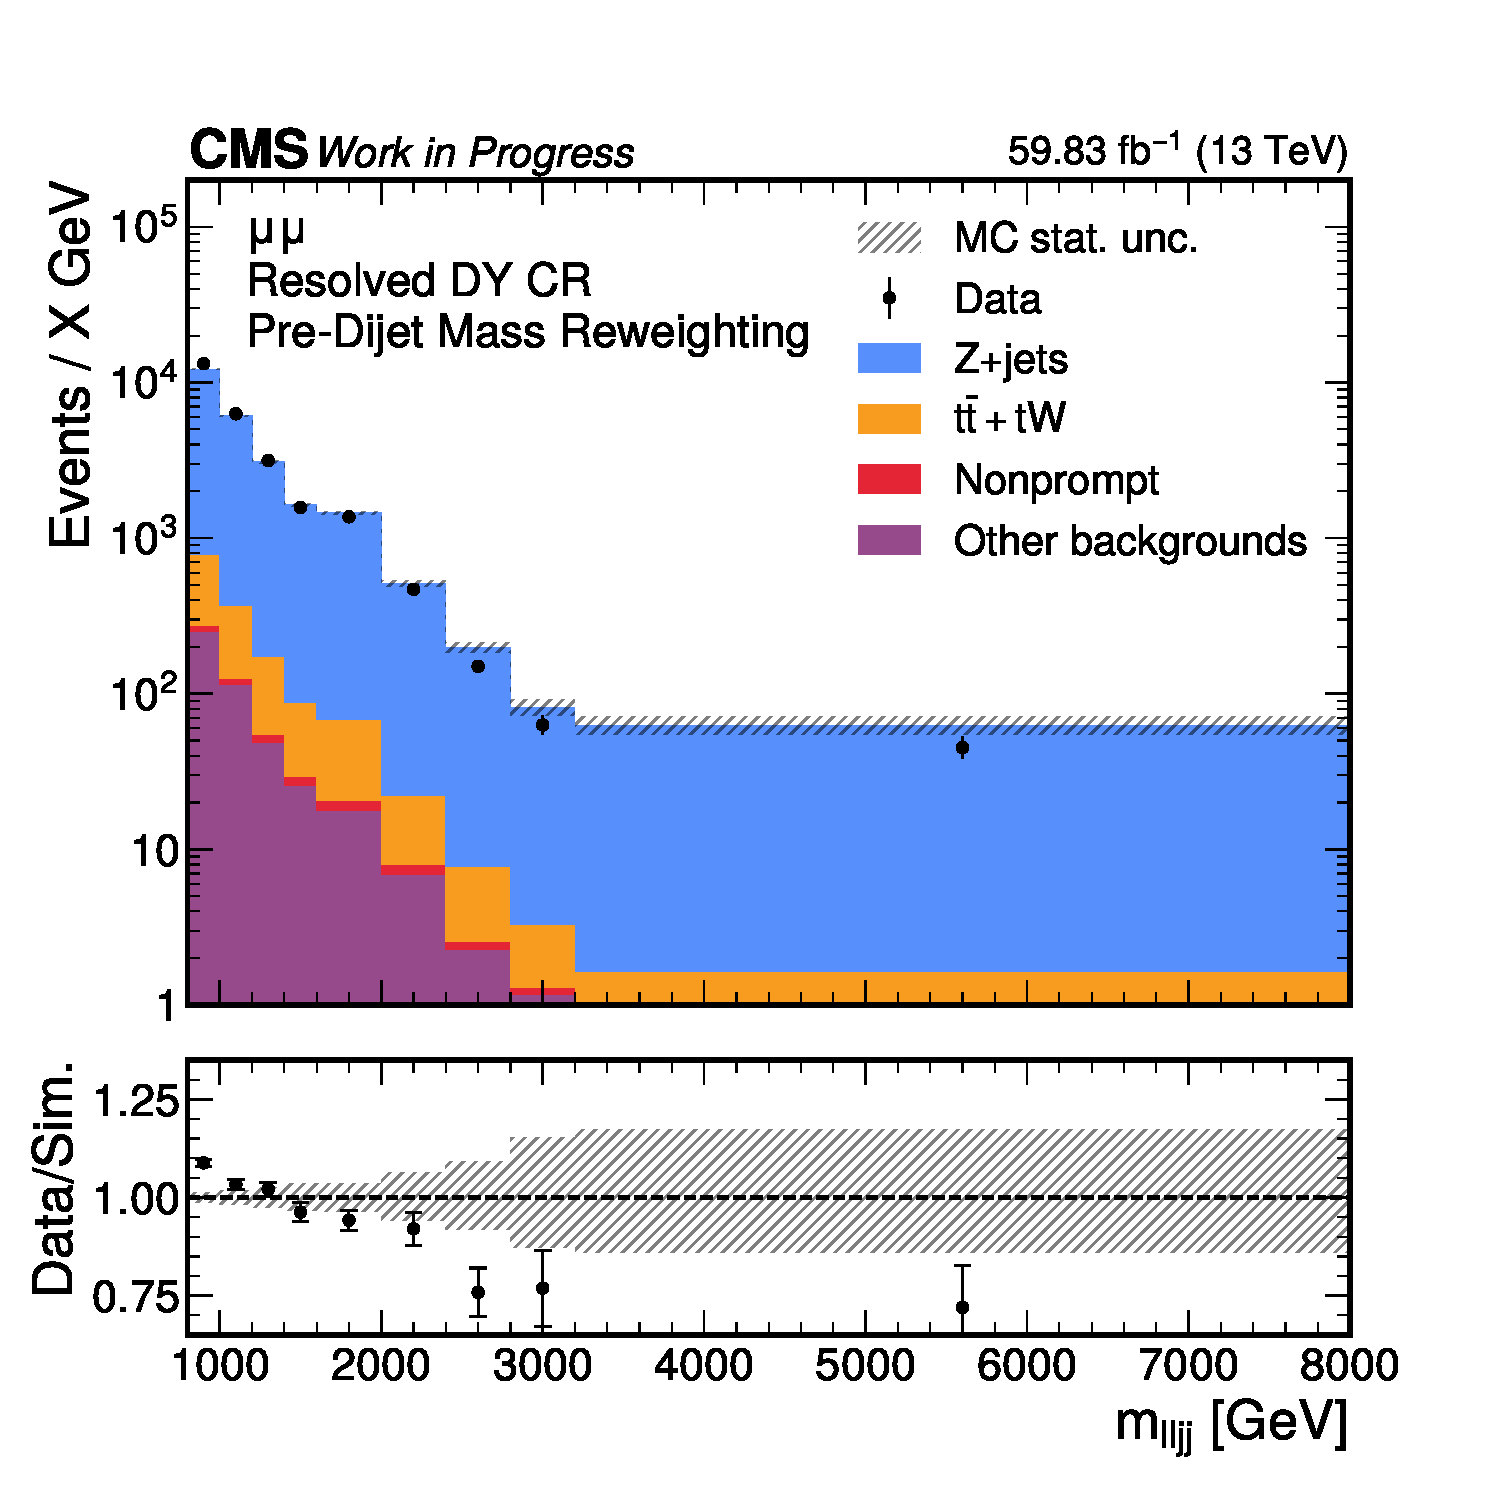
\includegraphics[width=\textwidth]{%
        ../figures/plots/mlljj-dycr-mumu-pre.pdf}
        \caption{pre-ratio}
      \end{figure}
    \end{column}
    \begin{column}{0.35\textwidth}
      \begin{figure}
        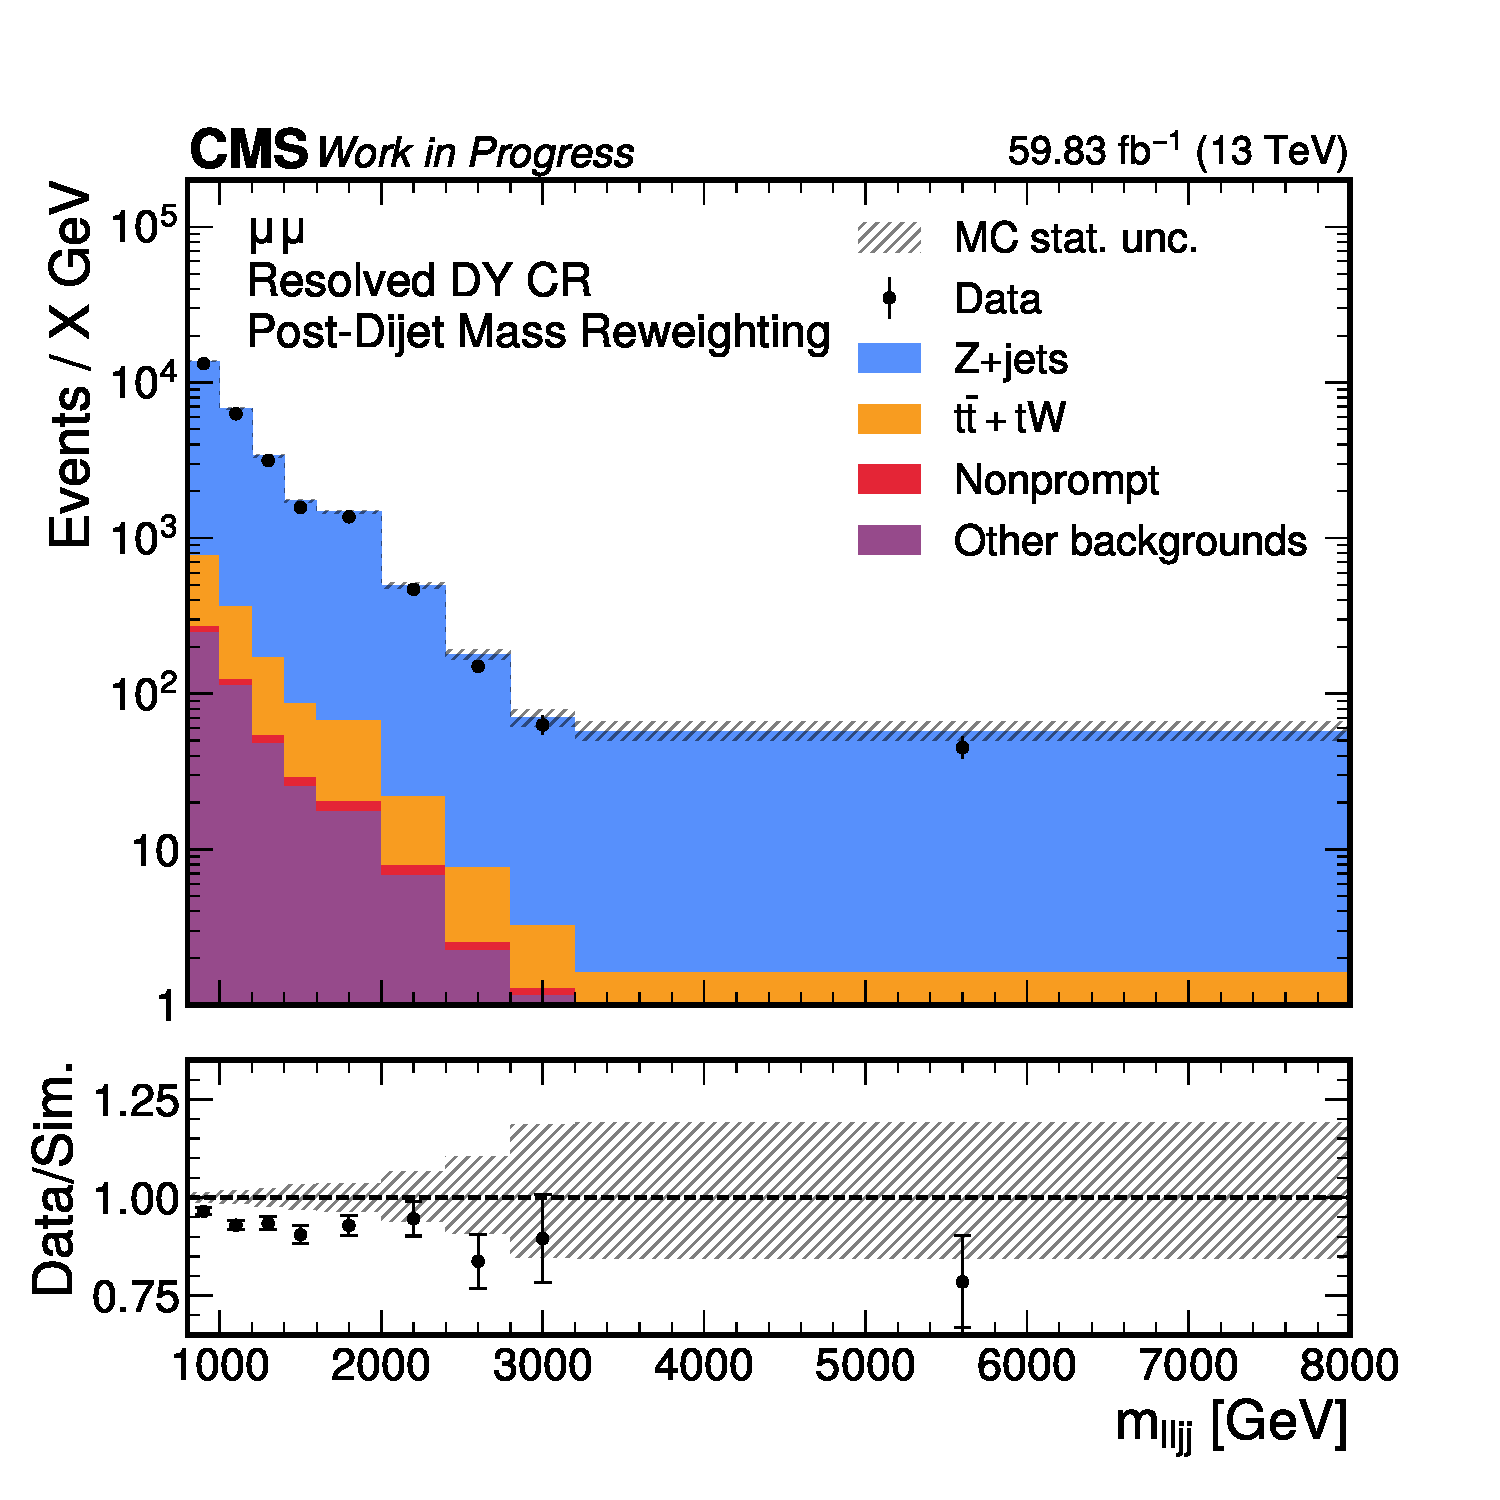
\includegraphics[width=\textwidth]{%
        ../figures/plots/mlljj-dycr-mumu-post.pdf}
        \caption{post-ratio}
      \end{figure}
    \end{column}
    \begin{column}{0.3\textwidth}
      \begin{block}{}
        How does reweighting affect the signal region?
          \begin{itemize}
            \footnotesize
            \item Requires unblinding.
          \end{itemize}
      \end{block}
    \end{column}
  \end{columns}
\end{frame}

\note[itemize]{
  \footnotesize
  \item Here is a plot of our four object invariant mass in the Control Region.
  \item On the left is the four-object mass in the drell-yan control region without any reweighting applied. 
    Looking at this bottom ratio plot, we see that there is a discrepancy between the simulation without corrections and data.  
  \item And the discrepancy has a pretty clear slope to it, where at low mass we are underpredicting the background, and at high
    mass we overpredict it.
  \item The plot on the right is the same plot, except we have applied those dijet mass reweighting factors to the blue 
   Drell-Yan background. 
  \item And you can see that it flattens out the ratio plot, so its pulling up the background in the low mass
   region, and pulling it down a smidge in the high mass region.
  \item There still an overall disagreement, but this can be fixed by applying some overall scale factor, which wouldn't have 
   really helped before the reweighting.
  \item So, the correction works well in the Drell-Yan control region, but the question we really care about is how does this 
    reweighting affect the signal region?
  \item And the answer is that we don't know because that requires unblinding, and I would be in a lot of trouble if I made and 
    showed those plots today. 
}

\section{Looking Forward to Run 3}

\begin{frame}{$m_{\ell \ell}$ optimization}
  \begin{columns}
    \begin{column}{0.50\textwidth}
      \centering
      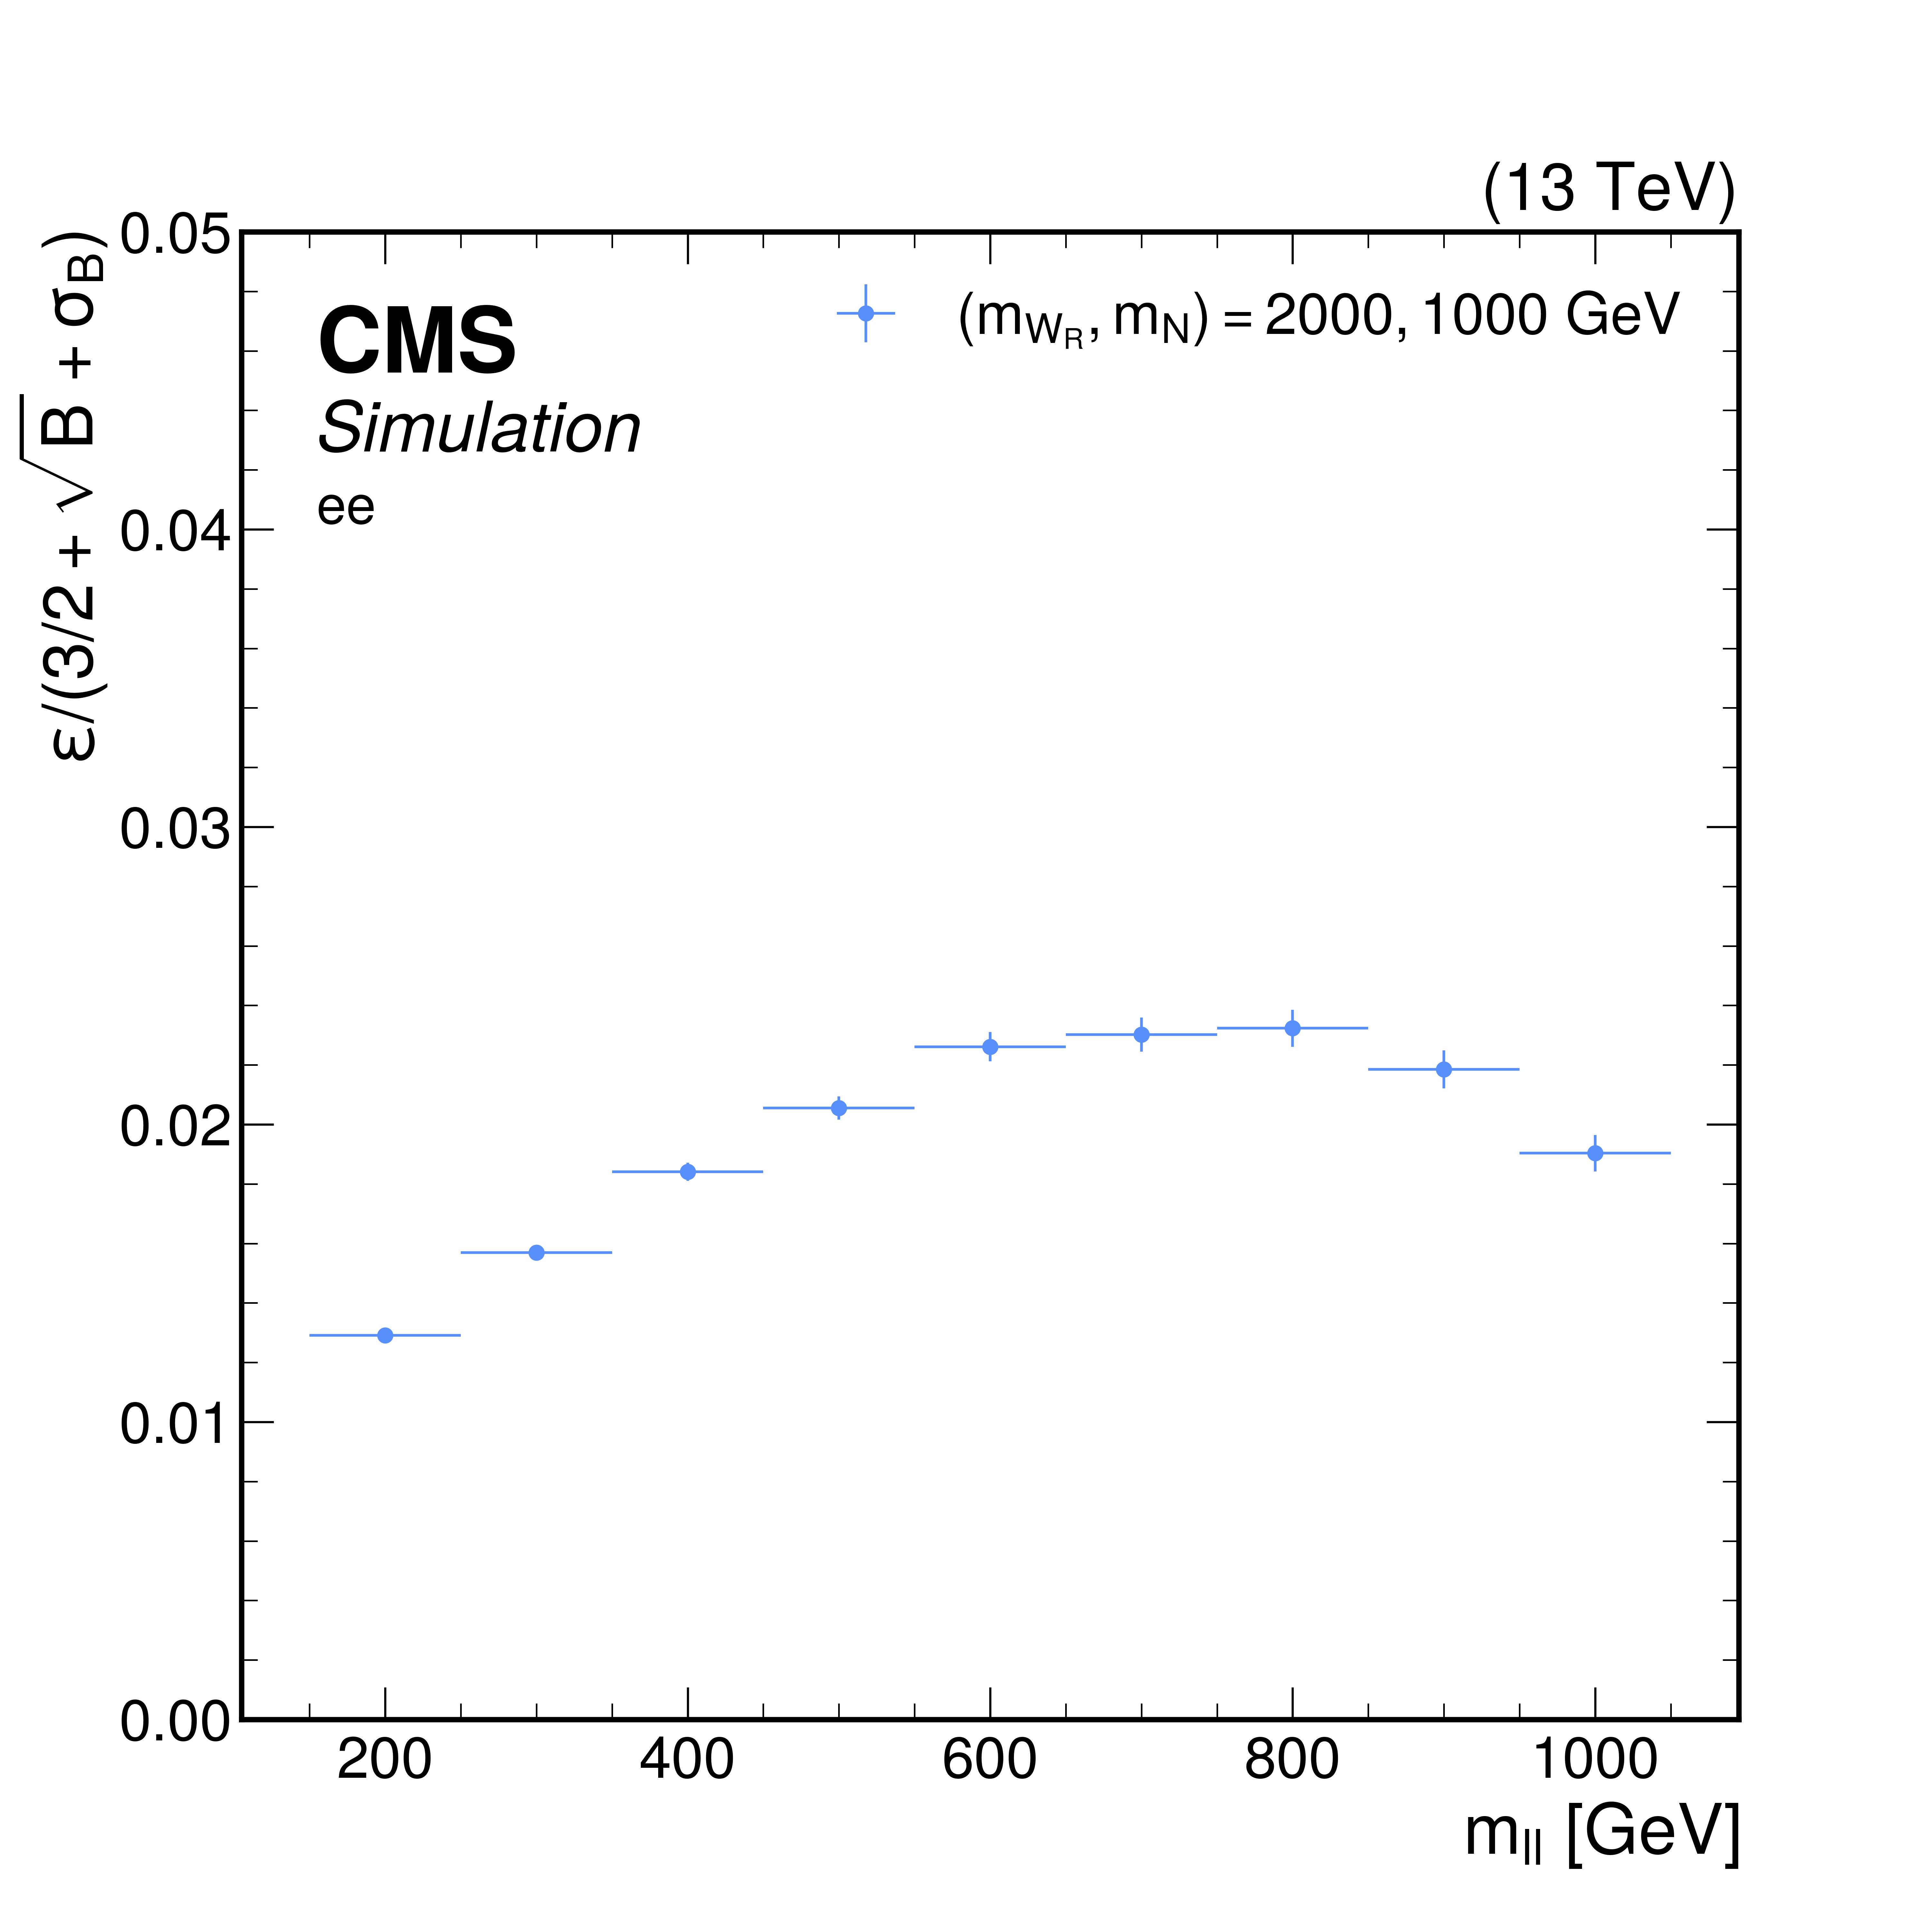
\includegraphics[width=\textwidth]{../figures/plots/mll-optimization.png}
    \end{column}
    \begin{column}{0.50\textwidth}
 %       \vspace*{-5mm}
        \centering
        \resizebox{\columnwidth}{!}{%
        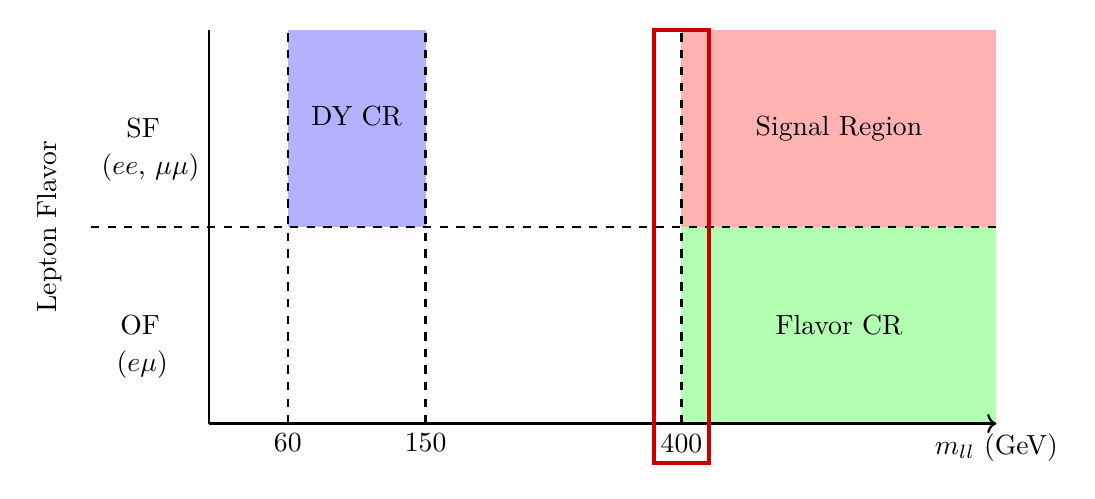
\begin{tikzpicture}[scale=5]
  
    % Define the division points for the vertical regions
    \def\xzero{0.2}   % New left margin division (empty or used for spacing)
    \def\xone{0.55}   % Right boundary of region 1 (DYCR)
    \def\xtwo{1.2}   % Right boundary of region 2 (CR)/left boundary of region 3 (SB)
    \def\xmax{2}      % Overall width of the box

    % -- Fill each grid cell with distinct colors --
    % Column 1: between xzero and xone
    \fill [blue!30!white]    (\xzero,0.5) rectangle (\xone,1);   % Top cell
    \fill [white]    (\xzero,0) rectangle (\xone,0.5);      % Bottom cell

    % Column 2: between xone and xtwo
    \fill [white]   (\xone,0.5) rectangle (\xtwo,1);       % Top cell
    \fill [white]   (\xone,0) rectangle (\xtwo,0.5);         % Bottom cell

    % Column 3: between xtwo and xmax
    \fill [red!30!white]  (\xtwo,0.5) rectangle (\xmax,1);         % Top cell
    \fill [green!30!white]  (\xtwo,0) rectangle (\xmax,0.5);           % Bottom cell
      
    % -- Draw dashed vertical division lines --
    \draw[dashed,thick] (\xzero,0) -- (\xzero,1);  % New left margin boundary
    \draw[dashed,thick] (\xone,0) -- (\xone,1);
    \draw[dashed,thick] (\xtwo,0) -- (\xtwo,1);
    
    % -- Draw a horizontal dashed line (dividing the rows) --
    \draw[dashed,thick] (-0.3,0.5) -- (\xmax,0.5);
    
    % -- Label the y-axis regions (lepton charges) --
    \draw
      (-0.1,0.75) node[anchor=east] {SF}
      (0,0.65) node[anchor=east] {($ee$, $\mu\mu$)}
      (-0.1,0.25) node[anchor=east] {OF}
      (-0.08,0.15) node[anchor=east] {($e\mu$)};
    
    % -- Label the x-axis tick marks (using the original vertical lines) --
    \draw
      (\xzero,0) node[anchor=north] {60}
      (\xone,0) node[anchor=north] {150}
      (\xtwo,0) node[anchor=north] {400};
    
    % -- Axis description on the left --
    \draw
      (-0.35,0.5) node[rotate=90,anchor=south] {Lepton Flavor};
    
    % -- Draw the x-axis as an arrow along the bottom edge --
    \draw[->, thick] (0,0) -- (\xmax,0) node[anchor=north] {$m_{ll}$ (GeV)};
    
    % -- Optionally draw the y-axis line --
    \draw[thick] (0,0) -- (0,1);

    % -- Add internal region labels --
    % Place the label for the DYCR region at the center of the first (red) column:
    \draw ({(\xzero+\xone)/2},0.78) node {DY CR};
    % Place the label for the CR region in the center of the second (blue) column (here using the bottom half for example):
    \draw ({\xtwo+(\xmax-\xtwo)/2},0.25) node[align=center] {Flavor CR};
    % Place the label for the SB region in the center of the third (green) column (using the top half):
    \draw ({\xtwo+(\xmax-\xtwo)/2},0.75) node[align=center] {Signal Region};

      % 1) Outline
   % \draw[ultra thick, red!80!black]
   %   (\xtwo,0.5) rectangle (\xmax,1);

    % 2) Or draw a circle
    \draw[ultra thick, red!80!black]
    (\xtwo-0.07,-0.1) rectangle (\xtwo+0.07,1.00);

\end{tikzpicture}%
        }
 %     \vspace{1ex} 
      \begin{block}{Optimizing the signal region}
        Is $m_{\ell \ell} > 400 \mathrm{~GeV}$ the best cut for the signal region?
      \end{block}
    \end{column}
  \end{columns}
\end{frame}

\note[itemize]{
  \item But something else we've been working on that I can show to wrap things up is this signal region
   optimization study.
  \item So the question this is getting at is, is $m_{ll} > 400$ GeV the best cut for the signal region?
  \item Or, for example, should we loosen the cut, which would amount to sliding this line to the left?
  \item Most commonly this kind of question is answered with an S over root B type of study.
  \item And here on the left we have a similar figure of merit, except we use the signal efficiency instead 
   of the signal yield, and there are some terms in the denominator that prevent the curve from blowing up 
   when the background goes to zero.
  \item And so we can see that our current cut sits on the rising edge of optimal sensitivity and the curve 
   plateus between 600 and 800 GeV.
  \item And so this suggests the 400 GeV cut might be slightly conservative for this signal mass point, but 
    I still need to check what the curves look like for a varity of different WR and signal masses.
}

\section{Conclusion} % \ssection{Conclusion}

\begin{frame}{Conclusion}
  Many improvements and areas of study under development in the $\mathrm{W_R}$ and $\mathrm{N}$ search:

  \begin{columns} % [t] for top alignment of columns
    %――――――――――――――――――――――――――――
    \begin{column}{0.5\textwidth}
      \begin{block}{Looking Forward to Run 3}
        \begin{itemize}
          \item Beginning comparisons for \boldcol{UMNMaroon}{Run 3} Data/MC.
          \item Looking at how \boldcol{UMNMaroon}{adding a third jet} to the final‐state objects affects 
          signal and background yields.
        \end{itemize}
      \end{block}
    \end{column}

    %――――――――――――――――――――――――――――
    \begin{column}{0.5\textwidth}
      \centering
      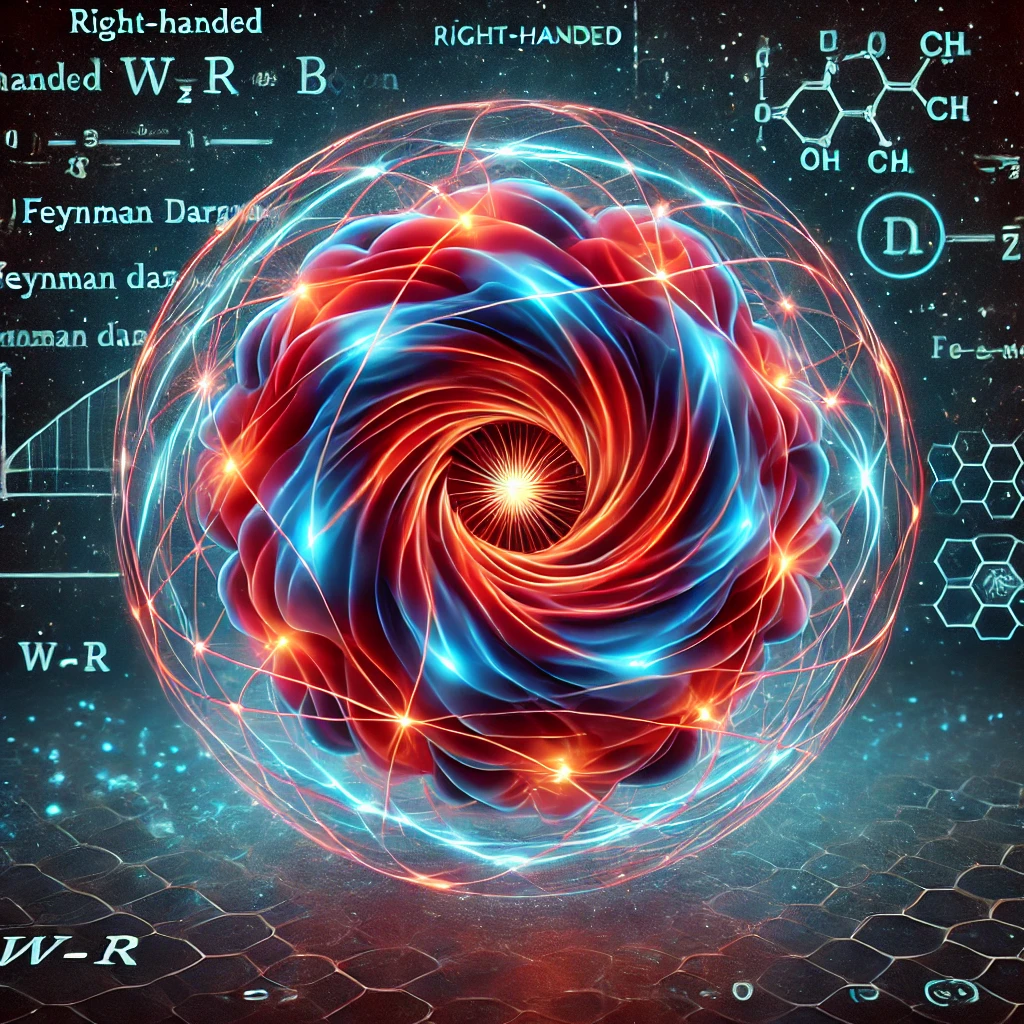
\includegraphics[width=0.75\textwidth]{wr-boson-chatgpt.png}
    \end{column}
  \end{columns}
\end{frame}

\note[itemize]{
  \item OK so in conclusion, there are many improvements and areas of study under development in the 
   right-handed W and heavy neutrino search. 
  \item Namely, we are starting to do preliminary data and Monte Carlo comparisons in our control 
   regions for Run 3.
  \item And we have another graduate student, Sam, who has been looking at how adding a third jet to the 
   final state objects affects signal and background yields. 
  \item So most of the time extra jets in events will be soft, but maybe once in a while a third jet is 
   radiated that carries a substantial fraction of the momentum, and so by not capturing that jet we'd be 
   under-shooting the right-handed W mass. 
  \item And so Sam is looking at seeing if we can distinguish between events where we should be capturing 
    2 vs 3 jets, which might tighten up some of our signal peaks.
  \item And then finally of course on the right here I've included an image what ChatGPT thinks the right-handed W 
  might look like, so we have some idea of what to keep an eye out for.
  \item But with that, does anyone have any questions?
  }

\begin{backup}
  \subsection{Run 2 Results}

  \begin{frame}{Signal Region}
    \begin{columns}
      \begin{column}{0.50\textwidth}
        \centering
        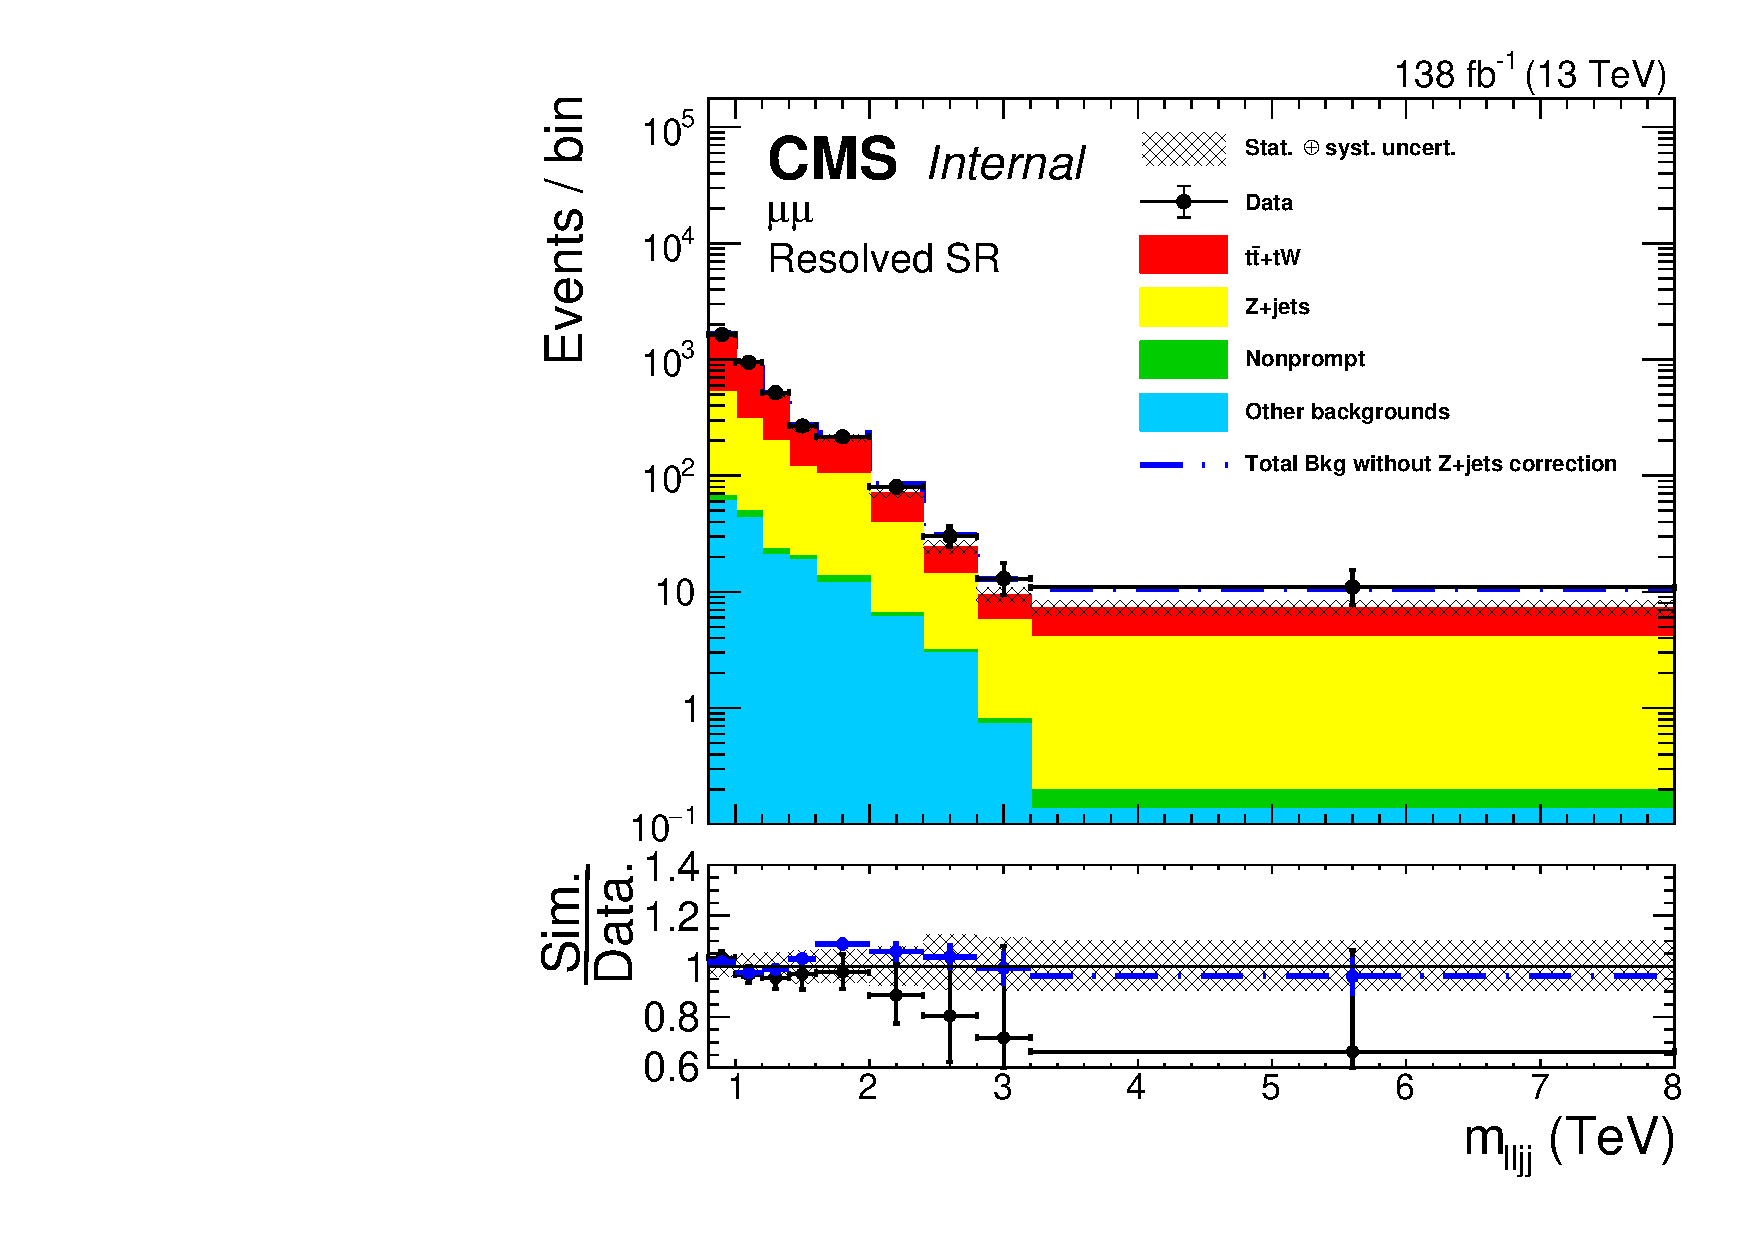
\includegraphics[width=\textwidth]{../figures/plots/mlljj-sr-mumu.pdf}
      \end{column}
      \begin{column}{0.50\textwidth}
          \centering
          \resizebox{0.55\columnwidth}{!}{%
          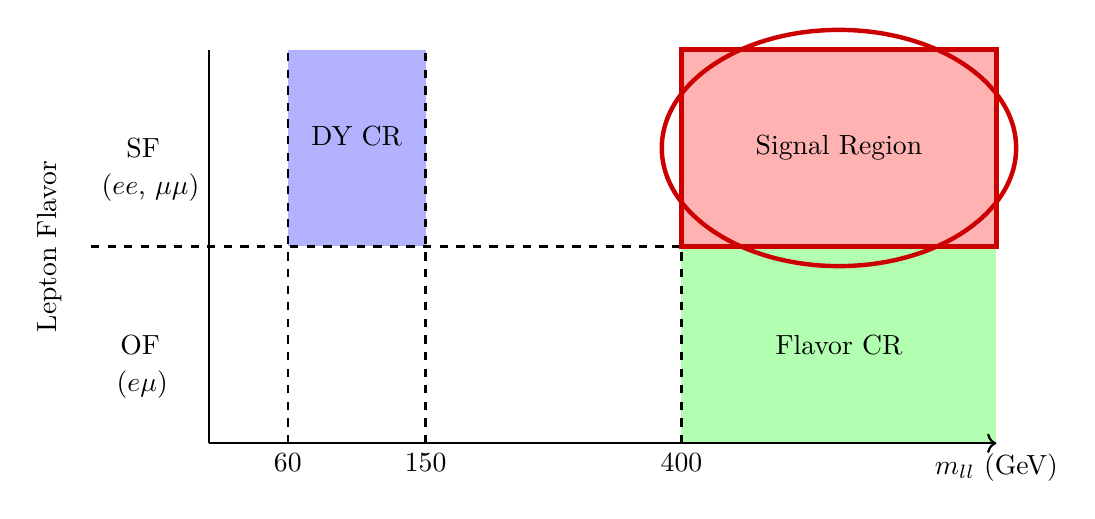
\begin{tikzpicture}[scale=5]
  
    % Define the division points for the vertical regions
    \def\xzero{0.2}   % New left margin division (empty or used for spacing)
    \def\xone{0.55}   % Right boundary of region 1 (DYCR)
    \def\xtwo{1.2}   % Right boundary of region 2 (CR)/left boundary of region 3 (SB)
    \def\xmax{2}      % Overall width of the box

    % -- Fill each grid cell with distinct colors --
    % Column 1: between xzero and xone
    \fill [blue!30!white]    (\xzero,0.5) rectangle (\xone,1);   % Top cell
    \fill [white]    (\xzero,0) rectangle (\xone,0.5);      % Bottom cell

    % Column 2: between xone and xtwo
    \fill [white]   (\xone,0.5) rectangle (\xtwo,1);       % Top cell
    \fill [white]   (\xone,0) rectangle (\xtwo,0.5);         % Bottom cell

    % Column 3: between xtwo and xmax
    \fill [red!30!white]  (\xtwo,0.5) rectangle (\xmax,1);         % Top cell
    \fill [green!30!white]  (\xtwo,0) rectangle (\xmax,0.5);           % Bottom cell
      
    % -- Draw dashed vertical division lines --
    \draw[dashed,thick] (\xzero,0) -- (\xzero,1);  % New left margin boundary
    \draw[dashed,thick] (\xone,0) -- (\xone,1);
    \draw[dashed,thick] (\xtwo,0) -- (\xtwo,1);
    
    % -- Draw a horizontal dashed line (dividing the rows) --
    \draw[dashed,thick] (-0.3,0.5) -- (\xmax,0.5);
    
    % -- Label the y-axis regions (lepton charges) --
    \draw
      (-0.1,0.75) node[anchor=east] {SF}
      (0,0.65) node[anchor=east] {($ee$, $\mu\mu$)}
      (-0.1,0.25) node[anchor=east] {OF}
      (-0.08,0.15) node[anchor=east] {($e\mu$)};
    
    % -- Label the x-axis tick marks (using the original vertical lines) --
    \draw
      (\xzero,0) node[anchor=north] {60}
      (\xone,0) node[anchor=north] {150}
      (\xtwo,0) node[anchor=north] {400};
    
    % -- Axis description on the left --
    \draw
      (-0.35,0.5) node[rotate=90,anchor=south] {Lepton Flavor};
    
    % -- Draw the x-axis as an arrow along the bottom edge --
    \draw[->, thick] (0,0) -- (\xmax,0) node[anchor=north] {$m_{ll}$ (GeV)};
    
    % -- Optionally draw the y-axis line --
    \draw[thick] (0,0) -- (0,1);

    % -- Add internal region labels --
    % Place the label for the DYCR region at the center of the first (red) column:
    \draw ({(\xzero+\xone)/2},0.78) node {DY CR};
    % Place the label for the CR region in the center of the second (blue) column (here using the bottom half for example):
    \draw ({\xtwo+(\xmax-\xtwo)/2},0.25) node[align=center] {Flavor CR};
    % Place the label for the SB region in the center of the third (green) column (using the top half):
    \draw ({\xtwo+(\xmax-\xtwo)/2},0.75) node[align=center] {Signal Region};

      % 1) Outline
    \draw[ultra thick, red!80!black]
      (\xtwo,0.5) rectangle (\xmax,1);

    % 2) Or draw a circle
    \draw[ultra thick, red!80!black]
    ({(\xtwo+\xmax)/2},0.75) 
    ellipse [x radius=0.45, y radius=0.30];

\end{tikzpicture}
          }
  
        \vfill
        \boldcol{UMNMaroon}{The lead jet $p_{T}$ has been reweighted in previous studies.}
        
        \begin{block}{Reweighting with the lead jet $p_T$}
          \begin{itemize}
            \item Before the correction, there is good agreement.
            \item The corrections pulls the MC down, out of agreement.
            \item Excess data isn't very peak-like.
          \end{itemize}
        \end{block}
      \end{column}
    \end{columns}
  \end{frame}
  
  \note[itemize]{
    \footnotesize
    \item A previous verision of this analysis did unblind, except they used the leading jet $p_T$ spectrum to 
     reweight on. And here are the results for the signal region. 
    \item So the way to read this is that the Drell-Yan is already reweighted to the leading jet $p_T$, and 
    this blue line shows what the previous background was before applying that correction.
    \item And so we see that there is initally good agreement between our uncorrected backgrounds and data, 
      and then once we apply the leading jet pt reweighting factors, we pull down our background out of agreement 
      with data.
    \item Naively, you could interpret this by saying that the leading jet pt correction worked, and this excess data that 
    we now observe in our signal region is just signal. These are right-handed W's. And that would be nice, but it is not 
    likely, since for signal we would expect a much more narrow peak, whereas the discrepancy we observe in our signal region 
    here is a much more continuous slope spanning multiple TeV, which suggests that we have a modelling problem instead of 
    actual signal. 
    \item Hence this is why we are shifting to other variables in the future.
  }

  \begin{frame}{Seesaw Mechanism}
    \begin{figure}
      \centering
      
\includegraphics[width=0.70\textwidth]{seesaw-mechanism.png}
      \caption{In LRSM models the lightness of SM neutrinos is explained
      via the seesaw mechanism. Artwork by Sandbox Studio, Chicago with Ana Kova.}
    \end{figure}
  \end{frame}
  
  \note[itemize]{
  \item There are some neutrino people in the audience today, so I'll just mention one more reason
    why left-right symmetric models are appealing is that they provide an explanation for the tiny,
    but non-zero, mass of the left-handed standard model neutrino.
  \item It does this with something called the see-saw mechanism, which describes the lightness of the 
    left-handed standard model neutrino as the result of a suppression effect from a massive right-handed
    neutrino.
  \item And so if the parity restoration doesn't do it for you, maybe neutrino masses are a 
    better motivator.
  }

  \begin{frame}{LHC}
    \begin{figure}
      \centering
      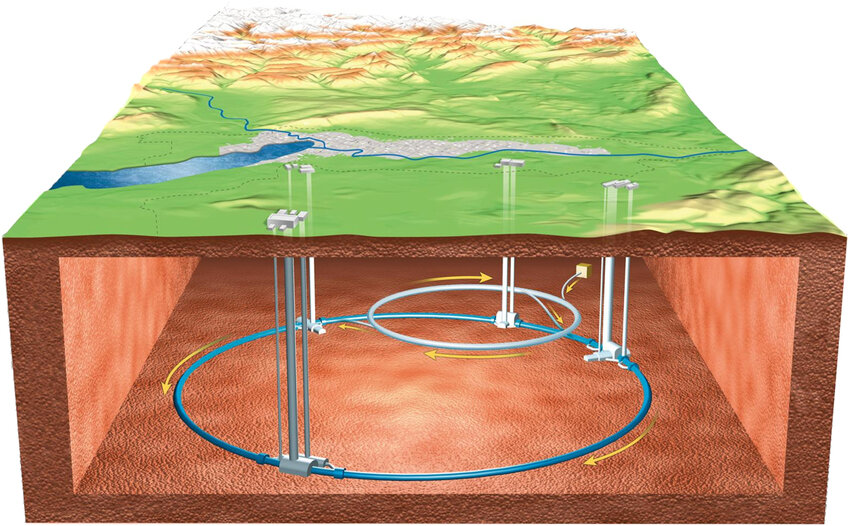
\includegraphics[width=0.7\textwidth]{../figures/experiment/lhc-schematic.png}
      \caption{Schematic showing the overall layout of the LHC. Image credit -- CERN.}
    \end{figure}
  \end{frame}
  
  \note[itemize]{
    \item We search for the right-handed W at the Large Hadron Collider.
    \item The Large Hadron Collider is the worlds most powerful particle accelerator.
    \item  It is located 100 meters underground at CERN, and it accelerates
      beams of protons in opposite directions around a 27km ring. 
    \item The accelerator sits 100 meters underground at CERN in Geneva, and consists 
      of a 27 kilometer ring of superconducting magnets. 
    \item These beams are brought to collide at 4 interaction points with a center of mass 
      energy of 13.6 TeV. 
    \item The particular detector we are using to look for the right-handed W is the CMS 
      (Compact Muon Solenoid) Detector.
  }

\end{backup}

\end{document} 
